%%%%%%%%%%%%%%%%%%%%%%%%%%%%%%%%%%%%%%%%%
% University Assignment Title Page 
% LaTeX Template
% Version 1.0 (27/12/12)
%
% This template has been downloaded from:
% http://www.LaTeXTemplates.com
%
% Original author:
% WikiBooks (http://en.wikibooks.org/wiki/LaTeX/Title_Creation)
%
% License:
% CC BY-NC-SA 3.0 (http://creativecommons.org/licenses/by-nc-sa/3.0/)
% 
% Instructions for using this template:
% This title page is capable of being compiled as is. This is not useful for 
% including it in another document. To do this, you have two options: 
%
% 1) Copy/paste everything between \begin{document} and \end{document} 
% starting at \begin{titlepage} and paste this into another LaTeX file where you 
% want your title page.
% OR
% 2) Remove everything outside the \begin{titlepage} and \end{titlepage} and 
% move this file to the same directory as the LaTeX file you wish to add it to. 
% Then add %%%%%%%%%%%%%%%%%%%%%%%%%%%%%%%%%%%%%%%%%
% University Assignment Title Page 
% LaTeX Template
% Version 1.0 (27/12/12)
%
% This template has been downloaded from:
% http://www.LaTeXTemplates.com
%
% Original author:
% WikiBooks (http://en.wikibooks.org/wiki/LaTeX/Title_Creation)
%
% License:
% CC BY-NC-SA 3.0 (http://creativecommons.org/licenses/by-nc-sa/3.0/)
% 
% Instructions for using this template:
% This title page is capable of being compiled as is. This is not useful for 
% including it in another document. To do this, you have two options: 
%
% 1) Copy/paste everything between \begin{document} and \end{document} 
% starting at \begin{titlepage} and paste this into another LaTeX file where you 
% want your title page.
% OR
% 2) Remove everything outside the \begin{titlepage} and \end{titlepage} and 
% move this file to the same directory as the LaTeX file you wish to add it to. 
% Then add %%%%%%%%%%%%%%%%%%%%%%%%%%%%%%%%%%%%%%%%%
% University Assignment Title Page 
% LaTeX Template
% Version 1.0 (27/12/12)
%
% This template has been downloaded from:
% http://www.LaTeXTemplates.com
%
% Original author:
% WikiBooks (http://en.wikibooks.org/wiki/LaTeX/Title_Creation)
%
% License:
% CC BY-NC-SA 3.0 (http://creativecommons.org/licenses/by-nc-sa/3.0/)
% 
% Instructions for using this template:
% This title page is capable of being compiled as is. This is not useful for 
% including it in another document. To do this, you have two options: 
%
% 1) Copy/paste everything between \begin{document} and \end{document} 
% starting at \begin{titlepage} and paste this into another LaTeX file where you 
% want your title page.
% OR
% 2) Remove everything outside the \begin{titlepage} and \end{titlepage} and 
% move this file to the same directory as the LaTeX file you wish to add it to. 
% Then add %%%%%%%%%%%%%%%%%%%%%%%%%%%%%%%%%%%%%%%%%
% University Assignment Title Page 
% LaTeX Template
% Version 1.0 (27/12/12)
%
% This template has been downloaded from:
% http://www.LaTeXTemplates.com
%
% Original author:
% WikiBooks (http://en.wikibooks.org/wiki/LaTeX/Title_Creation)
%
% License:
% CC BY-NC-SA 3.0 (http://creativecommons.org/licenses/by-nc-sa/3.0/)
% 
% Instructions for using this template:
% This title page is capable of being compiled as is. This is not useful for 
% including it in another document. To do this, you have two options: 
%
% 1) Copy/paste everything between \begin{document} and \end{document} 
% starting at \begin{titlepage} and paste this into another LaTeX file where you 
% want your title page.
% OR
% 2) Remove everything outside the \begin{titlepage} and \end{titlepage} and 
% move this file to the same directory as the LaTeX file you wish to add it to. 
% Then add \input{./title_page_1.tex} to your LaTeX file where you want your
% title page.
%
%%%%%%%%%%%%%%%%%%%%%%%%%%%%%%%%%%%%%%%%%
%\title{Title page with logo}
%----------------------------------------------------------------------------------------
%	PACKAGES AND OTHER DOCUMENT CONFIGURATIONS
%----------------------------------------------------------------------------------------

\documentclass[12pt]{report}
\usepackage[english]{babel}
\usepackage[utf8x]{inputenc}
\usepackage{amsmath}
\usepackage{tikz}
\usetikzlibrary{shapes.geometric,arrows}
\tikzstyle{startstop} = [rectangle, rounded corners, minimum width=3cm, minimum height=1cm,text centered, draw=black, fill=red!30]
\tikzstyle{io} = [trapezium, trapezium left angle=70, trapezium right angle=110, minimum width=3cm, minimum height=1cm, text centered, draw=black, fill=blue!30]
\usepackage{graphicx}
\tikzstyle{process} = [rectangle, minimum width=3cm, minimum height=1cm, text centered, draw=black, fill=orange!30]
\tikzstyle{decision} = [diamond, minimum width=3cm, minimum height=1cm, text centered, draw=black, fill=green!30]
\tikzstyle{arrow} = [thick,->,>=stealth]
\usepackage[colorinlistoftodos]{todonotes}
\usepackage{float}
\usepackage{hyperref}
\usepackage{subcaption}
\begin{document}

\begin{titlepage}

\newcommand{\HRule}{\rule{\linewidth}{0.5mm}} % Defines a new command for the horizontal lines, change thickness here

\center % Center everything on the page
 
%----------------------------------------------------------------------------------------
%	HEADING SECTIONS
%----------------------------------------------------------------------------------------
\textsc{\Large AE 417}\\[0.5cm] % Major heading such as course name
\textsc{\large Aircraft Design Lab}\\[0.5cm] % Minor heading such as course title

%----------------------------------------------------------------------------------------
%	TITLE SECTION
%----------------------------------------------------------------------------------------

\HRule \\[0.4cm]
{ \huge \bfseries Aerial Fire Fighter}\\[0.4cm] % Title of your document
\HRule \\[1.5cm]
 
%----------------------------------------------------------------------------------------
%	AUTHOR SECTION
%----------------------------------------------------------------------------------------

\begin{minipage}{0.4\textwidth}
\begin{flushleft} \large
\emph{Designed by:}\\
Mrinalgouda Patil\\
Rushi Lotti\\ % Your name
Shubham Shinde\\
Veda Krishna Vyas\\
Vikas Kurapati\\
Yashasree Vanam\\
\end{flushleft}
\end{minipage}
~
\begin{minipage}{0.4\textwidth}
\begin{flushright} \large
\emph{Under the guidance of:} \\
Dr. Gopal Shevare\\
Dr. Avijit Chatterjee \\
Dr. Arya Hemendra\\
Dr. Ashok Joshi\\
\end{flushright}
\end{minipage}\\[2cm]

% If you don't want a supervisor, uncomment the two lines below and remove the section above
%\Large \emph{Author:}\\
%John \textsc{Smith}\\[3cm] % Your name

%----------------------------------------------------------------------------------------
%	DATE SECTION
%----------------------------------------------------------------------------------------

%{\large \today}\\[2cm] % Date, change the \today to a set date if you want to be precise

%----------------------------------------------------------------------------------------
%	LOGO SECTION
%----------------------------------------------------------------------------------------

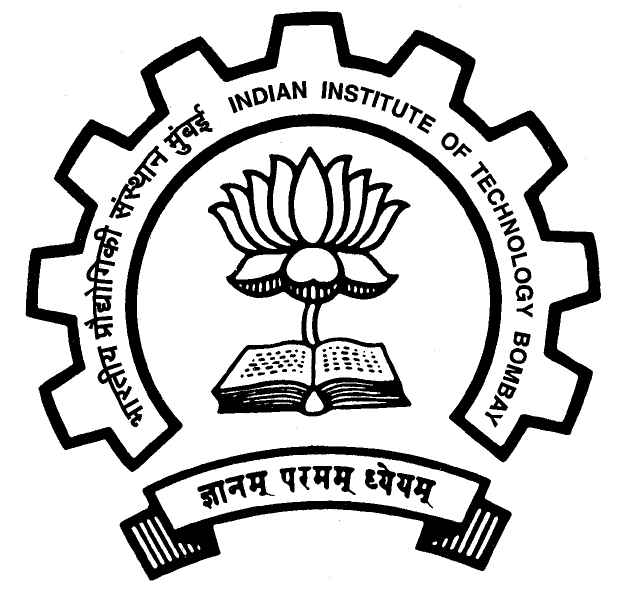
\includegraphics[scale = 0.20]{iitblogo.png} % Include a department/university logo - this will require the graphicx package
 
%----------------------------------------------------------------------------------------

\vfill % Fill the rest of the page with whitespace

\end{titlepage}
\tableofcontents
\newpage
\listoffigures
\newpage
\listoftables

\begin{abstract}
This report deals with the conceptual design of an Unmanned Aerial Vehicle designed to extinguish fires in an urban environment. The problem dictates the travel time and constrains the overall size. A flying wing configuration was chosen from two possible configurations. The ability of vertical take-off and landing were envisaged for the aircraft. Three iterations were performed on the model, each iteration with different design variables. In each iteration, performance calculations and aerodynamic, structural and stability analysis were performed. In performance, mass of fuel consumed was calculated. In aerodynamic analysis, the variations of various aerodynamic coefficients were studied. In structures, we looked into stress and strain distributions across the aircraft. In stability analysis, stability of various modes of vibrations of aircraft was studied. Based on these studies, modifications were made for subsequent iterations.
\end{abstract}

\chapter{Introduction}
Fire is a very good servant, but, a very bad master. As long as fire is under our control, it serves a lot of useful purposes for us, but, once it goes out of our control, it can create a lot of destruction. However, despite the presence of fire safety measures, the occurrence of accidents is oftentimes inevitable. \\
It is this combination (of good servant and bad master), which is dangerous.\\
Because of the useful purposes that it serves, people keep sources of fire in/around their houses/workplace. And, these sources could sometimes result in "undesired" fire. Had fire been something, which serves no useful purpose – the number of incidents of fire would have been very less – as people wont keep sources of fire around them.\\
Thus, the occurrence of fire-related accidents is oftentimes inevitable - inspite of all the safety precautions.\\
So to curb or mitigate the harm casued by fire accidents we have fire extinguishers placed in the houses or fire engines which come to the site of hazard to rescue the people or the objects. However, take the case of a situation where the site of hazard is on the 20th floor of a tall building. In such cases, conventional fire engines will not be of much use as t o reach such height is sometimes difficult. Also, take the case of a situation where nobody is in the house, when the fire accident is broke. Now in such scenarios, the fire extinguisher will be of no use as nobody will be there to use it. So to reduce the destruction caused by the fire hazards, we are designing the flying fire engine which can reach the fire hazard site quickly and mitigate the destructin caused by fire.\\
\chapter{Mission Statement}
\section{Mission Statement}
To design an unmanned flying automobile (fire-engine) which can:
\begin{enumerate}
\item Travel a distance of 18km in a city (inhabitant area)
\item Reach the destination within a time of 10 minutes
\item Carry a payload of 10kg
\item Hover at the destination for 2-3 minutes
\item Can sustain temperatures of around $400^\circ$C (Class A fires)
\end{enumerate}
The numbers mentioned in the Mission Statement are not mere lucky numbers, they have been chosen based on the data available about fire accidents in the city of Mumbai. In Mumbai, there are about 35 fire stations. The average distance between the hazard place and the nearest fire station is around 18km as per the data available in the net. According to the data, the average time taken by the fire engine to reach the hazard site is around 15-20 minutes. So on considering the above numbers associated with the fire stations, we have chosen the average to be traveled by our design has to be around 18km and the time it takes to reach the destination has to be faster than the one mentioned above. So the time it takes to reach has is decided to be 10 minutes.\\
Our flying fire-engine is suited for extinguishing fires of Class A whose temperatures reach a maximum of 400 centigrade. The payload chosen 10kg is based on the fact that this much amount of fire extinguisher is sufficient for extinguishing fire within 1 minute. The payload choosen in our design is compressed carbon-di-oxide. We are assuming the existence of the mechanism by which the fire is extinguished after reaching the destination.
The whole design model is covered using a fire-proof material called calcium silicate, so as to protect the design body from fire.
\section{Customer}
As the mission statement includes numbers which are based on the data studied form the city of Mumbai, the Mumbai Fire Department is the likely customer to the design.
\section{Critical Knowledge}
Ability to hover in hot gases and air with soot is the critical technology. We can see that as the flying body is in the vicinity of the fire, the temperature around will be higher as a result the pressure around (ambient pressure goes up). Now producing the same amount of thrust required to hover at such conditions will be critical. This is because the thrust produced by nozzle is dependent on the ambient temperature. As the ambient pressure increases (room filled with dense gas, smoke), the thrust produced decreases, hence maintain the required amount of thrust is the critical knowledge in this case.
\chapter{Conceptual Design}
Based on mission requirements we decided to go with VTOL as this mechanism helps us perform hover at the hazard site. Since the aircraft operates in urban environment we figured the aircraft might have to move between two buildings. So we constrained our size in any direction to be a maximum of 6 metres which is the width of minimum width of roads in urban area.
\section{Design 1}
This is a fixed wing aircraft that uses jet-engine for propelling and Vertical Take-off and Landing (VTOL). The jet-engine is fixed in position and is connected with a duct which is held horizontal during forward motion and held vertical during hovering, VTOL. The payload is held at the center of gravity of the design. The number of engines used here are 2 fixed to each wing similar to the conventional aircraft.
\begin{figure}[H]
\centering
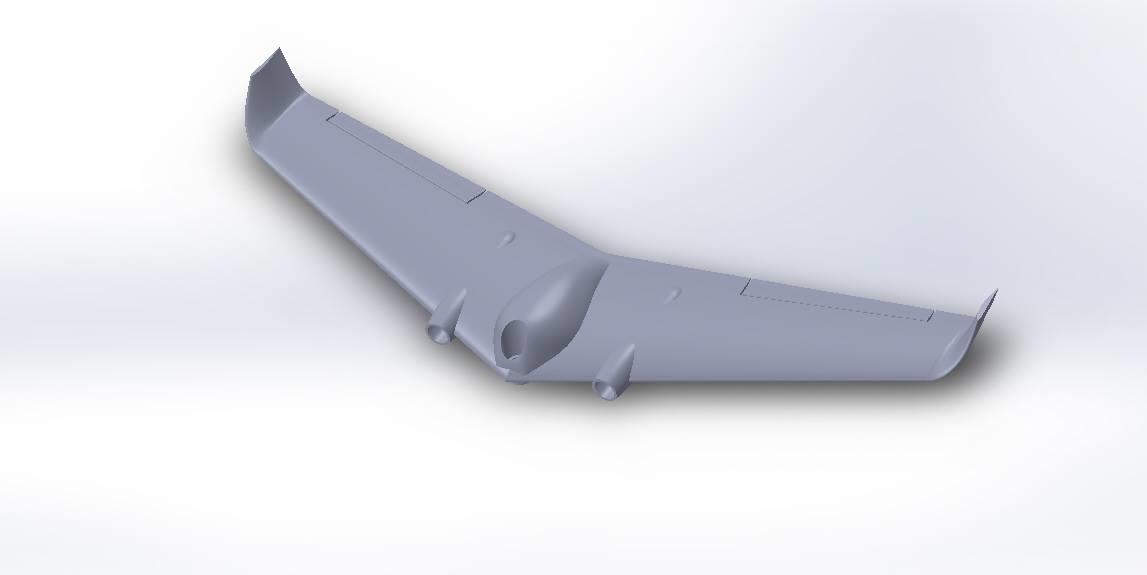
\includegraphics[scale = 0.15]{iter1.png}
\caption{Top and isometric views of the model of Design 1 created using VSP}
\label{Fig3.1}
\end{figure}

\section{Design 2}
This is a rotor-craft consisting of three rotors.  Two small rotors are attached to movable shafts which makes the design maneuverable satisfying one of the mission statement requirements. Using rotors will overcome the problem of hovering at high temperatures as the decrease in density due to increase in density can be compensated by increasing the velocity. The third big rotor serves for lift and thrust. The payload is held at the center of gravity of the rotor-craft.
\begin{figure}[H]
\centering
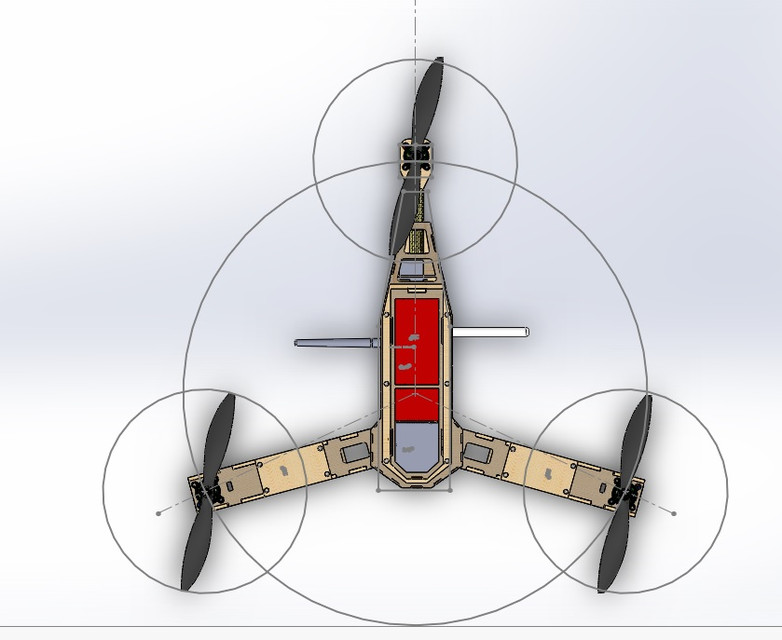
\includegraphics[scale = 0.5]{fig3.jpg}
\caption{Top view of the model of Design 2 using CAD (not scaled)}
\label{Fig3.3}
\end{figure}
\section{Comparison}
The rotor-craft design has an issue of down-wash which will add more oxygen to the fire and increase the fire while this issue will not prevail with the design 1 as the exhaust gases of nozzles barely have oxygen as the exhaust gases are already burnt where they use up the oxygen and hence don’t add up oxygen to the combustion occurring in the fire. Also considering the fact that it is not easy to produce high thrust using rotors as large size rotors are needed.\\ 
After qualitative comparison of two models, we decided to go ahead with the design 1 as the main aim is to curb fire and hence not to enhance the combustion in the fire.
\chapter{Subsystems}
The key physical components, or subsystems, that define the aircraft are the fuselage,
the wings, the horizontal tail, the vertical tail, and the propulsion system. Our design is based
on the flying wing. The flying wing consists of wing with the control surfaces which act as
horizontal stabilizer and the winglets are attached with rudder. Also, a small bulge which is
the fuselage is present in the middle of the wing. This can be seen from Fig1. which shows
the CAD model of the design.
\section{Subsystems to be Designed}
The subsystems which are designed by the team include the following
\begin{enumerate}
\item Wing 
\item Control Surfaces
\item Nacelles for Engine
\item Fuselage
\end{enumerate}
\section{Subsystems to be bought}
The subsystems which are bought from the external sources include the following:
\begin{enumerate}
\item Hydraulic systems
\item Electrical systems
\item Engine
\item Payload (chemical)
\item GPS tracking system
\item Retractable Pipe system involved in deploying the payload (chemical)
\end{enumerate}
\chapter{Design Methodology}
\begin{center}
\begin{tikzpicture}[node distance=1.25cm]
\node (start) [io] {Weight Estimation};
%\node (in1) [io, below of=start] {Input};
\node (pro1) [process, below of=start] {Engine Analysis};
\node (dec1) [process, below of=pro1] {Point Performance};
\node (dec2) [process, below of=dec1] {Aerodynamic Analysis};
\node (dec3) [process, below of=dec2] {Structural Analysis};
\node (dec4) [process, below of=dec3] {Stability Analysis};
\node (dec5) [process, below of=dec4] {Trim Analysis};
\node (dec6) [process, below of=dec5] {Objective function};
\node (last) [io, below of=dec6] {Modify};
\node (thrust) [decision, right of=dec3, xshift=5cm] {T,W changes are small?};
\draw [arrow] (start) -- (pro1);
\draw [arrow] (pro1) -- (dec1);
\draw [arrow] (dec1) -- (dec2);
\draw [arrow] (dec2) -- (dec3);
\draw [arrow] (dec3) -- (dec4);
\draw [arrow] (dec4) -- (dec5);
\draw [arrow] (dec5) -- (dec6);
\draw [arrow] (dec6) -- (last);
\draw [arrow] (last) -| (thrust);
\draw [arrow] (thrust) |- node[anchor=west] {no}(start);
\draw [arrow] (thrust) |- node[anchor=west] {yes} (dec1);
\end{tikzpicture}
\end{center}
The above flow chart shows the design methodology for every iteration of design being performed.
The design methodology which we have implemented is as follows:
\begin{enumerate}
\item CAD Model - It should show all the necessary features including where we are positioning
the fuel, payload, engine with dimensions. However, these dimensions can be assumed in the
first iteration. We have used softwares like SOLIDWORKS, VSP, XFLR5.
\item  Point Performance - With the assumed model, we look forward to calculate the fuel
consumed in each leg of the flight profile. Here, we can assume the $C_l$, $C_d$ values.
\item Aerodynamic Analysis (CFD or Analytic) - In this we need to calculate the actual $C_L$, $C_D$
values for our configuration by using CFD or Prandtl Lifting line theory or any methods.
\item  Stress Analysis - This involves the structure analysis assuming the structure to be thin-walled
ones. This include Bending Moment, Shear force calculations.
\item Trim, Stability Analysis - Here we have to make stability analysis based on the trim
condition. This includes the sizing of control surfaces and their deflection.
\item  Now we have to change the design variables such that it meets all the necessary
requirements. For example: change in the position of the engine such that the aileron size is
increased or increasing the span of the wing so as to accommodate the larger fuel calculated in
step 2.
\item Now, again we have to make a CAD model for the new configuration.
\end{enumerate}
\chapter{Flight Profile}
\begin{figure}[H]
\centering
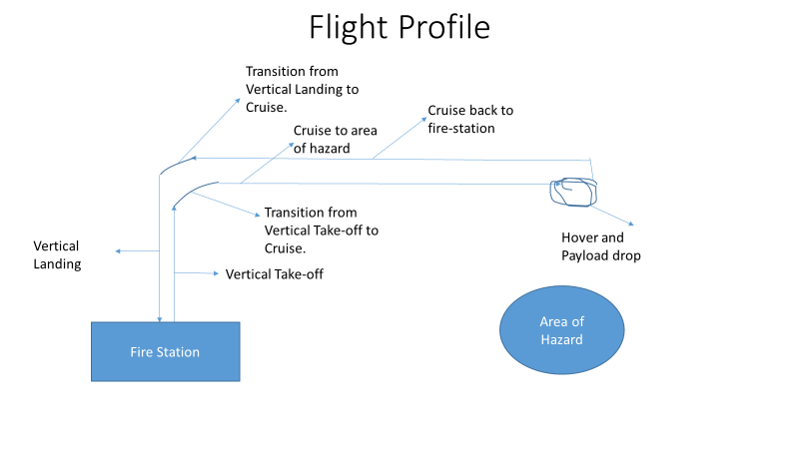
\includegraphics[width = 1.25\textwidth]{fig4.png}
\caption{Flight Profile of the aircraft}
\label{Fig7.1}
\end{figure}

\chapter{Design Variables}
Design variables are the free variables which can be varied by the designer to define a
designed object. The following are the design variables:
\begin{enumerate}
\item Wing Geometry:
\begin{itemize}
\item Airfoil selection
\item Span
\item Chord
\item Placement of fuel
\item Placement of payload
\item Size of Control surfaces
\item Geometry of wing (taper, sweep, twist, dihedral)
\end{itemize}
\item Engine:
\begin{itemize}
\item Type of Engine
\item Placement of Engine
\end{itemize}
\item Structures:
\begin{itemize}
\item Type of material used
\item Internal Geometry of the wing.
\end{itemize}
\end{enumerate}
\chapter{First Iteration}
\section{CAD Model}
\begin{figure}[H]
\centering
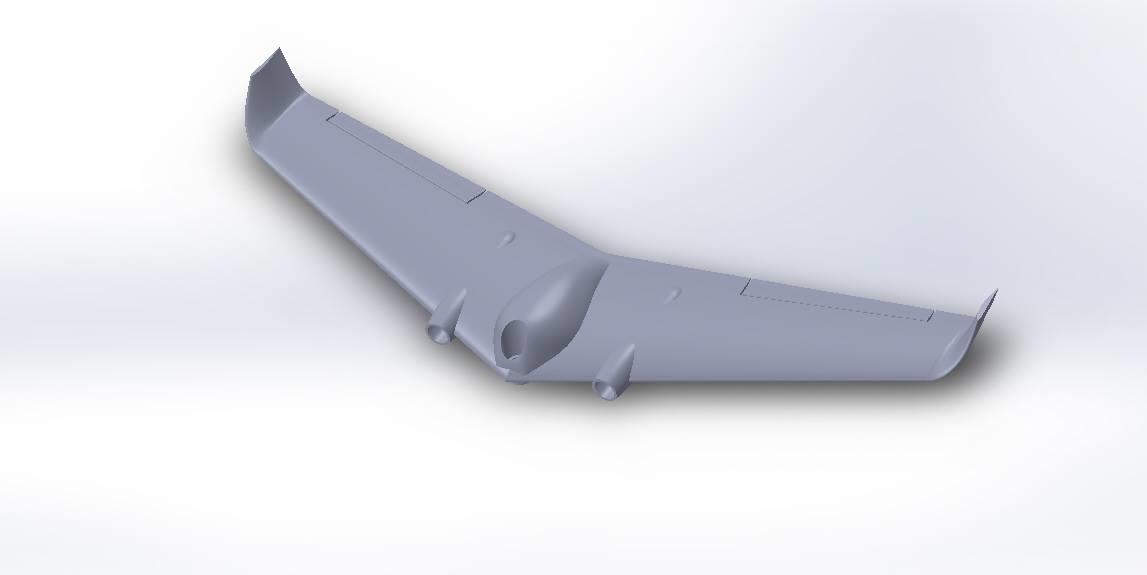
\includegraphics[width = \textwidth]{iter1.png}
\caption{CAD Model of iteration1}
\end{figure}
\begin{figure}[H]
 \centering
 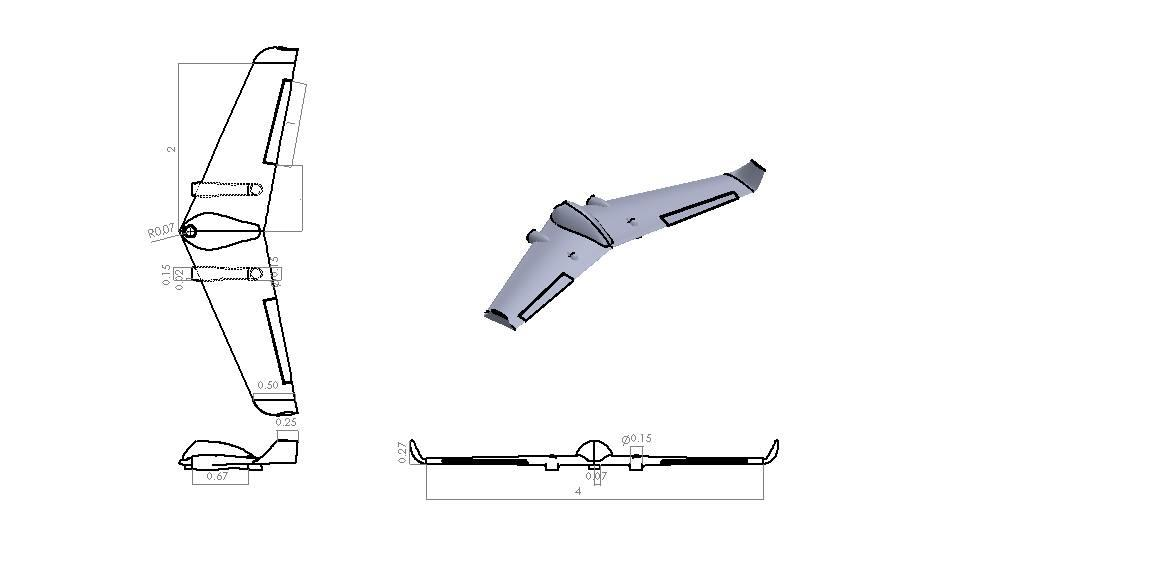
\includegraphics[width = 1.5\textwidth]{iter1-2.png}
 \caption{Dimensions of Iteration1}
\end{figure}

\section{Weight Estimation}
The total estimated weight of the aircraft comes out to be around 210kg. The distribution goes as follows.\\
\begin{table}[H]
\begin{center}
\begin{tabular}{ |c| c| }
\hline
 Wing & 90kg \\ 
 Fuselage & 10kg \\ 
 Control Surfaces & 5 Kg \\ 
 Camera & 5kg \\
 Electronics & 5kg \\
 Ejector System & 5kg \\
 Engine & $3\times7.5$kg \\
 Payload & 10kg \\
 Fuel & 60kg \\
 \hline
 Total & 210kg \\
\hline
\end{tabular}
\end{center}
\caption{Weight Estimation in First Iteration.}
\label{Table1}
\end{table}
Now, we need to calculate thrust required for vertical take-off. \\
We take the acceleration for the take-off to be 0.5$\frac{m}{s^2}$
T = m(g+a) = 210(9.8+0.5) = 2163N \\
%%% Block Diagram%%%
This control block gives the value of $T_1$,$T_2$ based on C.G.
\begin{center}
$M_{cg} = T_1x_{cg1} - 2T_2x_{cg2}$ \\
$T_1x_{cg1} = 2T_2x_{cg2}$ \\
$T_1 + T_2 + T_3 = W$ \\
\end{center}
For vertical take off:
\begin{center}
$d = \frac{1}{2}at^2 \implies 150 = \frac{1}{2}0.5t^2$
t = 25-30s
\end{center}
Hence, assume transition takes place in 20-30 seconds. 
\section{Engine Analysis}
\textbf{Engine Chosen:PBS TJ-40} Given the data from  \url{http://www.pbsvb.com/customer-industries/aerospace/aircraft-engines/tj40-g2-turbojet-engine} \\
$\rho_{air} = 1.225\frac{kg}{m^3}$, $A_C = \frac{\pi d_c^2}{4}$, $\dot{m} = \rho_{air} \times V \times A_C$ \\
$KE_{per mass} = \frac{V^2}{2}$, power = $\dot{m}\times KE_{per mass}$ \\
lift = $\dot{m}V = \rho_{air}\times V\times A_C\times V = \rho_{air}\times V^2 \times \frac{\pi d_c^2}{4}$ \\
$3\dot{m}V_{duct} = m(V_{air} + g) = 210\times 10.3$
\section{Point Performance}
We have 3 main stages in the fight profile namely vertical take-off(VTOF), cruise, hover. We consider transition phase to be negligible, however we carry some extra fuel for that phase. 
\subsection{VTOF}
$m_f = \dot{m_f}\times t = \rho_{fuel}\times A_{duct}\times V \times t$ (t$\sim$60s)
By calculation, $m_f$ comes out to be 4.5 kgs.
\subsection{Cruise}
$R = \frac{V_{cruise}}{C_{cruise}}\times\frac{L}{D}\times0.866 \times ln(\frac{W_{i-1}}{W_i})$ \\
where R is range $V_{cruise}$ is cruise speed, $c_{cruise}$ is the speed of sound in cruise conditions, $\frac{L}{D}$ is lift to drag ratio in cruise conditions and $W_{i-1}, W_i$ are weights before and after the cruise leg respectively.\\
18000 = $\frac{40}{c_{cruise}}\times16\times0.8666\times ln(\frac{W}{W - m_f})$
By calculation, $m_f$ comes out to be 20 kgs.
\subsubsection{Hover}
Hover profile is almost same as VTOF, except we don't have vertical acceleration.\\
So, $V_{duct}$ will be lower.\\
Hence, $m_f = \dot{m_f}\times t$, $\dot{m_f}$ will be less.\\
But time t is of the order of 120-150 s. So, fuel consumed is higher.\\
Hence we take fuel(initial) to be twice the total fuel calculated because of the return path.
By calculation, $m_f$ comes out to be 5.5 kgs.
\section{Aerodynamic Analysis}
For calculating the aerodynamic parameters and stability derivatives, we have used the software called XFLR5.
We have used the Lifting-Line Theory for the calculation and used the fixed-speed analysis. The flow was assumed to be incompressible at a density of 1.225 kg/m3 and viscosity at 1.5 x $10^-5 m^2/s$.
For various aileron positions, we ran simulations and found various graphs that illustrate the relationship between parameters like CL, CD and angle of attack.
The following plots are deduced from the aerodynamic analysis of the aircraft.
\begin{figure}[H]
\begin{subfigure}{0.6\textwidth}
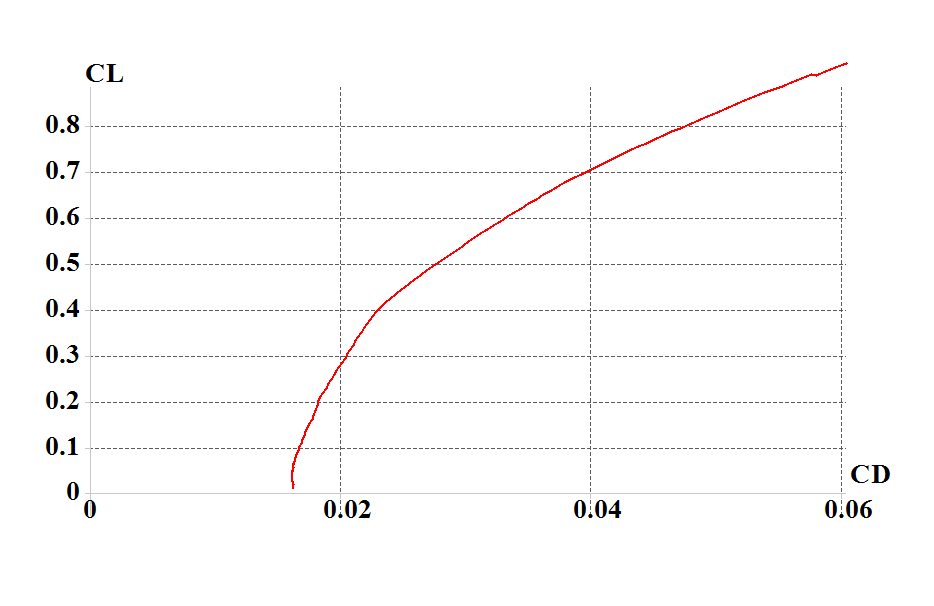
\includegraphics[width = \linewidth]{cl_vs_cd.png}
\caption{$C_l$ vs $C_d$}
\end{subfigure}
\begin{subfigure}{0.6\textwidth}
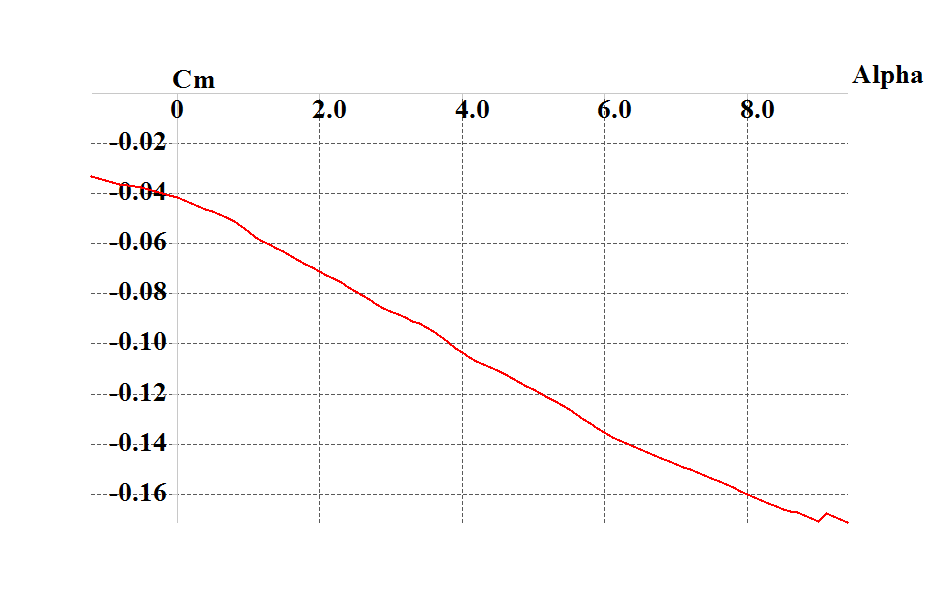
\includegraphics[width = \linewidth]{cm_alpha.png}
\caption{Moment coefficient about Y-axis through C.G. vs $\alpha$}
\end{subfigure}
\medskip
\begin{subfigure}{0.6\textwidth}
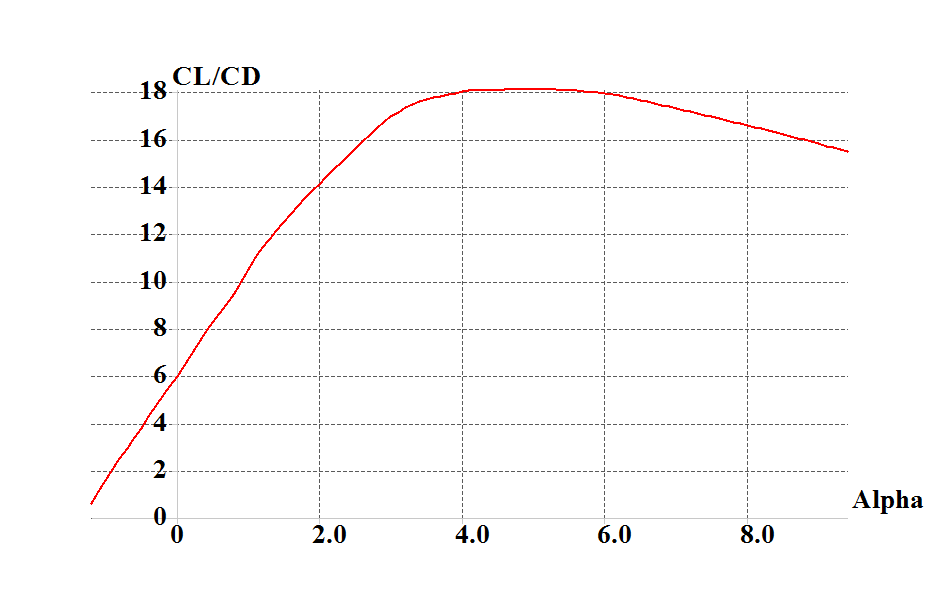
\includegraphics[width = \linewidth]{clcd_vs_alpha.png}
\caption{$\frac{C_l}{C_d}$ vs $\alpha$}
\end{subfigure}
\begin{subfigure}{0.6\textwidth}
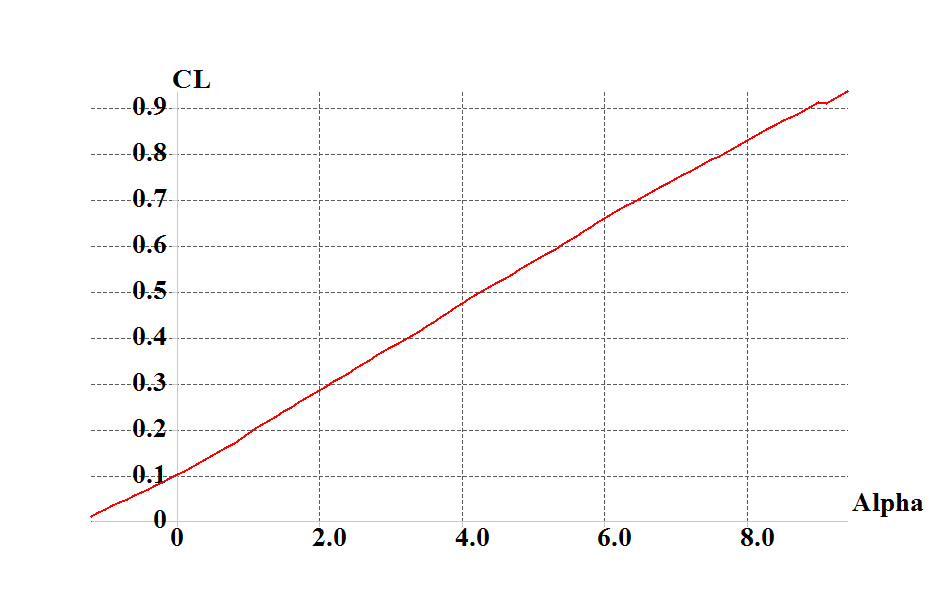
\includegraphics[width = \linewidth]{cl_vs_alpha.png}
\caption{$C_l$ vs $\alpha$}
\end{subfigure}
\caption{Aerodynamic Analysis in First Iteration}
\end{figure}
\section{Trim Analysis}
In order to achieve trim condition, the moment coefficient must be equal to zero. We found that for zero aileron deflection, there was no angle of attack where the moment coefficient was zero. Hence there was no trim condition possible for zero deflection.\\
We ran simulations for different aileron deflections, and we found that the moment coefficient crossed zero for an angle of attack of 6.2 degrees at an aileron deflection of 40 degrees.\\
The slope of moment coefficient and angle of attack was found to be negative. Hence, if a gust causes a decrease in angle of attack, it will result in a positive pitching moment, a tendency to go back to the trim condition. Likewise, a perturbation that elevates angle of attack to a higher value will generate a negative pitching moment, again a tendency to back to the trim. Negative slope, or in other words, negative $c_{m_\alpha}$ is a requirement for longitudinal static stability.\\
After running a stability analysis, the trim condition was reconfirmed at a deflection of 40 degrees. The stability analysis of that state has been provided below.\\

\section{Stability Analysis}
The stability analysis was performed for the trim condition of 40 degrees aileron deflection and 6.2 degrees angle of attack.
The following are the time response plots of the five modes. The modes are decoupled, which enables us to study each mode in isolation, unlike in a real world scenario where the actual response is the sum of all five modes of instability.
It can be inferred that the aircraft was stable in all modes.
\begin{table}[H]
\begin{center}
\begin{tabular}{ |c| c| c| }
\hline
 Mode & Damping & Frequency(Hz) \\ 
 \hline
 Phugoid Mode & 0.050 & 0.026 \\ 
 \hline
 Short Period & 0.234 & 1.601 \\ 
 %Roll subsidence Mode & 1 & 0 \\
 \hline
 Dutch Roll Mode & 0.024 & 0.322 \\
 %Spiral Mode & 1 & 0 \\
 \hline
\end{tabular}
\end{center}
\caption{Damping and Frequencies for various modes.}
\end{table}

\subsection{Roll Mode}
\begin{figure}[H]
\begin{subfigure}{0.48\textwidth}
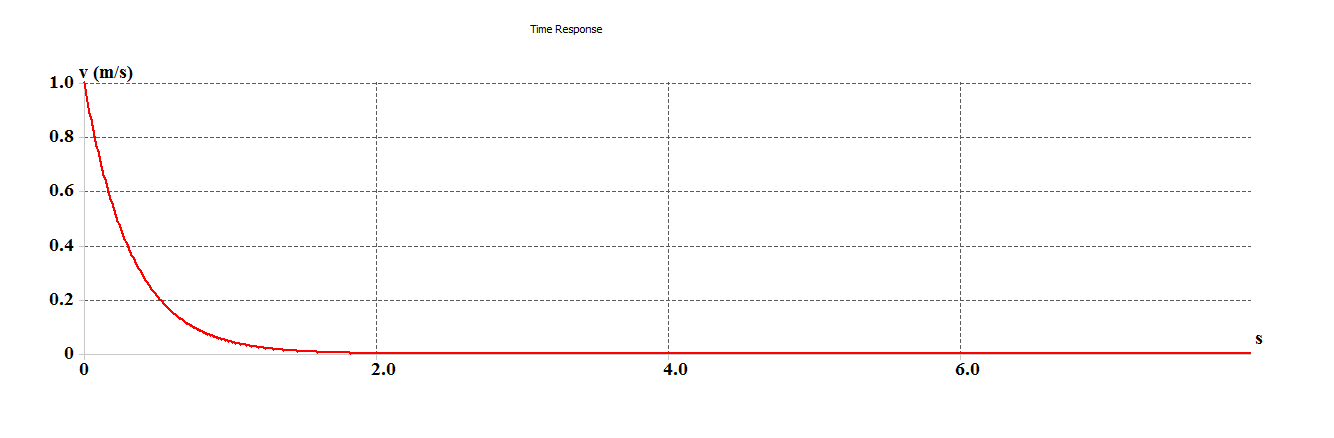
\includegraphics[width = \linewidth]{v.png}
\end{subfigure}
\begin{subfigure}{0.48\textwidth}
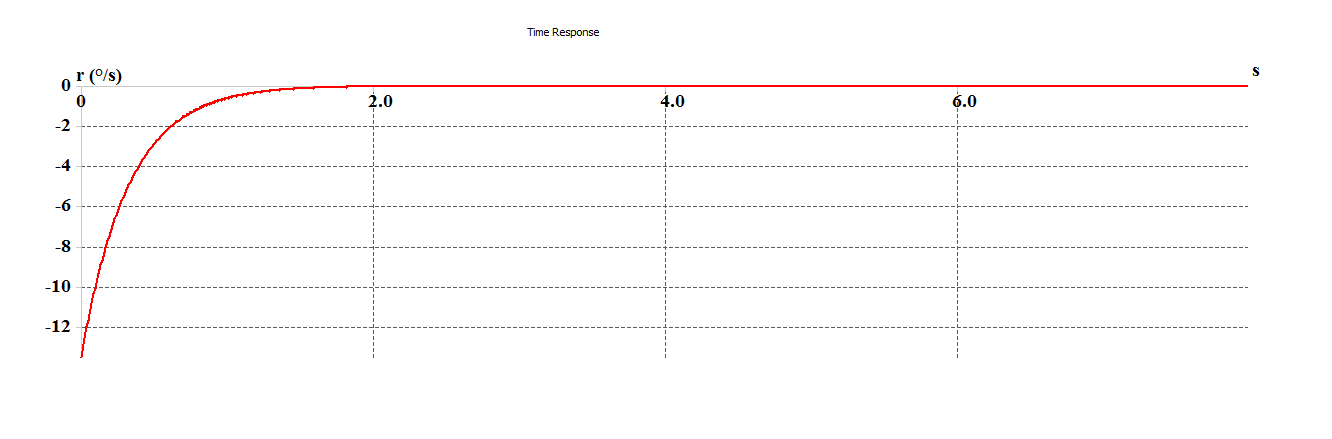
\includegraphics[width = \linewidth]{r.png}
\end{subfigure}
\medskip
\begin{subfigure}{0.48\textwidth}
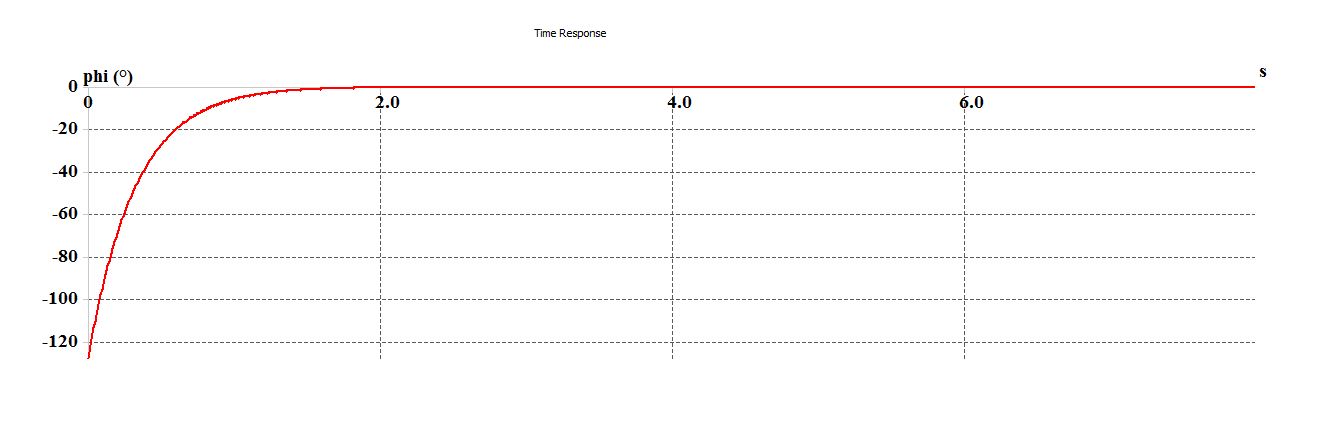
\includegraphics[width = \linewidth]{phi.png}
\end{subfigure}
\begin{subfigure}{0.48\textwidth}
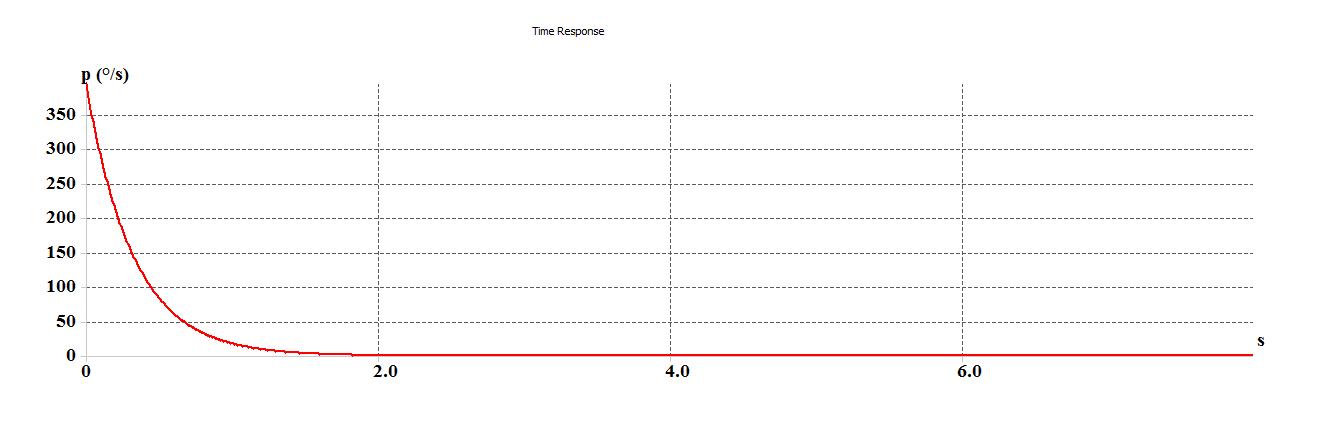
\includegraphics[width = \linewidth]{p.png}
\end{subfigure}
\caption{Roll Mode Analysis in First Iteration}
\end{figure}
\subsection{Phugoid Mode}
\begin{figure}[H]
\begin{subfigure}{0.48\textwidth}
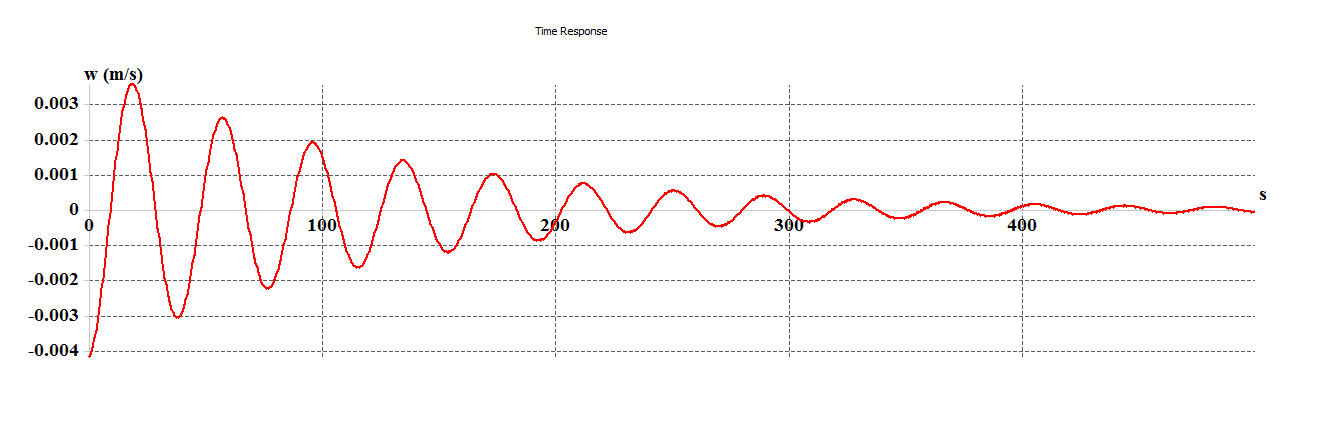
\includegraphics[width = \linewidth]{w.png}
\end{subfigure}
\begin{subfigure}{0.48\textwidth}
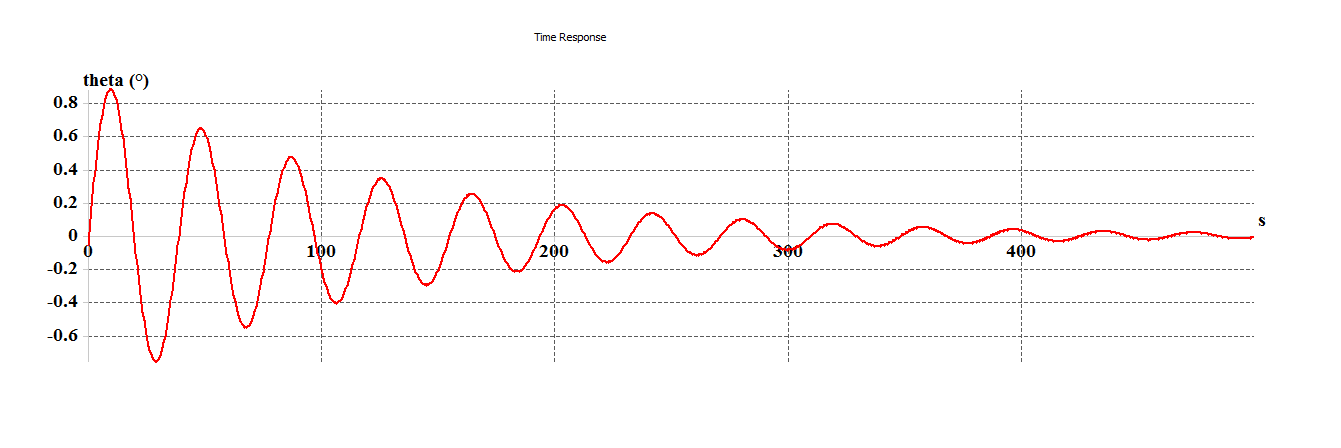
\includegraphics[width = \linewidth]{theta.png}
\end{subfigure}
\medskip
\begin{subfigure}{0.48\textwidth}
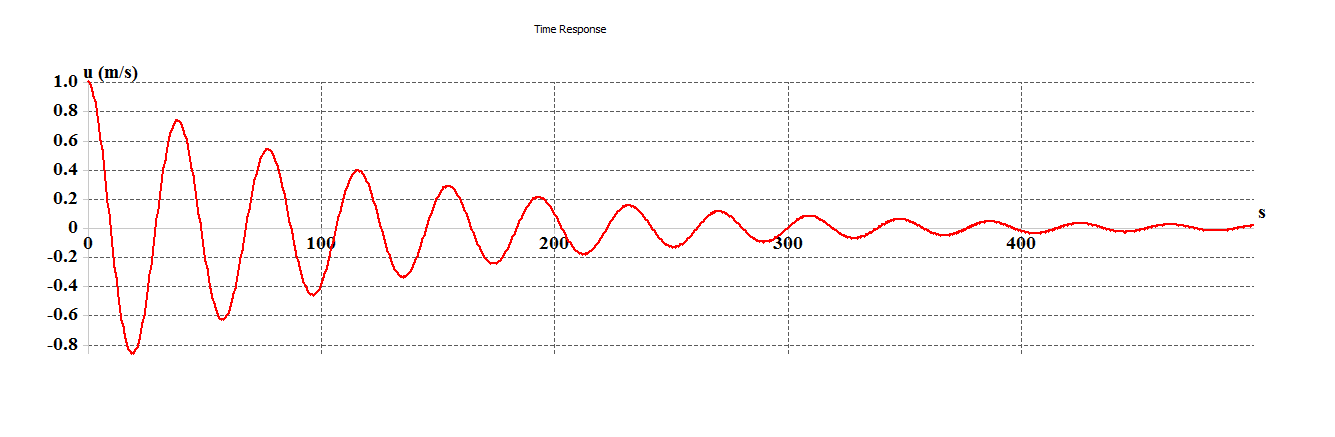
\includegraphics[width = \linewidth]{u.png}
\end{subfigure}
\begin{subfigure}{0.48\textwidth}
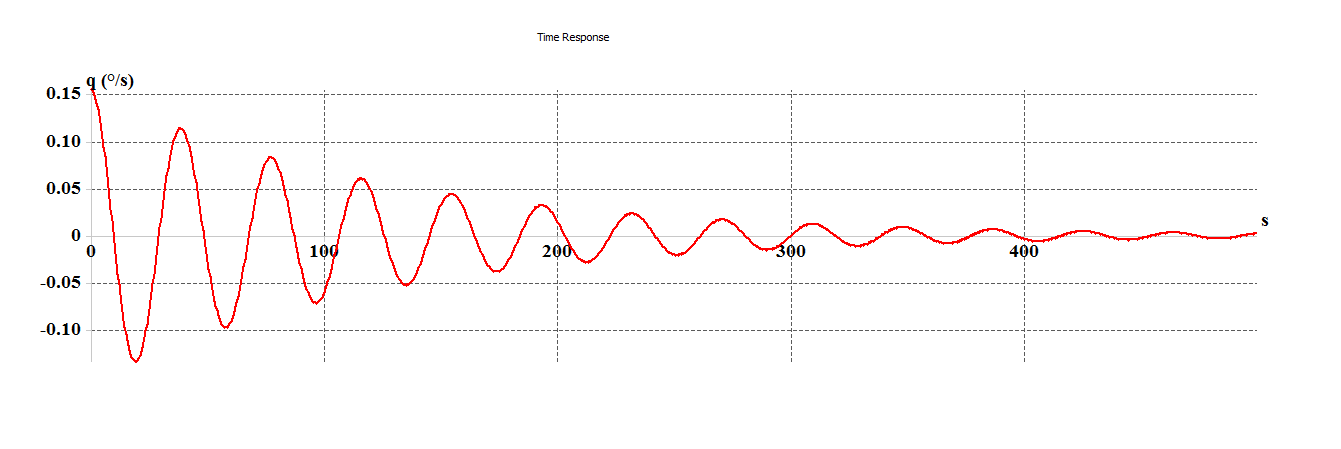
\includegraphics[width = \linewidth]{q.png}
\end{subfigure}
\caption{Phugoid Mode Analysis in First Iteration}
\end{figure}
\subsection{Dutch Roll Mode}
\begin{figure}[H]
\begin{subfigure}{0.48\textwidth}
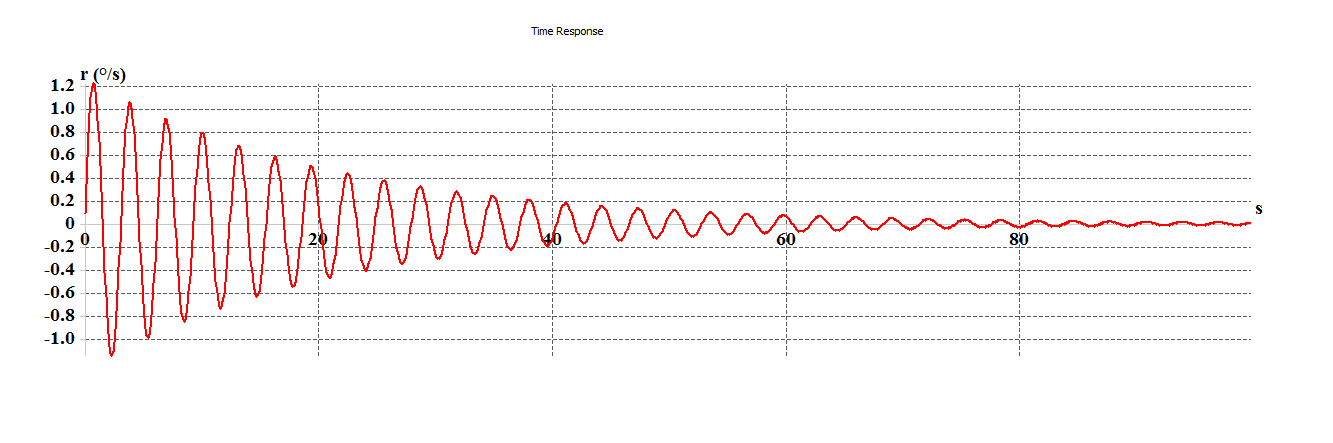
\includegraphics[width = \linewidth]{r__1_.png}
\end{subfigure}
\begin{subfigure}{0.48\textwidth}
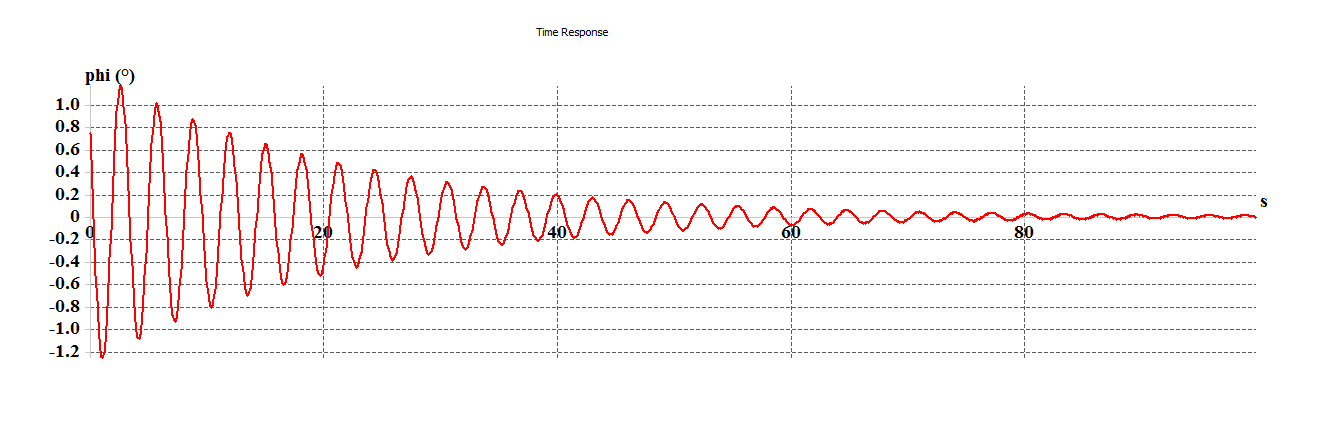
\includegraphics[width = \linewidth]{phi__1_.png}
\end{subfigure}
\medskip
\begin{subfigure}{0.48\textwidth}
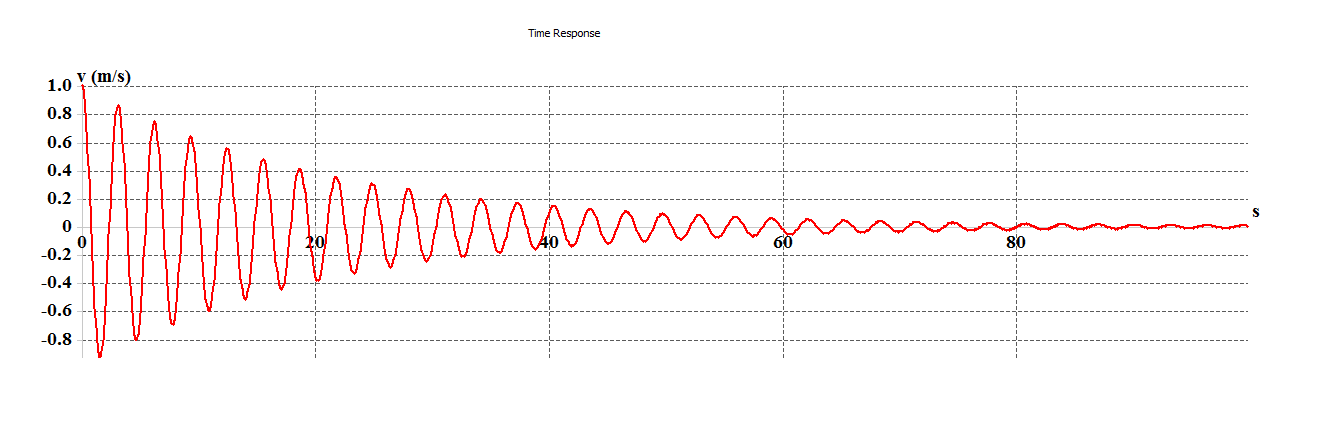
\includegraphics[width = \linewidth]{v__1_.png}
\end{subfigure}
\begin{subfigure}{0.48\textwidth}
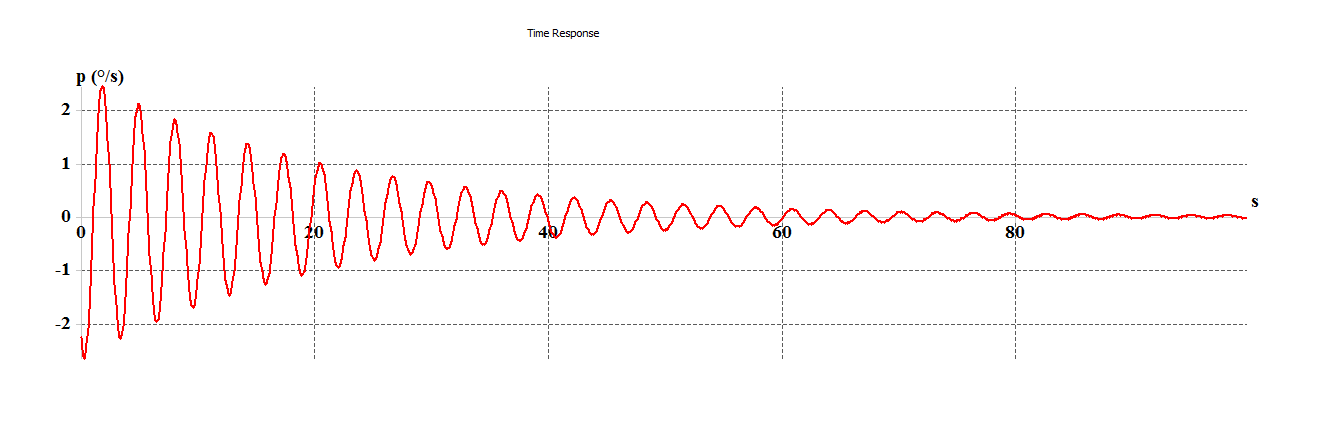
\includegraphics[width = \linewidth]{p__1_.png}
\end{subfigure}
\caption{Dutch Roll Mode Analysis in First Iteration}
\end{figure}
\subsection{Spiral Mode}
\begin{figure}[H]
\begin{subfigure}{0.48\textwidth}
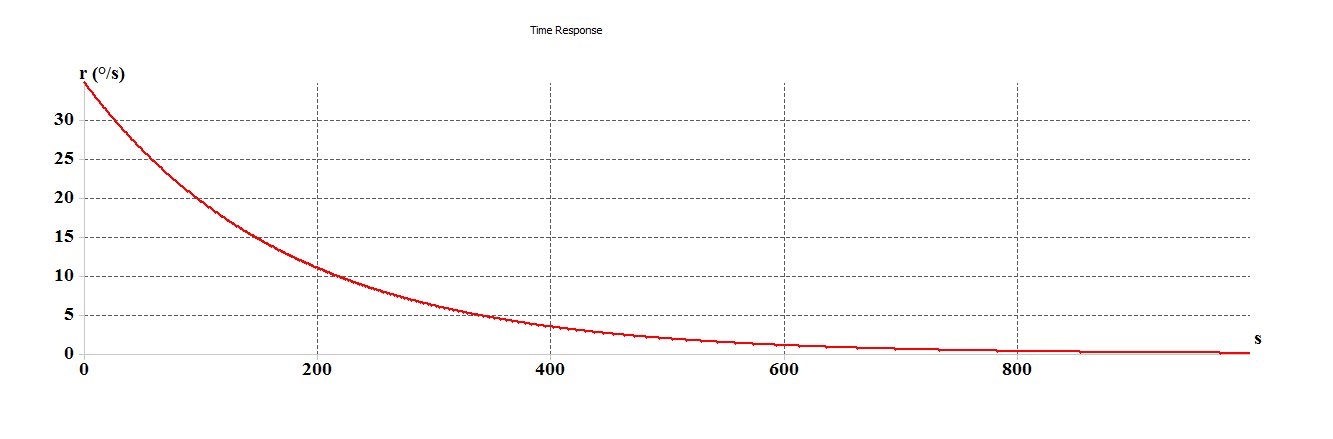
\includegraphics[width = \linewidth]{r__2_.png}
\end{subfigure}
\begin{subfigure}{0.48\textwidth}
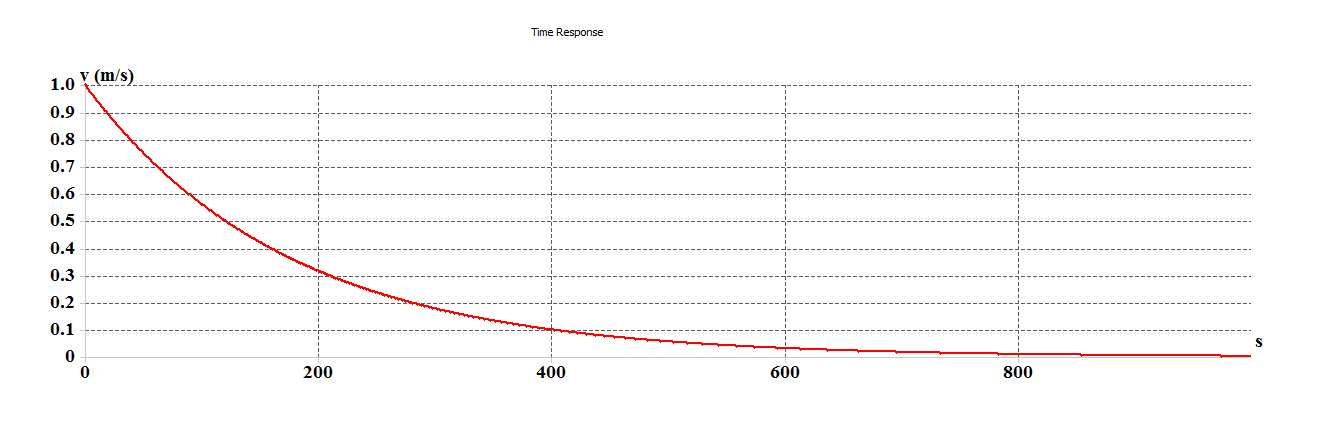
\includegraphics[width = \linewidth]{v__2_.png}
\end{subfigure}
\medskip
\begin{subfigure}{0.48\textwidth}
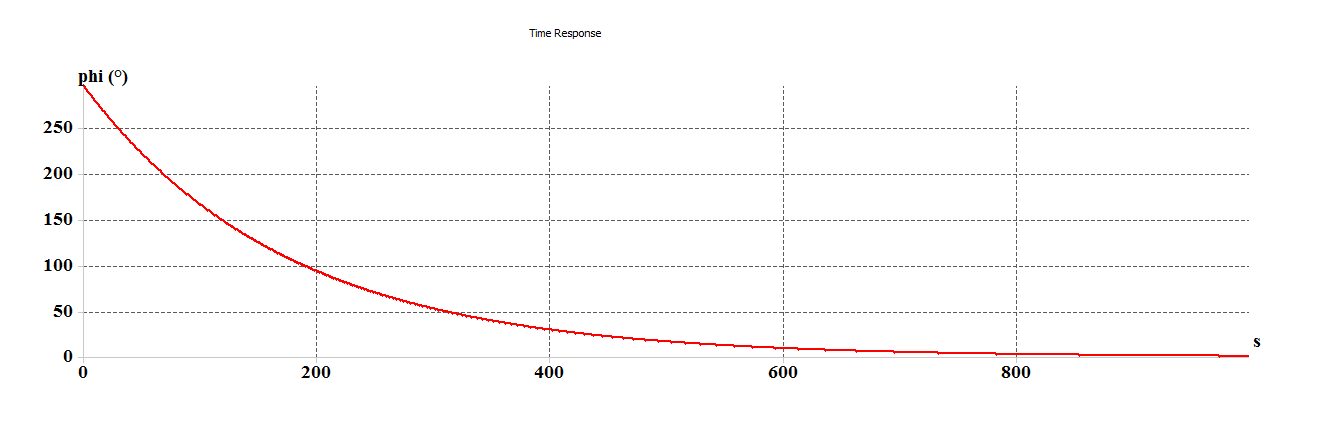
\includegraphics[width = \linewidth]{phi__2_.png}
\end{subfigure}
\begin{subfigure}{0.48\textwidth}
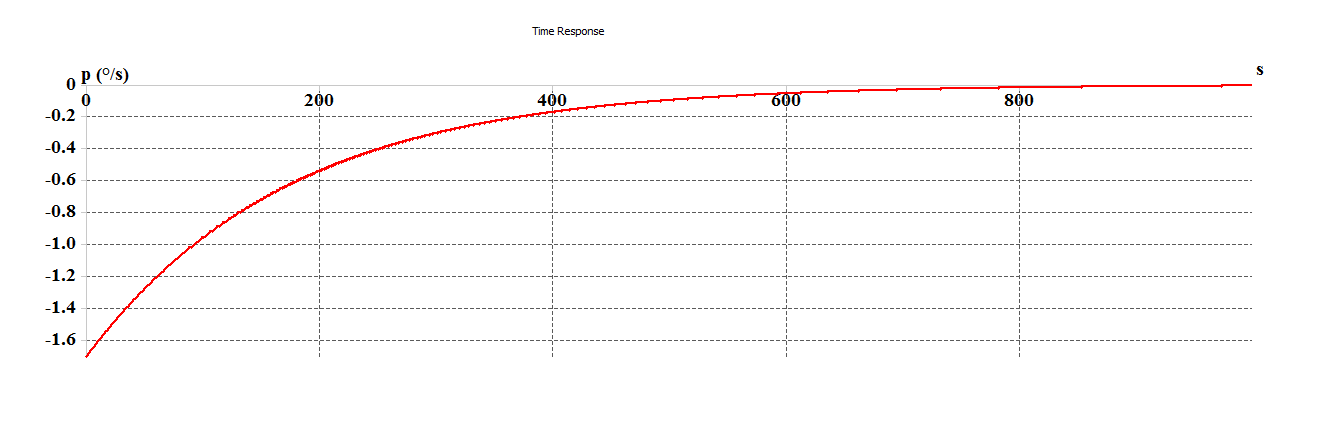
\includegraphics[width = \linewidth]{p__2_.png}
\end{subfigure}
\caption{Spiral Mode Analysis in First Iteration}
\end{figure}
\subsection{Short Period Mode}
\begin{figure}[H]
\begin{subfigure}{0.48\textwidth}
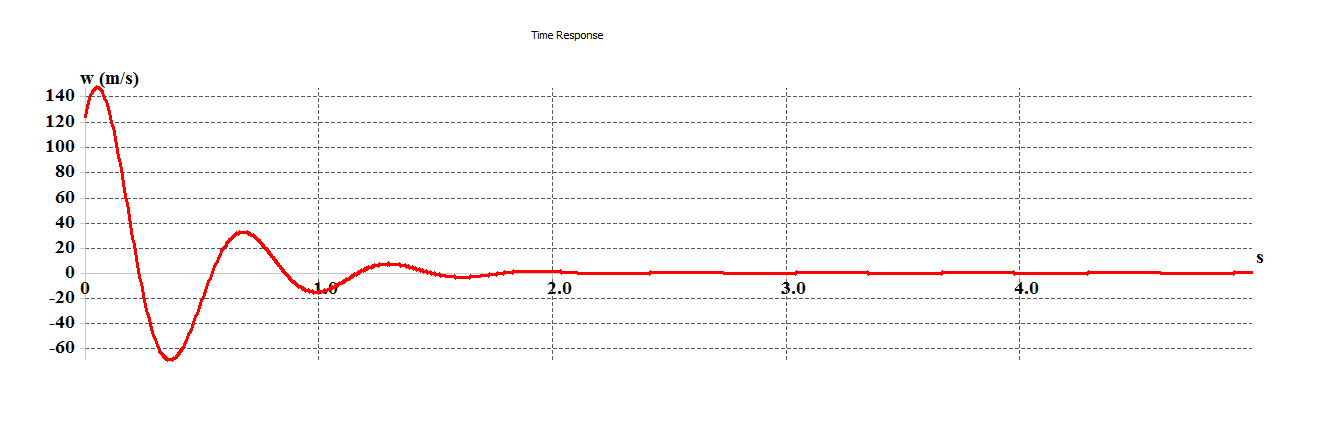
\includegraphics[width = \linewidth]{w__1_.png}
\end{subfigure}
\begin{subfigure}{0.48\textwidth}
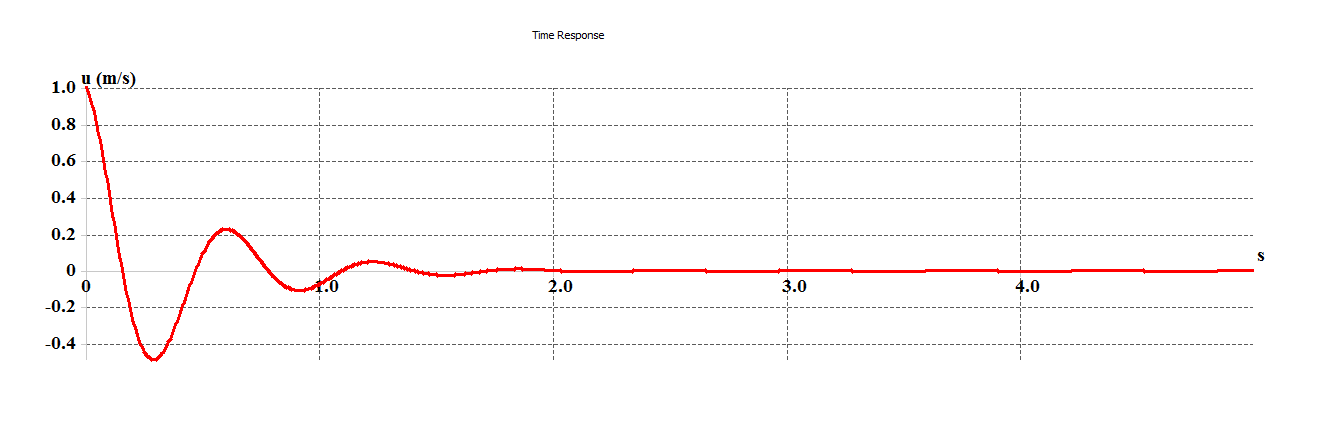
\includegraphics[width = \linewidth]{u__1_.png}
\end{subfigure}
\medskip
\begin{subfigure}{0.48\textwidth}
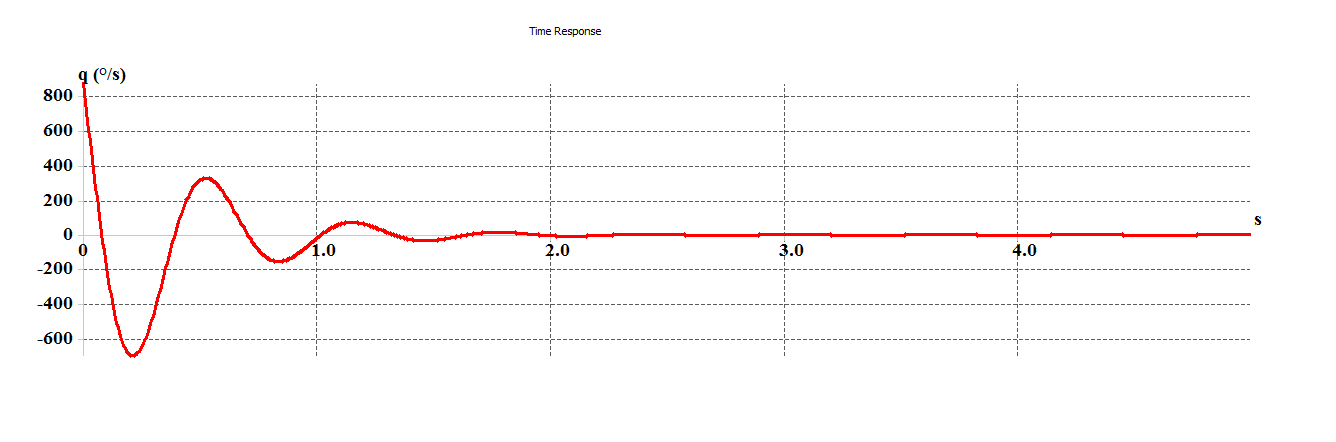
\includegraphics[width = \linewidth]{q__1_.png}
\end{subfigure}
\begin{subfigure}{0.48\textwidth}
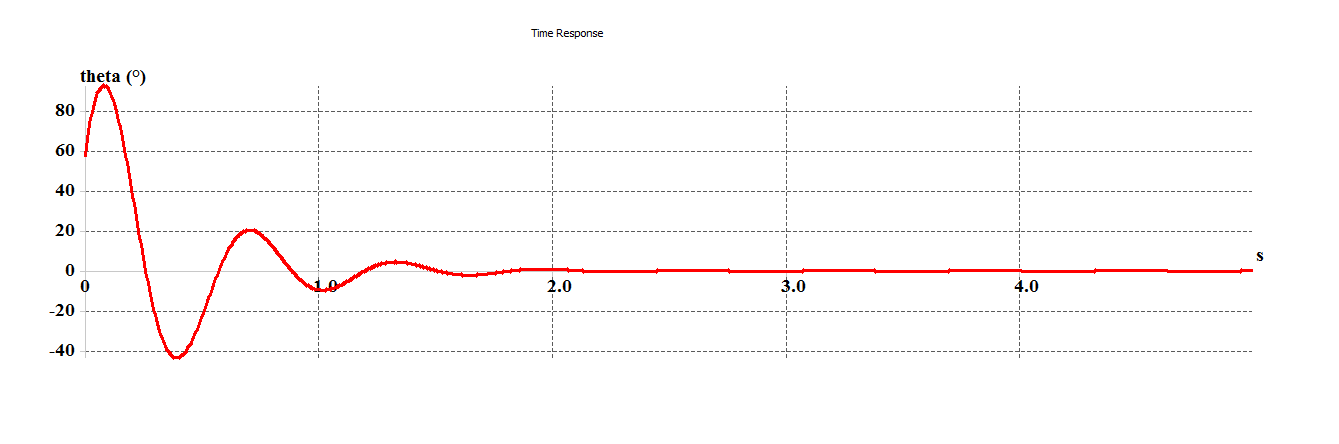
\includegraphics[width = \linewidth]{theta__1_.png}
\end{subfigure}
\caption{Short Period Mode Analysis in First Iteration}
\end{figure}
\subsection{Conclusions from Aerodynamic Analysis}
At 40 degrees of aileron deflection, the CL was reduced significantly and CD saw an increase. \\
Moreover, the trim condition did not correspond to the maxima of CL/CD, which the condition for a cruise state. If this condition is not satisfied, the cruise will be terribly inefficient.\\
Hence, we have decided to reject this configuration.\\

\section{Structural Analysis}
For structural analysis, we have used ANSYS static structural for analysing the strength of material used. 
In our first iteration, teh whole solid body is made up of aluminum alloy which has resulted in a lot of weight.
We have not included any stringers and ribs for our analysis.
\begin{figure}[H]
\begin{subfigure}{0.48\textwidth}
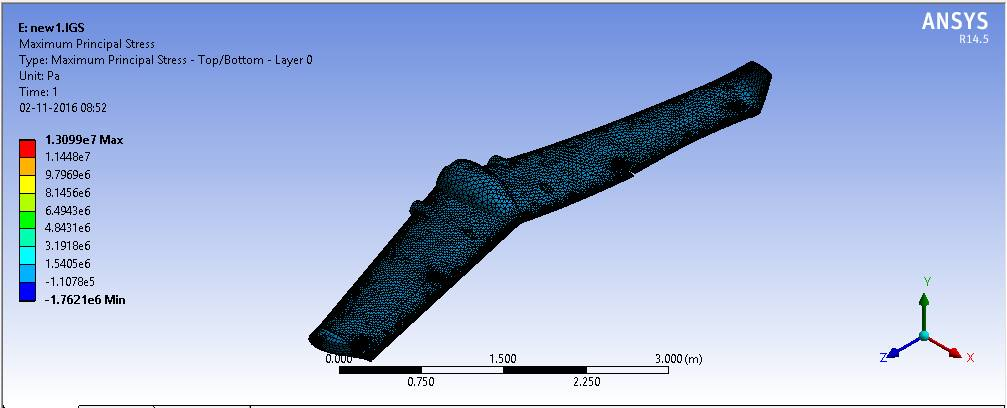
\includegraphics[width = \linewidth]{str1.png}
\end{subfigure}
\begin{subfigure}{0.48\textwidth}
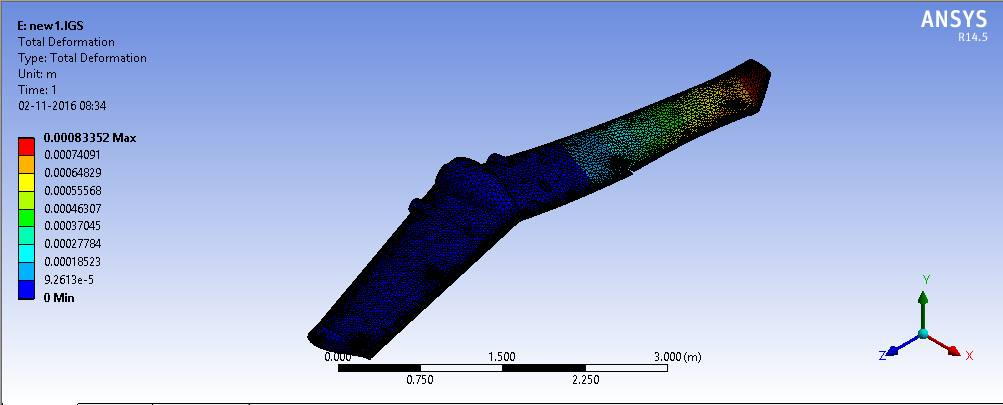
\includegraphics[width = \linewidth]{str2.png}
\end{subfigure}
\end{figure}
\section{Objective Function}
The objective function of our design is the mass of fuel consumed in the journey. Our flight path consists of mainly vertical take-off, cruise and hover. 
In cruise, the mass of fuel consumed is calculated using the range equation, and the amount of fuel consumed has nothing to be optimised much. However, in vertical take-off and hover, the mass of fuel
consumed can be optimised by changing some parameters mainly, the duct diameter, velocity of duct, acceleration of take-off.
From, the above calculations in point performance, we calcuate the toital mass of fuel consumed in the journey comes out to be
$m_f = 5 + 5 + 20 = 30kg $ 
\section{Modifications}
\begin{table}[H]
\begin{center}
\begin{tabular}{ |c| c| c| }
\hline
 Design Variable & Iteration-1 & Iteration-2 \\ 
 \hline
 Span & 4m & 5m \\ 
 \hline
 Taper Ratio & 0.5 & 0.7 \\ 
 \hline
 Position of Aileron & 0.8m from root chord & 1.2m from root chord \\
 \hline
 Size of Aileron & 0.14$m^2$ & 0.3$m^2$ \\
 \hline
 Airfoil & NACA 4412 & MH 60 \\
 \hline
 Placement of Engine & 0.5 from root chord & 0.5 from root chord \\
 \hline
 Volume of Fuselage & 0.12$m^3$ & 0.2$m^3$ \\
 \hline
\end{tabular}
\end{center}
\caption{Modifications}
\end{table}

\chapter{Second Iteration}
\section{CAD Model}
\begin{figure}[H]
\centering
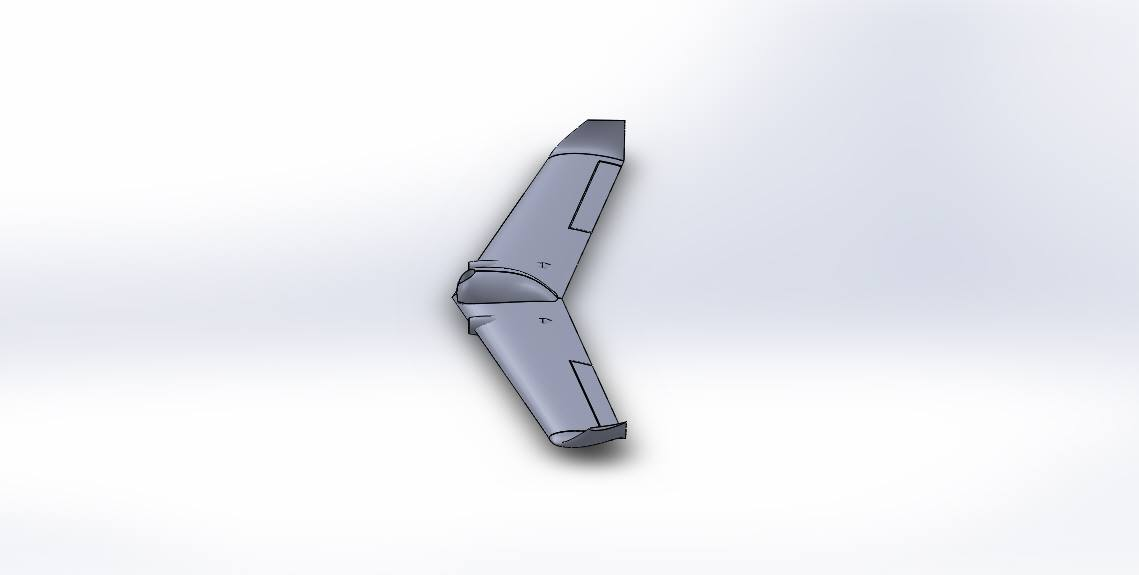
\includegraphics[width = \textwidth]{iter2.jpg}
\caption{CAD Model of iteration2}
\end{figure}

\section{Weight Estimation}
The total estimated weight of the aircraft comes out to be around 135-140kg. The distribution goes as follows.\\
\begin{table}[H]
\begin{center}
\begin{tabular}{ |c| c| }
\hline
 Wing & 90kg \\ 
 Fuselage & 10kg \\ 
 Control Surfaces & 5 Kg \\ 
 Camera & 5kg \\
 Electronics & 5kg \\
 Ejector System & 5kg \\
 Engine & $3\times7.5$kg \\
 Payload & 10kg \\
 Fuel & 60kg \\
 \hline
 Total & 210kg \\
\hline
\end{tabular}
\end{center}
\caption{Weight Estimation in Second Iteration.}
\label{Table2}
\end{table}
Now, we need to calculate thrust required for vertical take-off. \\
We take the acceleration for the take-off to be 0.5$\frac{m}{s^2}$
T = m(g+a) = 210(9.8+0.5) = 2163N \\
%%% Block Diagram%%%
This control block gives the value of $T_1$,$T_2$ based on C.G.
\begin{center}
$M_{cg} = T_1x_{cg1} - 2T_2x_{cg2}$ \\
$T_1x_{cg1} = 2T_2x_{cg2}$ \\
$T_1 + T_2 + T_3 = W$ \\
\end{center}
For vertical take off:
\begin{center}
$d = \frac{1}{2}at^2 \implies 150 = \frac{1}{2}0.5t^2$
t = 25-30s
\end{center}
Hence, assume transition takes place in 20-30 seconds. 
\section{Engine Analysis}
\textbf{Engine Chosen:PBS TJ-40} Given the data from  \url{http://www.pbsvb.com/customer-industries/aerospace/aircraft-engines/tj40-g2-turbojet-engine} \\
$\rho_{air} = 1.225\frac{kg}{m^3}$, $A_C = \frac{\pi d_c^2}{4}$, $\dot{m} = \rho_{air} \times V \times A_C$ \\
$KE_{per mass} = \frac{V^2}{2}$, power = $\dot{m}\times KE_{per mass}$ \\
lift = $\dot{m}V = \rho_{air}\times V\times A_C\times V = \rho_{air}\times V^2 \times \frac{\pi d_c^2}{4}$ \\
$3\dot{m}V_{duct} = m(V_{air} + g) = 210\times 20.3$
\section{Point Performance}
We have 3 main stages in the fight profile namely vertical take-off(VTOF), cruise, hover. We consider transition phase to be negligible, however we carry some extra fuel for that phase. 
\subsection{VTOF}
$m_f = \dot{m_f}\times t = \rho_{fuel}\times A_{duct}\times V \times t$ (t$\sim$60s)
By calculation, we get the mass of fuel consumed comes out to be 5kgs.
\subsection{Cruise}
$R = \frac{V_{cruise}}{C_{cruise}}\times\frac{L}{D}\times0.866 \times ln(\frac{W_{i-1}}{W_i})$ \\
where R is range $V_{cruise}$ is cruise speed, $c_{cruise}$ is the speed of sound in cruise conditions, $\frac{L}{D}$ is lift to drag ratio in cruise conditions and $W_{i-1}, W_i$ are weights before and after the cruise leg respectively.\\
18000 = $\frac{40}{c_{cruise}}\times20\times0.8666\times ln(\frac{W}{W - m_f})$
By calculation, we get the mass of fuel consumed comes out to be 18kgs.
\subsubsection{Hover}
Hover profile is almost same as VTOF, except we don't have vertical acceleration.\\
So, $V_{duct}$ will be lower.\\
Hence, $m_f = \dot{m_f}\times t$, $\dot{m_f}$ will be less.\\
But time t is of the order of 120-150 s. So, fuel consumed is higher.\\
Hence we take fuel(initial) to be twice the total fuel calculated because of the return path.
By calculation, we get the mass of fuel consumed comes out to be 5.5kgs.
\section{Aerodynamic Analysis}
\subsection{Selection of Airfoil}
Due to undesirable moment characteristics that resulted in high aileron deflections, we were compelled to abandon the previous configuration. In order to have low deflections, we decided to opt for self-stable airfoils. In case of a self-stable airfoil, the moment coefficient is positive at zero angle of attack. A negative slope will hence imply a trim condition at a particular angle of attack even without any aileron deflection. It is due to this reason that self-stable airfoils are particularly used in case of a flying wing, due to the lack of a tail for control.\\
We decided to use the self-stable airfoil MH60. Source: \url{http://www.mh-aerotools.de/airfoils/mh60koo.htm}
\subsection{Aerodynamic Plots}
We performed aerodynamic analysis on the plane with modified geometry and new airfoil. We carried out calculations for various aileron deflections, and found that a deflection of 5 degrees resulted in desirable results.\\
The following plots are deduced from the aerodynamic analysis of the aircraft.
\begin{figure}[H]
\begin{subfigure}{0.6\textwidth}
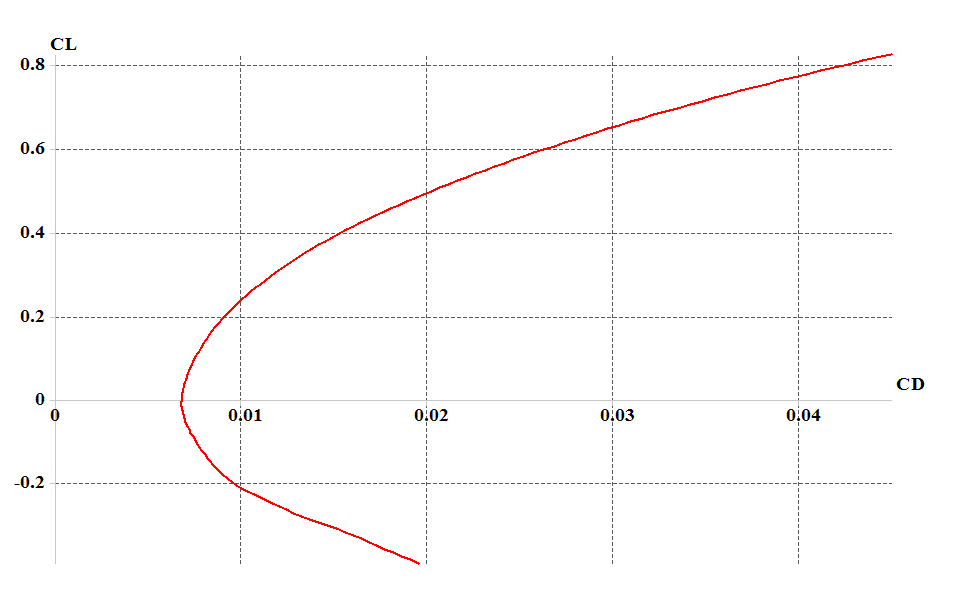
\includegraphics[width = \linewidth]{cl_vs_cd__1_.png}
\caption{$C_l$ vs $C_d$}
\end{subfigure}
\begin{subfigure}{0.6\textwidth}
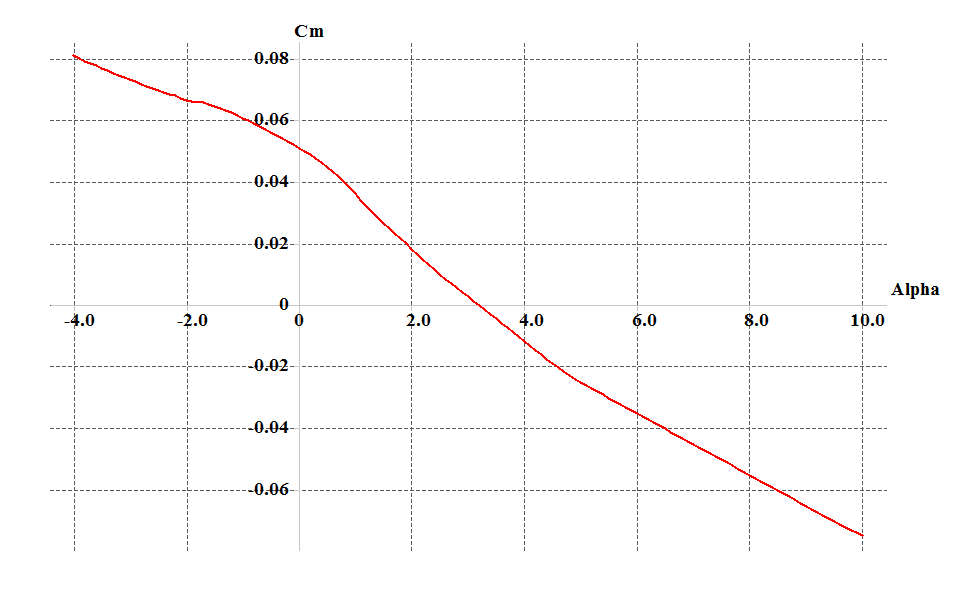
\includegraphics[width = \linewidth]{cm_alpha__1_.png}
\caption{Moment coefficient about Y-axis through C.G. vs $\alpha$}
\end{subfigure}
\medskip
\begin{subfigure}{0.6\textwidth}
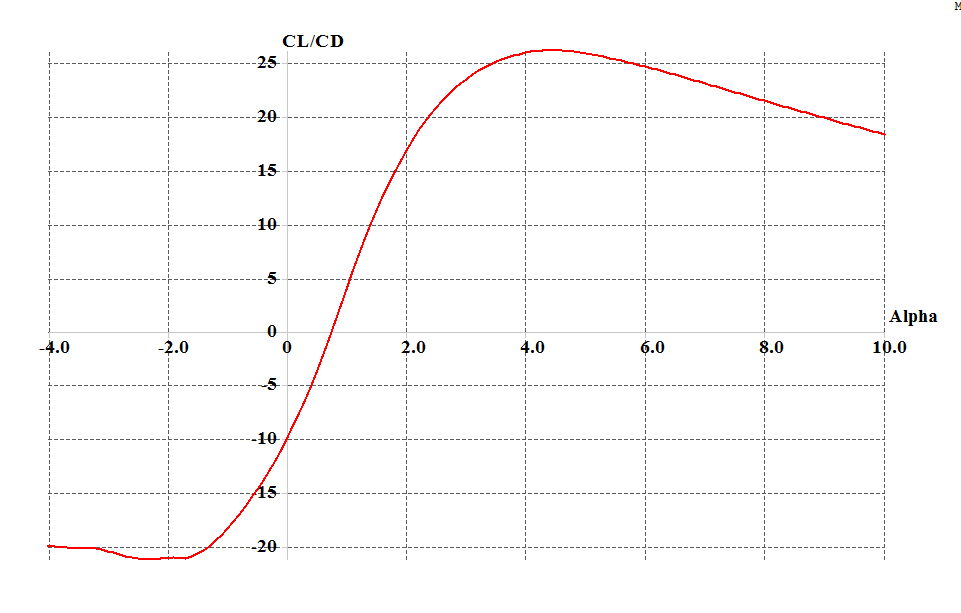
\includegraphics[width = \linewidth]{clcd_vs_alpha__1_.png}
\caption{$\frac{C_l}{C_d}$ vs $\alpha$}
\end{subfigure}
\begin{subfigure}{0.6\textwidth}
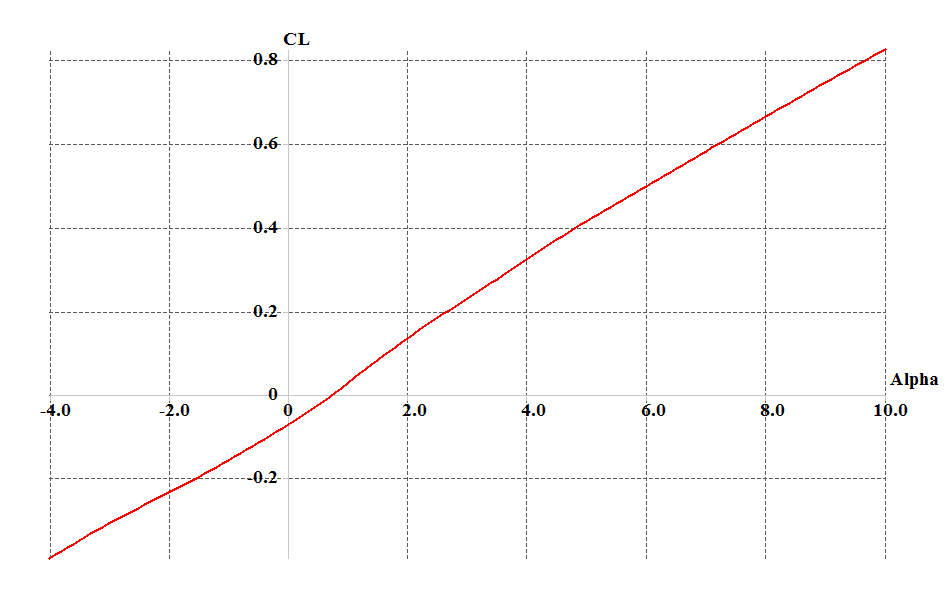
\includegraphics[width = \linewidth]{cl_alpha.png}
\caption{$C_l$ vs $\alpha$}
\end{subfigure}
\caption{Aerodynamic Analysis in Second Iteration}
\end{figure}
\section{Trim Analysis}
For a trim condition, the moment coefficient should be zero. From the above plots, the trim condition occurs at 3.2 degrees of angle of attack. The slope of moment coefficient against angle of attack was found to be negative, fulfilling the condition for longitudinal static stability.\\
At this angle of attack, the $\frac{C_L}{C_D}$ is also close to maximum, hence an efficient cruise condition. This has resulted in the elimination of the second reason why we rejected our first design configuration.\\

\section{Stability Analysis}
At an aileron deflection of 5 degrees, the stability analysis was carried out.
The following are the time response plots of the five modes. The modes are decoupled, which enables us to study each mode in isolation, unlike in a real world scenario where the actual response is the sum of all five modes of instability.
It can be inferred from the above plots that the aircraft is stable in short period mode, phugoid mode and roll subsidence mode. However, the aircraft is visibly unstable in the Dutch Roll mode.

\begin{table}[H]
\begin{center}
\begin{tabular}{ |c| c| c| }
\hline
 Mode & Damping & Frequency(Hz) \\ 
 \hline
 Phugoid Mode & 0.003 & 0.053 \\ 
 \hline
 Short Period & 0.324 & 0.804 \\ 
 %Roll subsidence Mode & 1 & 0 \\
 \hline
 Dutch Roll Mode & -0.119 & 0.213 \\
 %Spiral Mode & 1 & 0 \\
 \hline
\end{tabular}
\end{center}
\caption{Damping and Frequencies for various modes.}
\end{table}
\subsection{Roll Mode}
\begin{figure}[H]
\begin{subfigure}{0.48\textwidth}
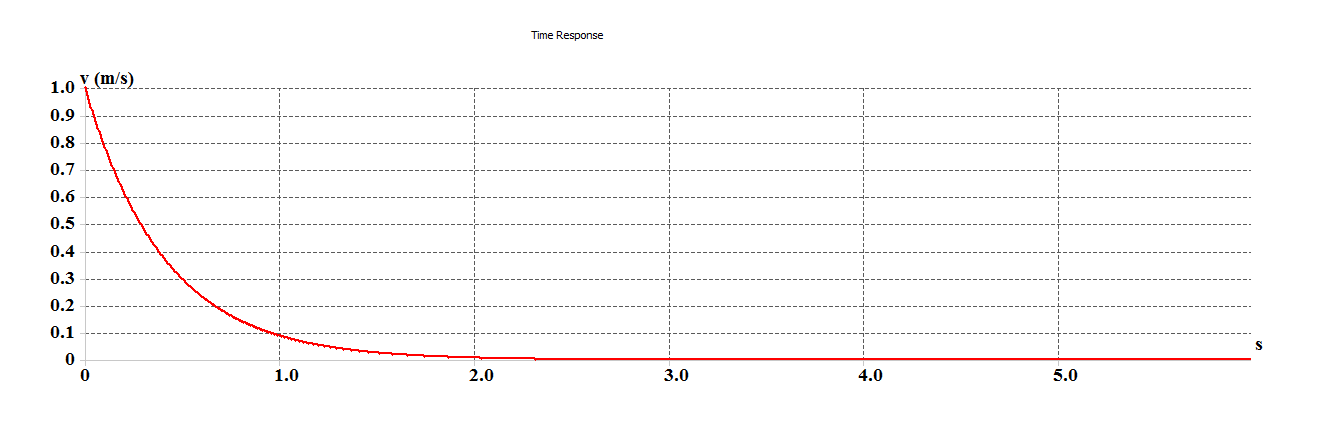
\includegraphics[width = \linewidth]{v__3_.png}
\end{subfigure}
\begin{subfigure}{0.48\textwidth}
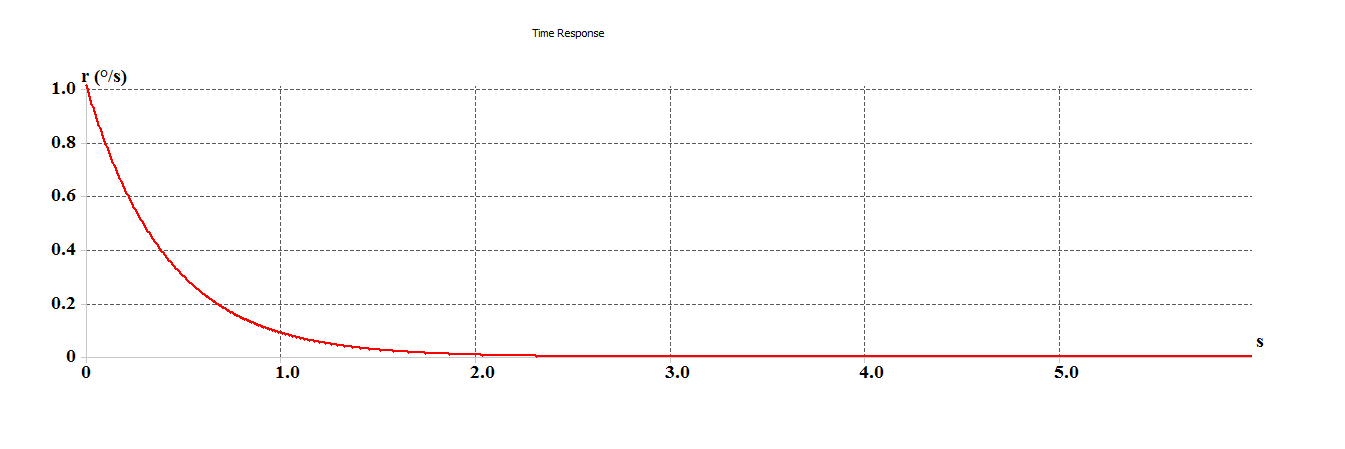
\includegraphics[width = \linewidth]{r__3_.png}
\end{subfigure}
\medskip
\begin{subfigure}{0.48\textwidth}
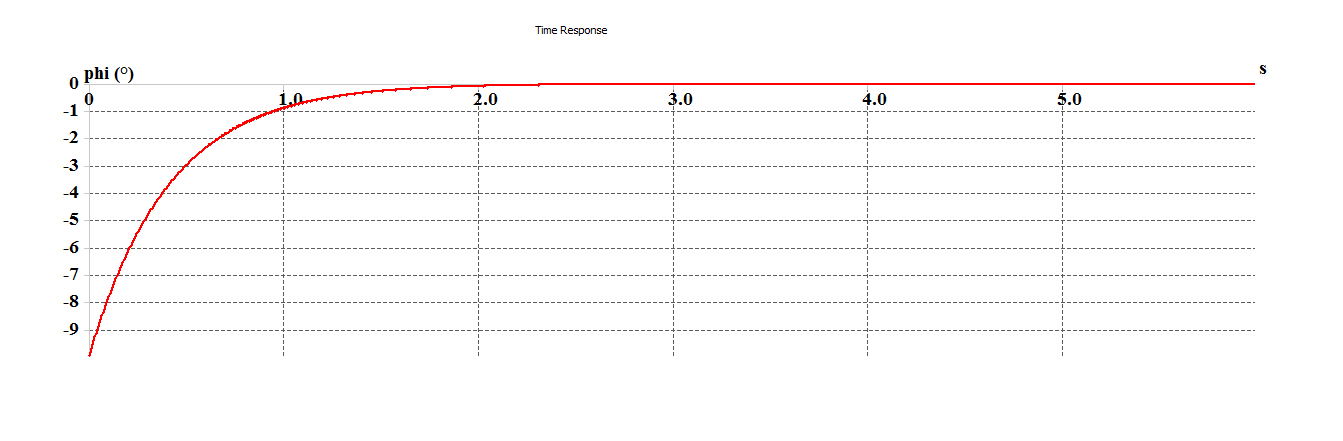
\includegraphics[width = \linewidth]{phi__3_.png}
\end{subfigure}
\begin{subfigure}{0.48\textwidth}
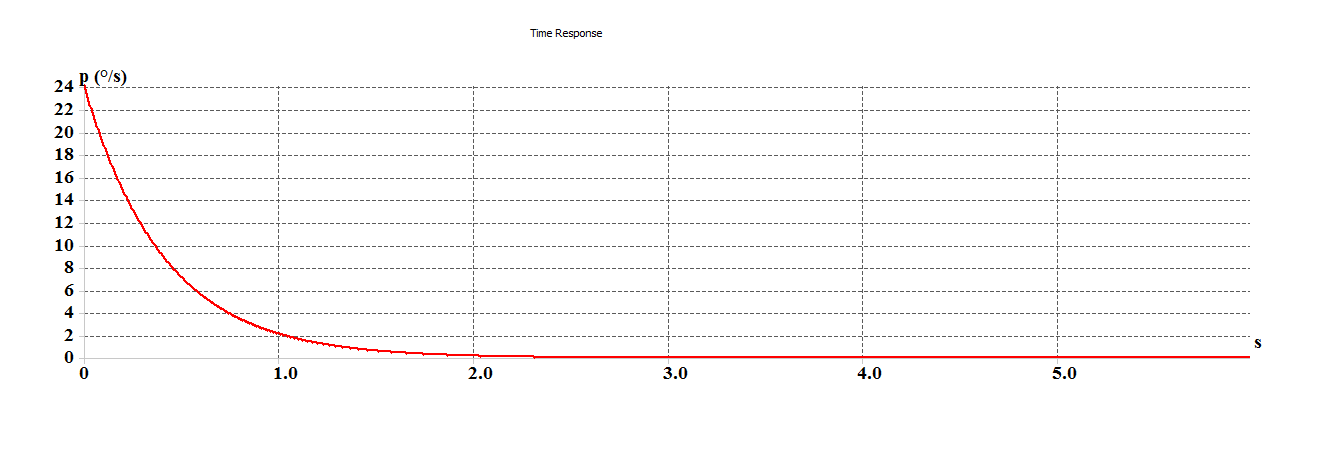
\includegraphics[width = \linewidth]{p__3_.png}
\end{subfigure}
\caption{Roll Mode Analysis in Second Iteration}
\end{figure}
\subsection{Phugoid Mode}
\begin{figure}[H]
\begin{subfigure}{0.48\textwidth}
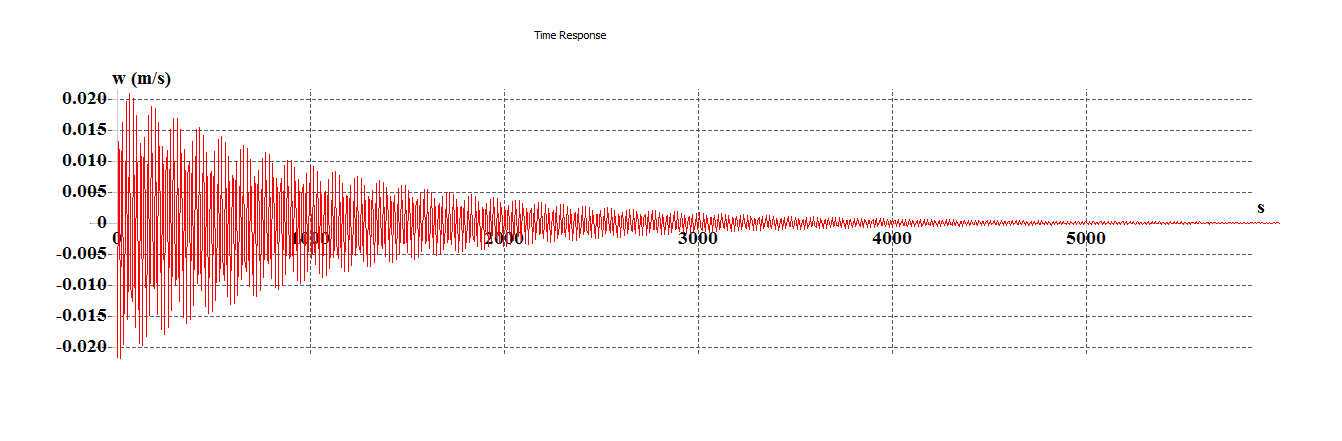
\includegraphics[width = \linewidth]{w__3_.png}
\end{subfigure}
\begin{subfigure}{0.48\textwidth}
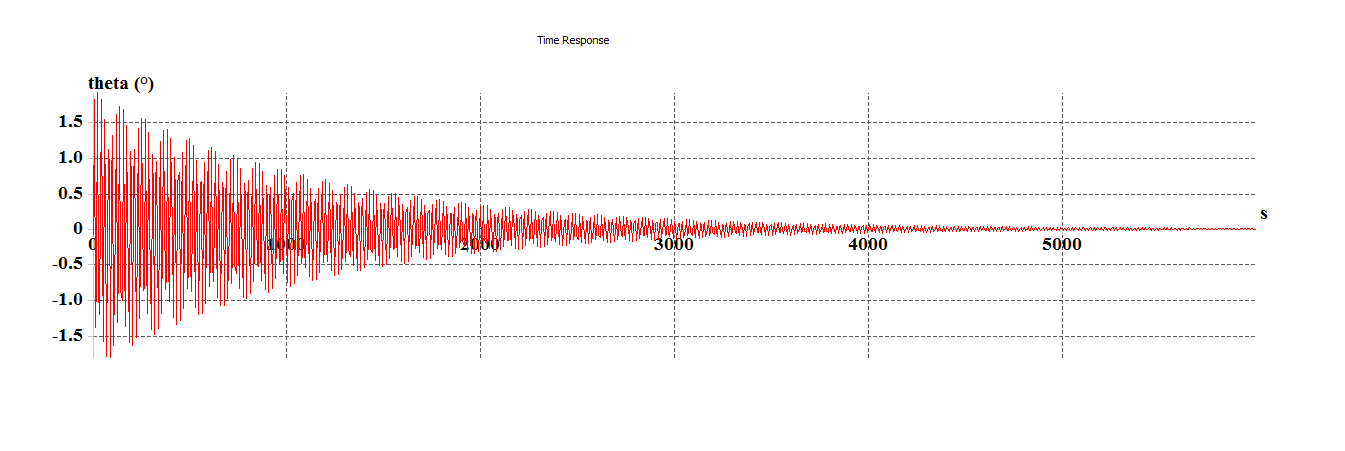
\includegraphics[width = \linewidth]{theta__3_.png}
\end{subfigure}
\medskip
\begin{subfigure}{0.48\textwidth}
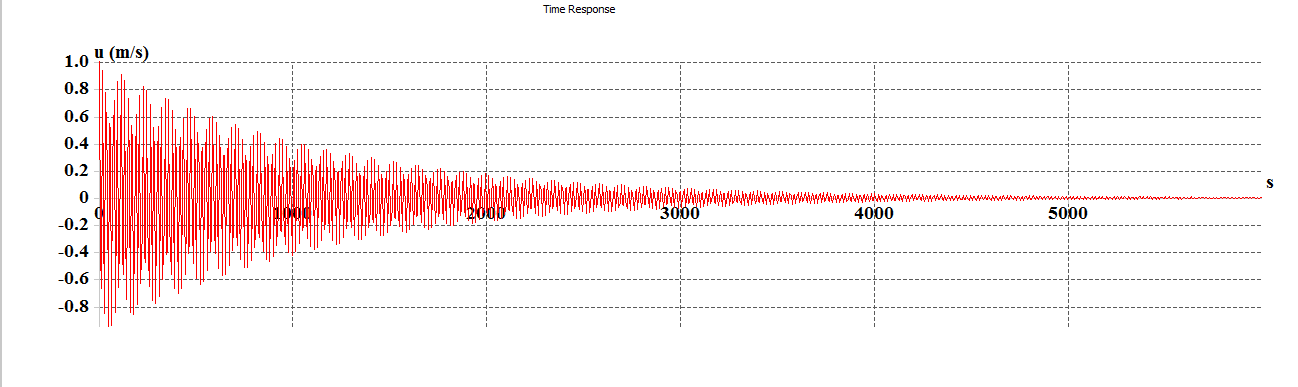
\includegraphics[width = \linewidth]{u__3_.png}
\end{subfigure}
\begin{subfigure}{0.48\textwidth}
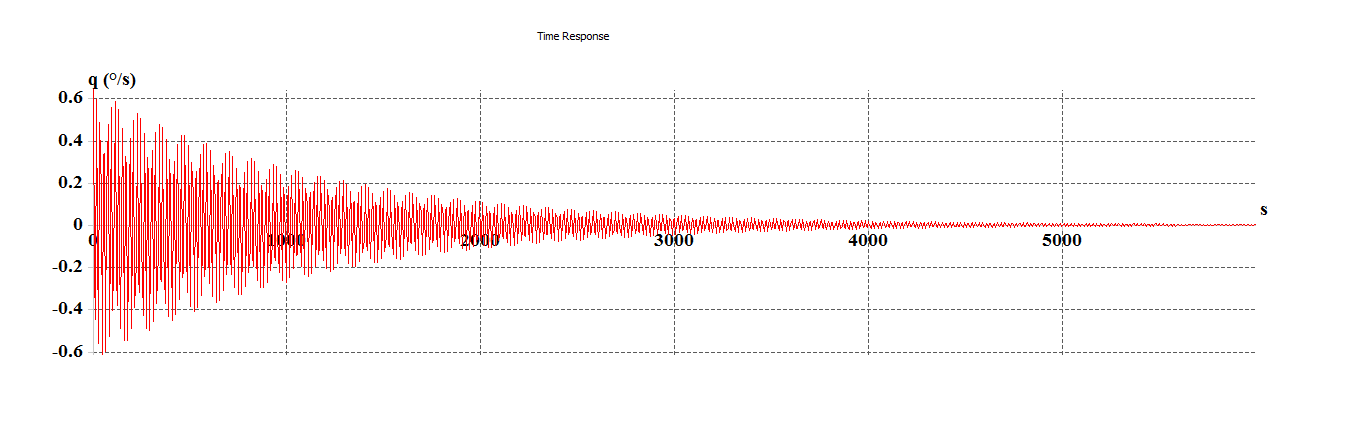
\includegraphics[width = \linewidth]{q__3_.png}
\end{subfigure}
\caption{Phugoid Mode Analysis in Second Iteration}
\end{figure}
\subsection{Dutch Roll Mode}
\begin{figure}[H]
\begin{subfigure}{0.48\textwidth}
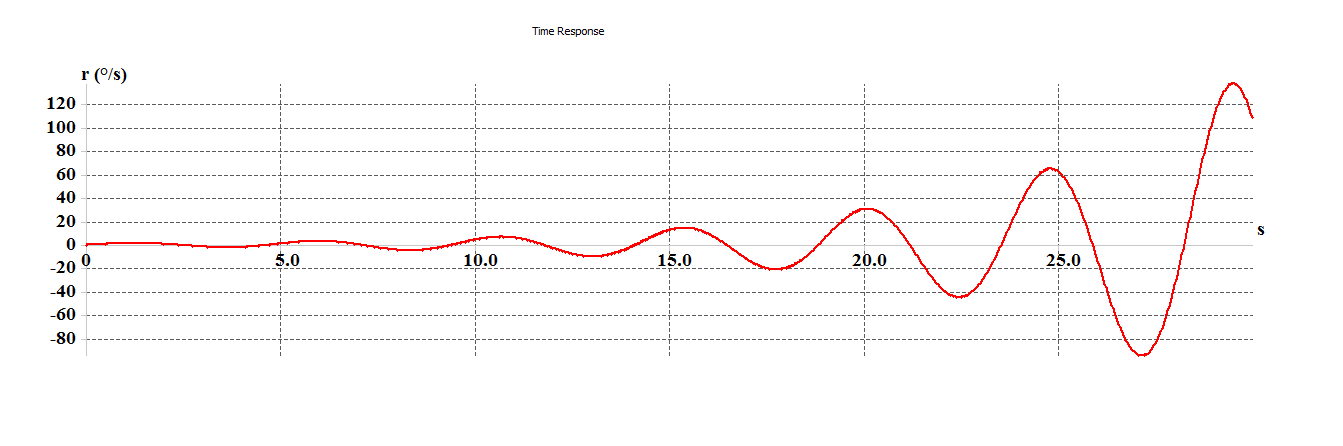
\includegraphics[width = \linewidth]{r__5_.png}
\end{subfigure}
\begin{subfigure}{0.48\textwidth}
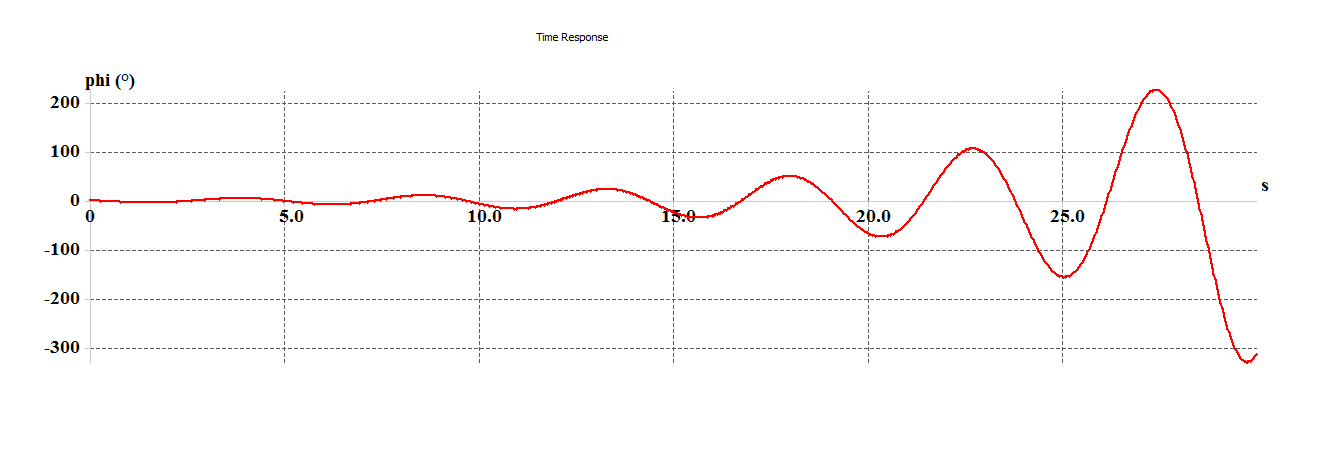
\includegraphics[width = \linewidth]{phi__5_.png}
\end{subfigure}
\medskip
\begin{subfigure}{0.48\textwidth}
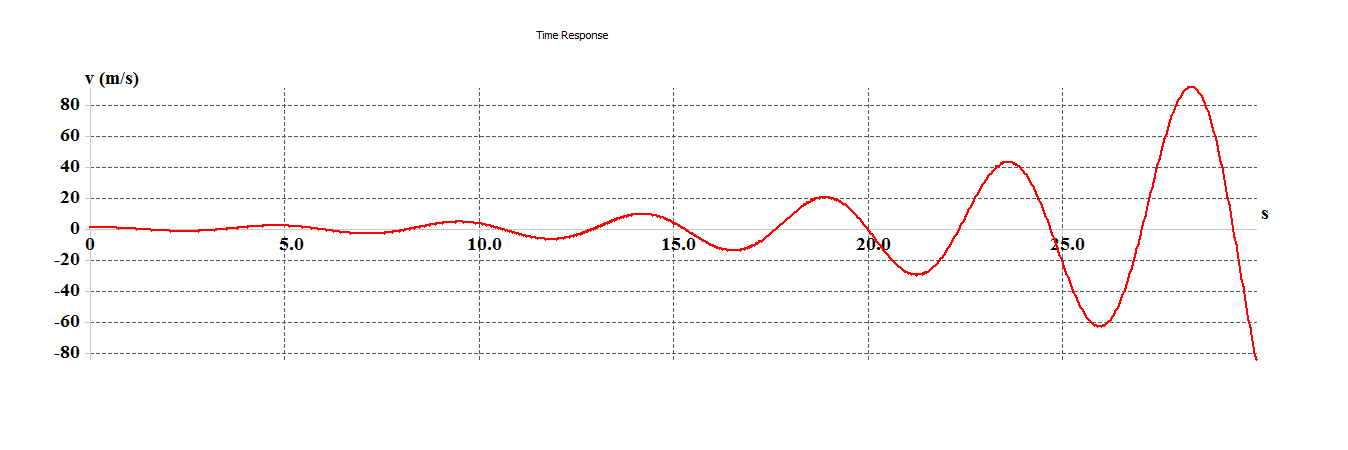
\includegraphics[width = \linewidth]{v__5_.png}
\end{subfigure}
\begin{subfigure}{0.48\textwidth}
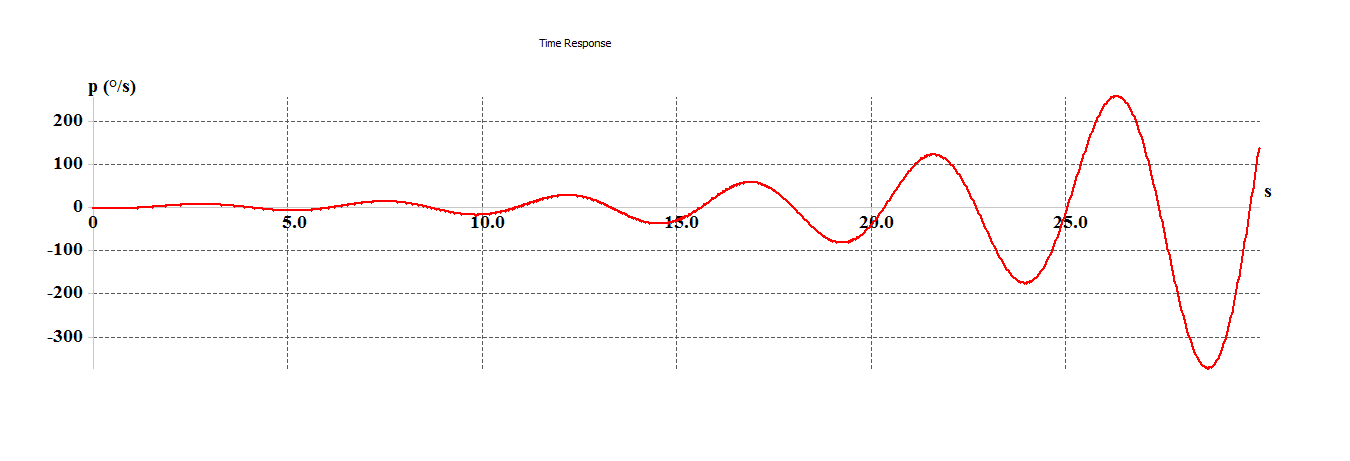
\includegraphics[width = \linewidth]{p__5_.png}
\end{subfigure}
\caption{Dutch Roll Mode Analysis in Second Iteration}
\end{figure}
\subsection{Spiral Mode}
\begin{figure}[H]
\begin{subfigure}{0.48\textwidth}
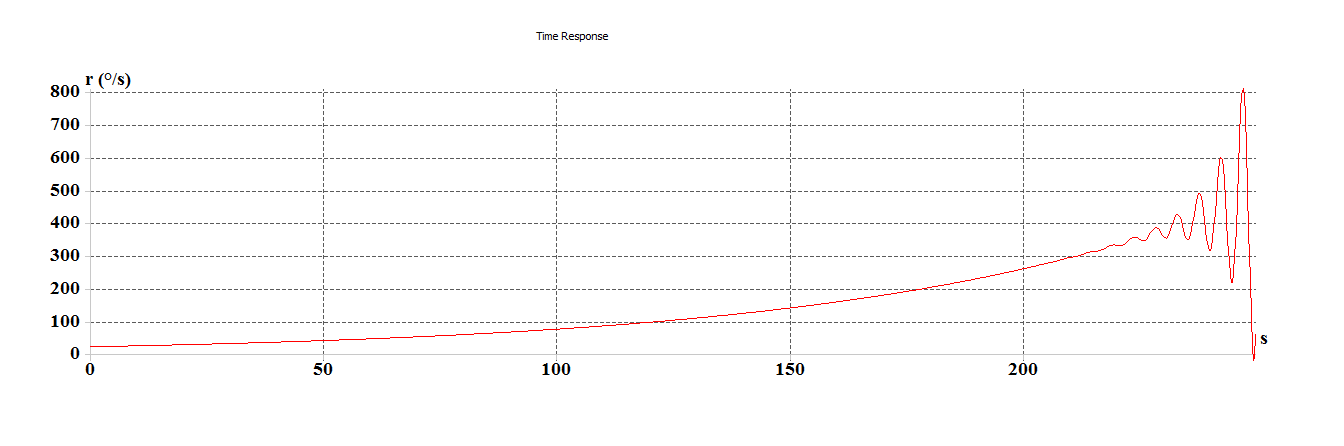
\includegraphics[width = \linewidth]{r__4_.png}
\end{subfigure}
\begin{subfigure}{0.48\textwidth}
\includegraphics[width = \linewidth]{v__4_.png}
\end{subfigure}
\medskip
\begin{subfigure}{0.48\textwidth}
\includegraphics[width = \linewidth]{phi__4_.png}
\end{subfigure}
\begin{subfigure}{0.48\textwidth}
\includegraphics[width = \linewidth]{p__4_.png}
\end{subfigure}
\caption{Spiral Mode Analysis in Second Iteration}
\end{figure}
\subsection{Short Period Mode}
\begin{figure}[H]
\begin{subfigure}{0.48\textwidth}
\includegraphics[width = \linewidth]{w__2_.png}
\end{subfigure}
\begin{subfigure}{0.48\textwidth}
\includegraphics[width = \linewidth]{u__2_.png}
\end{subfigure}
\medskip
\begin{subfigure}{0.48\textwidth}
\includegraphics[width = \linewidth]{q__2_.png}
\end{subfigure}
\begin{subfigure}{0.48\textwidth}
\includegraphics[width = \linewidth]{theta__2_.png}
\end{subfigure}
\caption{Short Period Mode Analysis in Second Iteration}
\end{figure}
\subsection{Conclusions from Aerodynamic Analysis}
We were able to eliminate our two objections from the previous iteration, as our aircraft is trimmed at a low aileron deflection and satisfies cruise conditions.\\
However, the aircraft was found to be unstable in the Dutch Roll mode. Due to this, we cannot accept the present configuration.
\\
Moreover, the lift generated at trim condition was not sufficient enough to carry the weight of the aircraft.
\\
Hence, we have decided to reject this configuration and rectify the above two impairments for our next configuration.
\\
\section{Structural Analysis}
In this second iteration, we have used ANSYS static structural for analysing the material used. The following plots show the stress and strain variations along the span of the wing.
However, we have not used any stringers and ribs in our analysis, which we  have incorporated in our next iteration.
\begin{figure}[H]
\begin{subfigure}{0.48\textwidth}
\includegraphics[width = \linewidth]{iter2_mesh.png}
\end{subfigure}
\begin{subfigure}{0.48\textwidth}
\includegraphics[width = \linewidth]{iter2_tot_def.png}
\end{subfigure}
\medskip
\begin{subfigure}{0.48\textwidth}
\includegraphics[width = \linewidth]{iter2_max_stress.png}
\end{subfigure}
\begin{subfigure}{0.48\textwidth}
\includegraphics[width = \linewidth]{iter2_max_strain.png}
\end{subfigure}
\caption{Structural Analysis in Second Iteration}
\end{figure}
\section{Objective Function}
The objective function of our design is the mass of fuel consumed in the journey. Our flight path consists of mainly vertical take-off, cruise and hover. 
In cruise, the mass of fuel consumed is calculated using the range equation, and the amount of fuel consumed has nothing to be optimised much. However, in vertical take-off and hover, the mass of fuel
consumed can be optimised by changing some parameters mainly, the duct diameter, velocity of duct, acceleration of take-off.
From, the above calculations in point performance, we calcuate the toital mass of fuel consumed in the journey comes out to be
$m_f = 5kg + 5kg + 5kg = 15kg $ 
\section{Modifications}
\begin{table}[H]
\begin{center}
\begin{tabular}{ |c| c| c| }
\hline
 Design Variable & Iteration-2 & Iteration-3 \\ 
 \hline
 Span & 5m & 5m \\ 
 \hline
 Taper Ratio & 0.7 & 0.8 \\ 
 \hline
 Position of Aileron & 1.2m from root chord & 1.2m from root chord \\
 \hline
 Size of Aileron & 0.3$m^2$ & 0.3$m^2$ \\
 \hline
 Airfoil & MH 60 & HS 130 \\
 \hline
 Placement of Engine & 0.5 from root chord & 0.5 from root chord \\
 \hline
 Wing Tip & 0.25m$\times$0.5m & 0.3m$\times$0.5m \\
 \hline
\end{tabular}
\end{center}
\caption{Modifications}
\end{table}

\chapter{Third Iteration}
\section{CAD Model}
\begin{figure}[H]
\centering
\includegraphics[width = \textwidth]{iter3-2.png}
\caption{CAD Model of iteration3}
\end{figure}
\begin{figure}[H]
 \centering
 \includegraphics[width = 1.4\textwidth]{iter3.png}
 \caption{Dimensions of Iteration3}
\end{figure}
\newpage
\section{Weight Estimation}
The total estimated weight of the aircraft comes out to be around 135-140kg. The distribution goes as follows.\\
\begin{table}[H]
\begin{center}
\begin{tabular}{ |c| c| }
\hline
 Wing & 56kg \\ 
 Fuselage & 10kg \\ 
 Control Surfaces & 5 Kg \\ 
 Camera & 5kg \\
 Electronics & 5kg \\
 Ejector System & 5kg \\
 Engine & $3\times7.5$kg \\
 Payload & 10kg \\
 Fuel & 30kg \\
 \hline
 Total & 140kg \\
\hline
\end{tabular}
\end{center}
\caption{Weight Estimation in Third Iteration.}
\label{Table3}
\end{table}
Now, we need to calculate thrust required for vertical take-off. \\
We take the acceleration for the take-off to be 0.5$\frac{m}{s^2}$
T = m(g+a) = 140(9.8+0.5) = 1442N \\
%%% Block Diagram%%%
This control block gives the value of $T_1$,$T_2$ based on C.G.
\begin{center}
$M_{cg} = T_1x_{cg1} - 2T_2x_{cg2}$ \\
$T_1x_{cg1} = 2T_2x_{cg2}$ \\
$T_1 + T_2 + T_3 = W$ \\
\end{center}
For vertical take off:
\begin{center}
$d = \frac{1}{2}at^2 \implies 150 = \frac{1}{2}0.5t^2$
t = 25-30s
\end{center}
Hence, assume transition takes place in 20-30 seconds. 
\section{Engine Analysis}
\textbf{Engine Chosen:PBS TJ-40} Given the data from  \url{http://www.pbsvb.com/customer-industries/aerospace/aircraft-engines/tj40-g2-turbojet-engine} \\
$\rho_{air} = 1.225\frac{kg}{m^3}$, $A_C = \frac{\pi d_c^2}{4}$, $\dot{m} = \rho_{air} \times V \times A_C$ \\
$KE_{per mass} = \frac{V^2}{2}$, power = $\dot{m}\times KE_{per mass}$ \\
lift = $\dot{m}V = \rho_{air}\times V\times A_C\times V = \rho_{air}\times V^2 \times \frac{\pi d_c^2}{4}$ \\
$3\dot{m}V_{duct} = m(V_{air} + g) = 140\times 20.3$
\section{Point Performance}
We have 3 main stages in the fight profile namely vertical take-off(VTOF), cruise, hover. We consider transition phase to be negligible, however we carry some extra fuel for that phase. 
\subsection{VTOF}
$m_f = \dot{m_f}\times t = \rho_{fuel}\times A_{duct}\times V \times t$ (t$\sim$60s)
By calculation, we get the mass of fuel consumed comes out to be 2.5kgs.
\subsection{Cruise}
$R = \frac{V_{cruise}}{C_{cruise}}\times\frac{L}{D}\times0.866 \times ln(\frac{W_{i-1}}{W_i})$ \\
where R is range $V_{cruise}$ is cruise speed, $c_{cruise}$ is the speed of sound in cruise conditions, $\frac{L}{D}$ is lift to drag ratio in cruise conditions and $W_{i-1}, W_i$ are weights before and after the cruise leg respectively.\\
18000 = $\frac{40}{c_{cruise}}\times20\times0.8666\times ln(\frac{W}{W - m_f})$
By calculation, we get the mass of fuel consumed comes out to be 3kgs.
\subsubsection{Hover}
Hover profile is almost same as VTOF, except we don't have vertical acceleration.\\
So, $V_{duct}$ will be lower.\\
Hence, $m_f = \dot{m_f}\times t$, $\dot{m_f}$ will be less.\\
But time t is of the order of 120-150 s. So, fuel consumed is higher.\\
Hence we take fuel(initial) to be twice the total fuel calculated because of the return path.
By calculation, we get the mass of fuel consumed comes out to be 3kgs.
\section{Aerodynamic Analysis}
\subsection{Change of Airfoil}
We decided to change the airfoil as the previous airfoil was not generating enough lift. We found an airfoil called HS130 which had better lift coefficient characteristics. It also had a higher moment coefficient at zero angle of attack.\\
\subsection{Aerodynamic Plots}
After performing analysis on numerous aileron deflections, we came to the conclusion that the deflection of 5 degrees gave reasonable results.\\
The following plots are deduced from the aerodynamic analysis of the aircraft.
\begin{figure}[H]
\begin{subfigure}{0.6\textwidth}
\includegraphics[width = \linewidth]{cl_vs_cd__2_.png}
\caption{$C_l$ vs $C_d$}
\end{subfigure}
\begin{subfigure}{0.6\textwidth}
\includegraphics[width = \linewidth]{cm_alpha__2_.png}
\caption{Moment coefficient about Y-axis through C.G. vs $\alpha$}
\end{subfigure}
\medskip
\begin{subfigure}{0.6\textwidth}
\includegraphics[width = \linewidth]{clcd_vs_alpha__2_.png}
\caption{$\frac{C_l}{C_d}$ vs $\alpha$}
\end{subfigure}
\begin{subfigure}{0.6\textwidth}
\includegraphics[width = \linewidth]{cl_vs_alpha__1_.png}
\caption{$C_l$ vs $\alpha$}
\end{subfigure}
\caption{Aerodynamic Analysis in Third Iteration}
\end{figure}
\section{Trim Analysis}
The trim condition was found to be at angle of attack 4.6 degrees. At this angle of attack, the CL/CD is also close to maximum, hence fulfilling our cruise conditions.\\
The slope of moment coefficient against angle of attack was found to be negative, fulfilling the condition for longitudinal static stability.\\

\section{Stability Analysis}
The stability analysis was carried out at a deflection of 5 degrees and angle of attack 4.6 degrees, the trim condition.\\
The following are the time response plots of the five modes. The modes are decoupled, which enables us to study each mode in isolation, unlike in a real world scenario where the actual response is the sum of all five modes of instability.\\
It can be inferred from the above plot that the aircraft is stable in all modes. The short period, dutch roll and roll subsidence modes are highly damped. The phugoid mode is also relatively highly damped. Spiral Mode is lightly damped.\\

\begin{table}[H]
\begin{center}
\begin{tabular}{ |c| c| c| }
\hline
 Mode & Damping & Frequency(Hz) \\ 
 \hline
 Phugoid Mode & 0.101 & 0.051 \\ 
 \hline
 Short Period & 0.277 & 3.266 \\ 
 %Roll subsidence Mode & 1 & 0 \\
 \hline
 Dutch Roll Mode & 0.243 & 0.344 \\
 %Spiral Mode & 1 & 0 \\
 \hline
\end{tabular}
\end{center}
\caption{Damping and Frequencies for various modes.}
\end{table}
\subsection{Roll Mode}
\begin{figure}[H]
\begin{subfigure}{0.48\textwidth}
\includegraphics[width = \linewidth]{v (1).png}
\end{subfigure}
\begin{subfigure}{0.48\textwidth}
\includegraphics[width = \linewidth]{r (1).png}
\end{subfigure}
\medskip
\begin{subfigure}{0.48\textwidth}
\includegraphics[width = \linewidth]{phi (1).png}
\end{subfigure}
\begin{subfigure}{0.48\textwidth}
\includegraphics[width = \linewidth]{p (1).png}
\end{subfigure}
\caption{Roll Mode Analysis in Third Iteration}
\end{figure}
\subsection{Phugoid Mode}
\begin{figure}[H]
\begin{subfigure}{0.48\textwidth}
\includegraphics[width = \linewidth]{w (1).png}
\end{subfigure}
\begin{subfigure}{0.48\textwidth}
\includegraphics[width = \linewidth]{theta (1).png}
\end{subfigure}
\medskip
\begin{subfigure}{0.48\textwidth}
\includegraphics[width = \linewidth]{u (1).png}
\end{subfigure}
\begin{subfigure}{0.48\textwidth}
\includegraphics[width = \linewidth]{q (1).png}
\end{subfigure}
\caption{Phugoid Mode Analysis in Third Iteration}
\end{figure}
\subsection{Dutch Roll Mode}
\begin{figure}[H]
\begin{subfigure}{0.48\textwidth}
\includegraphics[width = \linewidth]{r (2).png}
\end{subfigure}
\begin{subfigure}{0.48\textwidth}
\includegraphics[width = \linewidth]{phi (2).png}
\end{subfigure}
\medskip
\begin{subfigure}{0.48\textwidth}
\includegraphics[width = \linewidth]{v (2).png}
\end{subfigure}
\begin{subfigure}{0.48\textwidth}
\includegraphics[width = \linewidth]{p (2).png}
\end{subfigure}
\caption{Dutch Roll Mode Analysis in Third Iteration}
\end{figure}
\subsection{Spiral Mode}
\begin{figure}[H]
\begin{subfigure}{0.48\textwidth}
\includegraphics[width = \linewidth]{r (3).png}
\end{subfigure}
\begin{subfigure}{0.48\textwidth}
\includegraphics[width = \linewidth]{v (3).png}
\end{subfigure}
\medskip
\begin{subfigure}{0.48\textwidth}
\includegraphics[width = \linewidth]{phi (3).png}
\end{subfigure}
\begin{subfigure}{0.48\textwidth}
\includegraphics[width = \linewidth]{p (3).png}
\end{subfigure}
\caption{Spiral Mode Analysis in Third Iteration}
\end{figure}
\subsection{Short Period Mode}
\begin{figure}[H]
\begin{subfigure}{0.48\textwidth}
\includegraphics[width = \linewidth]{w (2).png}
\end{subfigure}
\begin{subfigure}{0.48\textwidth}
\includegraphics[width = \linewidth]{u (2).png}
\end{subfigure}
\medskip
\begin{subfigure}{0.48\textwidth}
\includegraphics[width = \linewidth]{q (2).png}
\end{subfigure}
\begin{subfigure}{0.48\textwidth}
\includegraphics[width = \linewidth]{theta (2).png}
\end{subfigure}
\caption{Short Period Mode Analysis in Third Iteration}
\end{figure}
\section{Objective Function}
The objective function of our design is the mass of fuel consumed in the journey. Our flight path consists of mainly vertical take-off, cruise and hover. 
In cruise, the mass of fuel consumed is calculated using the range equation, and the amount of fuel consumed has nothing to be optimised much. However, in vertical take-off and hover, the mass of fuel
consumed can be optimised by changing some parameters mainly, the duct diameter, velocity of duct, acceleration of take-off.
From, the above calculations in point performance, we calcuate the toital mass of fuel consumed in the journey comes out to be
$m_f = 3 + 2.5 +3 = 8.5kg $ 
\chapter{Advantages and Limitations}
The final desgin so designed by performing aerodynamic analysis, structural analysis, stability and trim analysis is capable enough to meet all the specifications 
of the mission statement. However any design can be improved at any stage. Similarly, our design at the current status has a lot of positives and negatives also: \\
\textbf{Advantages}:
\begin{enumerate}
 \item Reaches the hazard site quickly.
 \item Travel at large heights.
\end{enumerate}
\textbf{Limitations}:
\begin{enumerate}
 \item Low payload carrying capacity.
 \item Restricted to Class A fires.
\end{enumerate}

\chapter{Future Potential}
The design thus arrived upon can be improved by many ways.  \\
The first area of possible future development is automation. Following just a signal from the operator, the aircraft could be programmed to take off, achieve trim condition appropriately and reach the destination all by itself. The aircraft will be fed the coordinates of the disaster affected point and it will reach it within stipulated time.\\
Another area for automation is the deployment of the aircraft. Any disaster call will immediately result in the aircraft launching itself and reaching the site, effectively eliminating any intermediate human connection. It will reduce the delay due to human inefficiency.\\
Further, the act of dousing the fire can also be automated by appropriate use of heat sensors and algorithms devised for efficient extinguishing of the fire.\\
This aircraft is limited to Class A fires. This constraint can be removed by using better extinguishers and using different building materials.\\
\chapter{Conclusion}
In the above three iterations the main focus was aerodynamics and structures. The choice of flying wing has pushed us to focus on self stable airfoils. We have looked into two such airfoils but there are many such airfoils out there which can better the aerodynamics. But the chosen airfoils improved the trim Cl of overall aircraft from iteration 1 to 3. Also, there was improvement in stability of various vibration modes. Coming to structures, we have moved on from solid interiors to ribs and stringers across iterations, thereby reducing weight drastically.
\begin{thebibliography}{1}

  \bibitem{notes} Modal analysis and experimental
validation {\url{http://www.xflr5.com/docs/XFLR5_Mode_Measurements.pdf}}

  \bibitem{impj}  About XFLR5 calculations and
experimental measurements {\url{http://www.xflr5.com/docs/Results_vs_Prediction.pdf}} 

%%%
  %\bibitem{norman} E. H. Norman {\em Japan's emergence as a modern
  %state} 1940: International Secretariat, Institute of Pacific
  %Relations.

  %\bibitem{fo} Bob Tadashi Wakabayashi {\em Anti-Foreignism and Western
  %Learning in Early-Modern Japan} 1986: Harvard University Press.

\end{thebibliography}
\end{document} to your LaTeX file where you want your
% title page.
%
%%%%%%%%%%%%%%%%%%%%%%%%%%%%%%%%%%%%%%%%%
%\title{Title page with logo}
%----------------------------------------------------------------------------------------
%	PACKAGES AND OTHER DOCUMENT CONFIGURATIONS
%----------------------------------------------------------------------------------------

\documentclass[12pt]{report}
\usepackage[english]{babel}
\usepackage[utf8x]{inputenc}
\usepackage{amsmath}
\usepackage{tikz}
\usetikzlibrary{shapes.geometric,arrows}
\tikzstyle{startstop} = [rectangle, rounded corners, minimum width=3cm, minimum height=1cm,text centered, draw=black, fill=red!30]
\tikzstyle{io} = [trapezium, trapezium left angle=70, trapezium right angle=110, minimum width=3cm, minimum height=1cm, text centered, draw=black, fill=blue!30]
\usepackage{graphicx}
\tikzstyle{process} = [rectangle, minimum width=3cm, minimum height=1cm, text centered, draw=black, fill=orange!30]
\tikzstyle{decision} = [diamond, minimum width=3cm, minimum height=1cm, text centered, draw=black, fill=green!30]
\tikzstyle{arrow} = [thick,->,>=stealth]
\usepackage[colorinlistoftodos]{todonotes}
\usepackage{float}
\usepackage{hyperref}
\usepackage{subcaption}
\begin{document}

\begin{titlepage}

\newcommand{\HRule}{\rule{\linewidth}{0.5mm}} % Defines a new command for the horizontal lines, change thickness here

\center % Center everything on the page
 
%----------------------------------------------------------------------------------------
%	HEADING SECTIONS
%----------------------------------------------------------------------------------------
\textsc{\Large AE 417}\\[0.5cm] % Major heading such as course name
\textsc{\large Aircraft Design Lab}\\[0.5cm] % Minor heading such as course title

%----------------------------------------------------------------------------------------
%	TITLE SECTION
%----------------------------------------------------------------------------------------

\HRule \\[0.4cm]
{ \huge \bfseries Aerial Fire Fighter}\\[0.4cm] % Title of your document
\HRule \\[1.5cm]
 
%----------------------------------------------------------------------------------------
%	AUTHOR SECTION
%----------------------------------------------------------------------------------------

\begin{minipage}{0.4\textwidth}
\begin{flushleft} \large
\emph{Designed by:}\\
Mrinalgouda Patil\\
Rushi Lotti\\ % Your name
Shubham Shinde\\
Veda Krishna Vyas\\
Vikas Kurapati\\
Yashasree Vanam\\
\end{flushleft}
\end{minipage}
~
\begin{minipage}{0.4\textwidth}
\begin{flushright} \large
\emph{Under the guidance of:} \\
Dr. Gopal Shevare\\
Dr. Avijit Chatterjee \\
Dr. Arya Hemendra\\
Dr. Ashok Joshi\\
\end{flushright}
\end{minipage}\\[2cm]

% If you don't want a supervisor, uncomment the two lines below and remove the section above
%\Large \emph{Author:}\\
%John \textsc{Smith}\\[3cm] % Your name

%----------------------------------------------------------------------------------------
%	DATE SECTION
%----------------------------------------------------------------------------------------

%{\large \today}\\[2cm] % Date, change the \today to a set date if you want to be precise

%----------------------------------------------------------------------------------------
%	LOGO SECTION
%----------------------------------------------------------------------------------------

\includegraphics[scale = 0.20]{iitblogo.png} % Include a department/university logo - this will require the graphicx package
 
%----------------------------------------------------------------------------------------

\vfill % Fill the rest of the page with whitespace

\end{titlepage}
\tableofcontents
\newpage
\listoffigures
\newpage
\listoftables

\begin{abstract}
This report deals with the conceptual design of an Unmanned Aerial Vehicle designed to extinguish fires in an urban environment. The problem dictates the travel time and constrains the overall size. A flying wing configuration was chosen from two possible configurations. The ability of vertical take-off and landing were envisaged for the aircraft. Three iterations were performed on the model, each iteration with different design variables. In each iteration, performance calculations and aerodynamic, structural and stability analysis were performed. In performance, mass of fuel consumed was calculated. In aerodynamic analysis, the variations of various aerodynamic coefficients were studied. In structures, we looked into stress and strain distributions across the aircraft. In stability analysis, stability of various modes of vibrations of aircraft was studied. Based on these studies, modifications were made for subsequent iterations.
\end{abstract}

\chapter{Introduction}
Fire is a very good servant, but, a very bad master. As long as fire is under our control, it serves a lot of useful purposes for us, but, once it goes out of our control, it can create a lot of destruction. However, despite the presence of fire safety measures, the occurrence of accidents is oftentimes inevitable. \\
It is this combination (of good servant and bad master), which is dangerous.\\
Because of the useful purposes that it serves, people keep sources of fire in/around their houses/workplace. And, these sources could sometimes result in "undesired" fire. Had fire been something, which serves no useful purpose – the number of incidents of fire would have been very less – as people wont keep sources of fire around them.\\
Thus, the occurrence of fire-related accidents is oftentimes inevitable - inspite of all the safety precautions.\\
So to curb or mitigate the harm casued by fire accidents we have fire extinguishers placed in the houses or fire engines which come to the site of hazard to rescue the people or the objects. However, take the case of a situation where the site of hazard is on the 20th floor of a tall building. In such cases, conventional fire engines will not be of much use as t o reach such height is sometimes difficult. Also, take the case of a situation where nobody is in the house, when the fire accident is broke. Now in such scenarios, the fire extinguisher will be of no use as nobody will be there to use it. So to reduce the destruction caused by the fire hazards, we are designing the flying fire engine which can reach the fire hazard site quickly and mitigate the destructin caused by fire.\\
\chapter{Mission Statement}
\section{Mission Statement}
To design an unmanned flying automobile (fire-engine) which can:
\begin{enumerate}
\item Travel a distance of 18km in a city (inhabitant area)
\item Reach the destination within a time of 10 minutes
\item Carry a payload of 10kg
\item Hover at the destination for 2-3 minutes
\item Can sustain temperatures of around $400^\circ$C (Class A fires)
\end{enumerate}
The numbers mentioned in the Mission Statement are not mere lucky numbers, they have been chosen based on the data available about fire accidents in the city of Mumbai. In Mumbai, there are about 35 fire stations. The average distance between the hazard place and the nearest fire station is around 18km as per the data available in the net. According to the data, the average time taken by the fire engine to reach the hazard site is around 15-20 minutes. So on considering the above numbers associated with the fire stations, we have chosen the average to be traveled by our design has to be around 18km and the time it takes to reach the destination has to be faster than the one mentioned above. So the time it takes to reach has is decided to be 10 minutes.\\
Our flying fire-engine is suited for extinguishing fires of Class A whose temperatures reach a maximum of 400 centigrade. The payload chosen 10kg is based on the fact that this much amount of fire extinguisher is sufficient for extinguishing fire within 1 minute. The payload choosen in our design is compressed carbon-di-oxide. We are assuming the existence of the mechanism by which the fire is extinguished after reaching the destination.
The whole design model is covered using a fire-proof material called calcium silicate, so as to protect the design body from fire.
\section{Customer}
As the mission statement includes numbers which are based on the data studied form the city of Mumbai, the Mumbai Fire Department is the likely customer to the design.
\section{Critical Knowledge}
Ability to hover in hot gases and air with soot is the critical technology. We can see that as the flying body is in the vicinity of the fire, the temperature around will be higher as a result the pressure around (ambient pressure goes up). Now producing the same amount of thrust required to hover at such conditions will be critical. This is because the thrust produced by nozzle is dependent on the ambient temperature. As the ambient pressure increases (room filled with dense gas, smoke), the thrust produced decreases, hence maintain the required amount of thrust is the critical knowledge in this case.
\chapter{Conceptual Design}
Based on mission requirements we decided to go with VTOL as this mechanism helps us perform hover at the hazard site. Since the aircraft operates in urban environment we figured the aircraft might have to move between two buildings. So we constrained our size in any direction to be a maximum of 6 metres which is the width of minimum width of roads in urban area.
\section{Design 1}
This is a fixed wing aircraft that uses jet-engine for propelling and Vertical Take-off and Landing (VTOL). The jet-engine is fixed in position and is connected with a duct which is held horizontal during forward motion and held vertical during hovering, VTOL. The payload is held at the center of gravity of the design. The number of engines used here are 2 fixed to each wing similar to the conventional aircraft.
\begin{figure}[H]
\centering
\includegraphics[scale = 0.15]{iter1.png}
\caption{Top and isometric views of the model of Design 1 created using VSP}
\label{Fig3.1}
\end{figure}

\section{Design 2}
This is a rotor-craft consisting of three rotors.  Two small rotors are attached to movable shafts which makes the design maneuverable satisfying one of the mission statement requirements. Using rotors will overcome the problem of hovering at high temperatures as the decrease in density due to increase in density can be compensated by increasing the velocity. The third big rotor serves for lift and thrust. The payload is held at the center of gravity of the rotor-craft.
\begin{figure}[H]
\centering
\includegraphics[scale = 0.5]{fig3.jpg}
\caption{Top view of the model of Design 2 using CAD (not scaled)}
\label{Fig3.3}
\end{figure}
\section{Comparison}
The rotor-craft design has an issue of down-wash which will add more oxygen to the fire and increase the fire while this issue will not prevail with the design 1 as the exhaust gases of nozzles barely have oxygen as the exhaust gases are already burnt where they use up the oxygen and hence don’t add up oxygen to the combustion occurring in the fire. Also considering the fact that it is not easy to produce high thrust using rotors as large size rotors are needed.\\ 
After qualitative comparison of two models, we decided to go ahead with the design 1 as the main aim is to curb fire and hence not to enhance the combustion in the fire.
\chapter{Subsystems}
The key physical components, or subsystems, that define the aircraft are the fuselage,
the wings, the horizontal tail, the vertical tail, and the propulsion system. Our design is based
on the flying wing. The flying wing consists of wing with the control surfaces which act as
horizontal stabilizer and the winglets are attached with rudder. Also, a small bulge which is
the fuselage is present in the middle of the wing. This can be seen from Fig1. which shows
the CAD model of the design.
\section{Subsystems to be Designed}
The subsystems which are designed by the team include the following
\begin{enumerate}
\item Wing 
\item Control Surfaces
\item Nacelles for Engine
\item Fuselage
\end{enumerate}
\section{Subsystems to be bought}
The subsystems which are bought from the external sources include the following:
\begin{enumerate}
\item Hydraulic systems
\item Electrical systems
\item Engine
\item Payload (chemical)
\item GPS tracking system
\item Retractable Pipe system involved in deploying the payload (chemical)
\end{enumerate}
\chapter{Design Methodology}
\begin{center}
\begin{tikzpicture}[node distance=1.25cm]
\node (start) [io] {Weight Estimation};
%\node (in1) [io, below of=start] {Input};
\node (pro1) [process, below of=start] {Engine Analysis};
\node (dec1) [process, below of=pro1] {Point Performance};
\node (dec2) [process, below of=dec1] {Aerodynamic Analysis};
\node (dec3) [process, below of=dec2] {Structural Analysis};
\node (dec4) [process, below of=dec3] {Stability Analysis};
\node (dec5) [process, below of=dec4] {Trim Analysis};
\node (dec6) [process, below of=dec5] {Objective function};
\node (last) [io, below of=dec6] {Modify};
\node (thrust) [decision, right of=dec3, xshift=5cm] {T,W changes are small?};
\draw [arrow] (start) -- (pro1);
\draw [arrow] (pro1) -- (dec1);
\draw [arrow] (dec1) -- (dec2);
\draw [arrow] (dec2) -- (dec3);
\draw [arrow] (dec3) -- (dec4);
\draw [arrow] (dec4) -- (dec5);
\draw [arrow] (dec5) -- (dec6);
\draw [arrow] (dec6) -- (last);
\draw [arrow] (last) -| (thrust);
\draw [arrow] (thrust) |- node[anchor=west] {no}(start);
\draw [arrow] (thrust) |- node[anchor=west] {yes} (dec1);
\end{tikzpicture}
\end{center}
The above flow chart shows the design methodology for every iteration of design being performed.
The design methodology which we have implemented is as follows:
\begin{enumerate}
\item CAD Model - It should show all the necessary features including where we are positioning
the fuel, payload, engine with dimensions. However, these dimensions can be assumed in the
first iteration. We have used softwares like SOLIDWORKS, VSP, XFLR5.
\item  Point Performance - With the assumed model, we look forward to calculate the fuel
consumed in each leg of the flight profile. Here, we can assume the $C_l$, $C_d$ values.
\item Aerodynamic Analysis (CFD or Analytic) - In this we need to calculate the actual $C_L$, $C_D$
values for our configuration by using CFD or Prandtl Lifting line theory or any methods.
\item  Stress Analysis - This involves the structure analysis assuming the structure to be thin-walled
ones. This include Bending Moment, Shear force calculations.
\item Trim, Stability Analysis - Here we have to make stability analysis based on the trim
condition. This includes the sizing of control surfaces and their deflection.
\item  Now we have to change the design variables such that it meets all the necessary
requirements. For example: change in the position of the engine such that the aileron size is
increased or increasing the span of the wing so as to accommodate the larger fuel calculated in
step 2.
\item Now, again we have to make a CAD model for the new configuration.
\end{enumerate}
\chapter{Flight Profile}
\begin{figure}[H]
\centering
\includegraphics[width = 1.25\textwidth]{fig4.png}
\caption{Flight Profile of the aircraft}
\label{Fig7.1}
\end{figure}

\chapter{Design Variables}
Design variables are the free variables which can be varied by the designer to define a
designed object. The following are the design variables:
\begin{enumerate}
\item Wing Geometry:
\begin{itemize}
\item Airfoil selection
\item Span
\item Chord
\item Placement of fuel
\item Placement of payload
\item Size of Control surfaces
\item Geometry of wing (taper, sweep, twist, dihedral)
\end{itemize}
\item Engine:
\begin{itemize}
\item Type of Engine
\item Placement of Engine
\end{itemize}
\item Structures:
\begin{itemize}
\item Type of material used
\item Internal Geometry of the wing.
\end{itemize}
\end{enumerate}
\chapter{First Iteration}
\section{CAD Model}
\begin{figure}[H]
\centering
\includegraphics[width = \textwidth]{iter1.png}
\caption{CAD Model of iteration1}
\end{figure}
\begin{figure}[H]
 \centering
 \includegraphics[width = 1.5\textwidth]{iter1-2.png}
 \caption{Dimensions of Iteration1}
\end{figure}

\section{Weight Estimation}
The total estimated weight of the aircraft comes out to be around 210kg. The distribution goes as follows.\\
\begin{table}[H]
\begin{center}
\begin{tabular}{ |c| c| }
\hline
 Wing & 90kg \\ 
 Fuselage & 10kg \\ 
 Control Surfaces & 5 Kg \\ 
 Camera & 5kg \\
 Electronics & 5kg \\
 Ejector System & 5kg \\
 Engine & $3\times7.5$kg \\
 Payload & 10kg \\
 Fuel & 60kg \\
 \hline
 Total & 210kg \\
\hline
\end{tabular}
\end{center}
\caption{Weight Estimation in First Iteration.}
\label{Table1}
\end{table}
Now, we need to calculate thrust required for vertical take-off. \\
We take the acceleration for the take-off to be 0.5$\frac{m}{s^2}$
T = m(g+a) = 210(9.8+0.5) = 2163N \\
%%% Block Diagram%%%
This control block gives the value of $T_1$,$T_2$ based on C.G.
\begin{center}
$M_{cg} = T_1x_{cg1} - 2T_2x_{cg2}$ \\
$T_1x_{cg1} = 2T_2x_{cg2}$ \\
$T_1 + T_2 + T_3 = W$ \\
\end{center}
For vertical take off:
\begin{center}
$d = \frac{1}{2}at^2 \implies 150 = \frac{1}{2}0.5t^2$
t = 25-30s
\end{center}
Hence, assume transition takes place in 20-30 seconds. 
\section{Engine Analysis}
\textbf{Engine Chosen:PBS TJ-40} Given the data from  \url{http://www.pbsvb.com/customer-industries/aerospace/aircraft-engines/tj40-g2-turbojet-engine} \\
$\rho_{air} = 1.225\frac{kg}{m^3}$, $A_C = \frac{\pi d_c^2}{4}$, $\dot{m} = \rho_{air} \times V \times A_C$ \\
$KE_{per mass} = \frac{V^2}{2}$, power = $\dot{m}\times KE_{per mass}$ \\
lift = $\dot{m}V = \rho_{air}\times V\times A_C\times V = \rho_{air}\times V^2 \times \frac{\pi d_c^2}{4}$ \\
$3\dot{m}V_{duct} = m(V_{air} + g) = 210\times 10.3$
\section{Point Performance}
We have 3 main stages in the fight profile namely vertical take-off(VTOF), cruise, hover. We consider transition phase to be negligible, however we carry some extra fuel for that phase. 
\subsection{VTOF}
$m_f = \dot{m_f}\times t = \rho_{fuel}\times A_{duct}\times V \times t$ (t$\sim$60s)
By calculation, $m_f$ comes out to be 4.5 kgs.
\subsection{Cruise}
$R = \frac{V_{cruise}}{C_{cruise}}\times\frac{L}{D}\times0.866 \times ln(\frac{W_{i-1}}{W_i})$ \\
where R is range $V_{cruise}$ is cruise speed, $c_{cruise}$ is the speed of sound in cruise conditions, $\frac{L}{D}$ is lift to drag ratio in cruise conditions and $W_{i-1}, W_i$ are weights before and after the cruise leg respectively.\\
18000 = $\frac{40}{c_{cruise}}\times16\times0.8666\times ln(\frac{W}{W - m_f})$
By calculation, $m_f$ comes out to be 20 kgs.
\subsubsection{Hover}
Hover profile is almost same as VTOF, except we don't have vertical acceleration.\\
So, $V_{duct}$ will be lower.\\
Hence, $m_f = \dot{m_f}\times t$, $\dot{m_f}$ will be less.\\
But time t is of the order of 120-150 s. So, fuel consumed is higher.\\
Hence we take fuel(initial) to be twice the total fuel calculated because of the return path.
By calculation, $m_f$ comes out to be 5.5 kgs.
\section{Aerodynamic Analysis}
For calculating the aerodynamic parameters and stability derivatives, we have used the software called XFLR5.
We have used the Lifting-Line Theory for the calculation and used the fixed-speed analysis. The flow was assumed to be incompressible at a density of 1.225 kg/m3 and viscosity at 1.5 x $10^-5 m^2/s$.
For various aileron positions, we ran simulations and found various graphs that illustrate the relationship between parameters like CL, CD and angle of attack.
The following plots are deduced from the aerodynamic analysis of the aircraft.
\begin{figure}[H]
\begin{subfigure}{0.6\textwidth}
\includegraphics[width = \linewidth]{cl_vs_cd.png}
\caption{$C_l$ vs $C_d$}
\end{subfigure}
\begin{subfigure}{0.6\textwidth}
\includegraphics[width = \linewidth]{cm_alpha.png}
\caption{Moment coefficient about Y-axis through C.G. vs $\alpha$}
\end{subfigure}
\medskip
\begin{subfigure}{0.6\textwidth}
\includegraphics[width = \linewidth]{clcd_vs_alpha.png}
\caption{$\frac{C_l}{C_d}$ vs $\alpha$}
\end{subfigure}
\begin{subfigure}{0.6\textwidth}
\includegraphics[width = \linewidth]{cl_vs_alpha.png}
\caption{$C_l$ vs $\alpha$}
\end{subfigure}
\caption{Aerodynamic Analysis in First Iteration}
\end{figure}
\section{Trim Analysis}
In order to achieve trim condition, the moment coefficient must be equal to zero. We found that for zero aileron deflection, there was no angle of attack where the moment coefficient was zero. Hence there was no trim condition possible for zero deflection.\\
We ran simulations for different aileron deflections, and we found that the moment coefficient crossed zero for an angle of attack of 6.2 degrees at an aileron deflection of 40 degrees.\\
The slope of moment coefficient and angle of attack was found to be negative. Hence, if a gust causes a decrease in angle of attack, it will result in a positive pitching moment, a tendency to go back to the trim condition. Likewise, a perturbation that elevates angle of attack to a higher value will generate a negative pitching moment, again a tendency to back to the trim. Negative slope, or in other words, negative $c_{m_\alpha}$ is a requirement for longitudinal static stability.\\
After running a stability analysis, the trim condition was reconfirmed at a deflection of 40 degrees. The stability analysis of that state has been provided below.\\

\section{Stability Analysis}
The stability analysis was performed for the trim condition of 40 degrees aileron deflection and 6.2 degrees angle of attack.
The following are the time response plots of the five modes. The modes are decoupled, which enables us to study each mode in isolation, unlike in a real world scenario where the actual response is the sum of all five modes of instability.
It can be inferred that the aircraft was stable in all modes.
\begin{table}[H]
\begin{center}
\begin{tabular}{ |c| c| c| }
\hline
 Mode & Damping & Frequency(Hz) \\ 
 \hline
 Phugoid Mode & 0.050 & 0.026 \\ 
 \hline
 Short Period & 0.234 & 1.601 \\ 
 %Roll subsidence Mode & 1 & 0 \\
 \hline
 Dutch Roll Mode & 0.024 & 0.322 \\
 %Spiral Mode & 1 & 0 \\
 \hline
\end{tabular}
\end{center}
\caption{Damping and Frequencies for various modes.}
\end{table}

\subsection{Roll Mode}
\begin{figure}[H]
\begin{subfigure}{0.48\textwidth}
\includegraphics[width = \linewidth]{v.png}
\end{subfigure}
\begin{subfigure}{0.48\textwidth}
\includegraphics[width = \linewidth]{r.png}
\end{subfigure}
\medskip
\begin{subfigure}{0.48\textwidth}
\includegraphics[width = \linewidth]{phi.png}
\end{subfigure}
\begin{subfigure}{0.48\textwidth}
\includegraphics[width = \linewidth]{p.png}
\end{subfigure}
\caption{Roll Mode Analysis in First Iteration}
\end{figure}
\subsection{Phugoid Mode}
\begin{figure}[H]
\begin{subfigure}{0.48\textwidth}
\includegraphics[width = \linewidth]{w.png}
\end{subfigure}
\begin{subfigure}{0.48\textwidth}
\includegraphics[width = \linewidth]{theta.png}
\end{subfigure}
\medskip
\begin{subfigure}{0.48\textwidth}
\includegraphics[width = \linewidth]{u.png}
\end{subfigure}
\begin{subfigure}{0.48\textwidth}
\includegraphics[width = \linewidth]{q.png}
\end{subfigure}
\caption{Phugoid Mode Analysis in First Iteration}
\end{figure}
\subsection{Dutch Roll Mode}
\begin{figure}[H]
\begin{subfigure}{0.48\textwidth}
\includegraphics[width = \linewidth]{r__1_.png}
\end{subfigure}
\begin{subfigure}{0.48\textwidth}
\includegraphics[width = \linewidth]{phi__1_.png}
\end{subfigure}
\medskip
\begin{subfigure}{0.48\textwidth}
\includegraphics[width = \linewidth]{v__1_.png}
\end{subfigure}
\begin{subfigure}{0.48\textwidth}
\includegraphics[width = \linewidth]{p__1_.png}
\end{subfigure}
\caption{Dutch Roll Mode Analysis in First Iteration}
\end{figure}
\subsection{Spiral Mode}
\begin{figure}[H]
\begin{subfigure}{0.48\textwidth}
\includegraphics[width = \linewidth]{r__2_.png}
\end{subfigure}
\begin{subfigure}{0.48\textwidth}
\includegraphics[width = \linewidth]{v__2_.png}
\end{subfigure}
\medskip
\begin{subfigure}{0.48\textwidth}
\includegraphics[width = \linewidth]{phi__2_.png}
\end{subfigure}
\begin{subfigure}{0.48\textwidth}
\includegraphics[width = \linewidth]{p__2_.png}
\end{subfigure}
\caption{Spiral Mode Analysis in First Iteration}
\end{figure}
\subsection{Short Period Mode}
\begin{figure}[H]
\begin{subfigure}{0.48\textwidth}
\includegraphics[width = \linewidth]{w__1_.png}
\end{subfigure}
\begin{subfigure}{0.48\textwidth}
\includegraphics[width = \linewidth]{u__1_.png}
\end{subfigure}
\medskip
\begin{subfigure}{0.48\textwidth}
\includegraphics[width = \linewidth]{q__1_.png}
\end{subfigure}
\begin{subfigure}{0.48\textwidth}
\includegraphics[width = \linewidth]{theta__1_.png}
\end{subfigure}
\caption{Short Period Mode Analysis in First Iteration}
\end{figure}
\subsection{Conclusions from Aerodynamic Analysis}
At 40 degrees of aileron deflection, the CL was reduced significantly and CD saw an increase. \\
Moreover, the trim condition did not correspond to the maxima of CL/CD, which the condition for a cruise state. If this condition is not satisfied, the cruise will be terribly inefficient.\\
Hence, we have decided to reject this configuration.\\

\section{Structural Analysis}
For structural analysis, we have used ANSYS static structural for analysing the strength of material used. 
In our first iteration, teh whole solid body is made up of aluminum alloy which has resulted in a lot of weight.
We have not included any stringers and ribs for our analysis.
\begin{figure}[H]
\begin{subfigure}{0.48\textwidth}
\includegraphics[width = \linewidth]{str1.png}
\end{subfigure}
\begin{subfigure}{0.48\textwidth}
\includegraphics[width = \linewidth]{str2.png}
\end{subfigure}
\end{figure}
\section{Objective Function}
The objective function of our design is the mass of fuel consumed in the journey. Our flight path consists of mainly vertical take-off, cruise and hover. 
In cruise, the mass of fuel consumed is calculated using the range equation, and the amount of fuel consumed has nothing to be optimised much. However, in vertical take-off and hover, the mass of fuel
consumed can be optimised by changing some parameters mainly, the duct diameter, velocity of duct, acceleration of take-off.
From, the above calculations in point performance, we calcuate the toital mass of fuel consumed in the journey comes out to be
$m_f = 5 + 5 + 20 = 30kg $ 
\section{Modifications}
\begin{table}[H]
\begin{center}
\begin{tabular}{ |c| c| c| }
\hline
 Design Variable & Iteration-1 & Iteration-2 \\ 
 \hline
 Span & 4m & 5m \\ 
 \hline
 Taper Ratio & 0.5 & 0.7 \\ 
 \hline
 Position of Aileron & 0.8m from root chord & 1.2m from root chord \\
 \hline
 Size of Aileron & 0.14$m^2$ & 0.3$m^2$ \\
 \hline
 Airfoil & NACA 4412 & MH 60 \\
 \hline
 Placement of Engine & 0.5 from root chord & 0.5 from root chord \\
 \hline
 Volume of Fuselage & 0.12$m^3$ & 0.2$m^3$ \\
 \hline
\end{tabular}
\end{center}
\caption{Modifications}
\end{table}

\chapter{Second Iteration}
\section{CAD Model}
\begin{figure}[H]
\centering
\includegraphics[width = \textwidth]{iter2.jpg}
\caption{CAD Model of iteration2}
\end{figure}

\section{Weight Estimation}
The total estimated weight of the aircraft comes out to be around 135-140kg. The distribution goes as follows.\\
\begin{table}[H]
\begin{center}
\begin{tabular}{ |c| c| }
\hline
 Wing & 90kg \\ 
 Fuselage & 10kg \\ 
 Control Surfaces & 5 Kg \\ 
 Camera & 5kg \\
 Electronics & 5kg \\
 Ejector System & 5kg \\
 Engine & $3\times7.5$kg \\
 Payload & 10kg \\
 Fuel & 60kg \\
 \hline
 Total & 210kg \\
\hline
\end{tabular}
\end{center}
\caption{Weight Estimation in Second Iteration.}
\label{Table2}
\end{table}
Now, we need to calculate thrust required for vertical take-off. \\
We take the acceleration for the take-off to be 0.5$\frac{m}{s^2}$
T = m(g+a) = 210(9.8+0.5) = 2163N \\
%%% Block Diagram%%%
This control block gives the value of $T_1$,$T_2$ based on C.G.
\begin{center}
$M_{cg} = T_1x_{cg1} - 2T_2x_{cg2}$ \\
$T_1x_{cg1} = 2T_2x_{cg2}$ \\
$T_1 + T_2 + T_3 = W$ \\
\end{center}
For vertical take off:
\begin{center}
$d = \frac{1}{2}at^2 \implies 150 = \frac{1}{2}0.5t^2$
t = 25-30s
\end{center}
Hence, assume transition takes place in 20-30 seconds. 
\section{Engine Analysis}
\textbf{Engine Chosen:PBS TJ-40} Given the data from  \url{http://www.pbsvb.com/customer-industries/aerospace/aircraft-engines/tj40-g2-turbojet-engine} \\
$\rho_{air} = 1.225\frac{kg}{m^3}$, $A_C = \frac{\pi d_c^2}{4}$, $\dot{m} = \rho_{air} \times V \times A_C$ \\
$KE_{per mass} = \frac{V^2}{2}$, power = $\dot{m}\times KE_{per mass}$ \\
lift = $\dot{m}V = \rho_{air}\times V\times A_C\times V = \rho_{air}\times V^2 \times \frac{\pi d_c^2}{4}$ \\
$3\dot{m}V_{duct} = m(V_{air} + g) = 210\times 20.3$
\section{Point Performance}
We have 3 main stages in the fight profile namely vertical take-off(VTOF), cruise, hover. We consider transition phase to be negligible, however we carry some extra fuel for that phase. 
\subsection{VTOF}
$m_f = \dot{m_f}\times t = \rho_{fuel}\times A_{duct}\times V \times t$ (t$\sim$60s)
By calculation, we get the mass of fuel consumed comes out to be 5kgs.
\subsection{Cruise}
$R = \frac{V_{cruise}}{C_{cruise}}\times\frac{L}{D}\times0.866 \times ln(\frac{W_{i-1}}{W_i})$ \\
where R is range $V_{cruise}$ is cruise speed, $c_{cruise}$ is the speed of sound in cruise conditions, $\frac{L}{D}$ is lift to drag ratio in cruise conditions and $W_{i-1}, W_i$ are weights before and after the cruise leg respectively.\\
18000 = $\frac{40}{c_{cruise}}\times20\times0.8666\times ln(\frac{W}{W - m_f})$
By calculation, we get the mass of fuel consumed comes out to be 18kgs.
\subsubsection{Hover}
Hover profile is almost same as VTOF, except we don't have vertical acceleration.\\
So, $V_{duct}$ will be lower.\\
Hence, $m_f = \dot{m_f}\times t$, $\dot{m_f}$ will be less.\\
But time t is of the order of 120-150 s. So, fuel consumed is higher.\\
Hence we take fuel(initial) to be twice the total fuel calculated because of the return path.
By calculation, we get the mass of fuel consumed comes out to be 5.5kgs.
\section{Aerodynamic Analysis}
\subsection{Selection of Airfoil}
Due to undesirable moment characteristics that resulted in high aileron deflections, we were compelled to abandon the previous configuration. In order to have low deflections, we decided to opt for self-stable airfoils. In case of a self-stable airfoil, the moment coefficient is positive at zero angle of attack. A negative slope will hence imply a trim condition at a particular angle of attack even without any aileron deflection. It is due to this reason that self-stable airfoils are particularly used in case of a flying wing, due to the lack of a tail for control.\\
We decided to use the self-stable airfoil MH60. Source: \url{http://www.mh-aerotools.de/airfoils/mh60koo.htm}
\subsection{Aerodynamic Plots}
We performed aerodynamic analysis on the plane with modified geometry and new airfoil. We carried out calculations for various aileron deflections, and found that a deflection of 5 degrees resulted in desirable results.\\
The following plots are deduced from the aerodynamic analysis of the aircraft.
\begin{figure}[H]
\begin{subfigure}{0.6\textwidth}
\includegraphics[width = \linewidth]{cl_vs_cd__1_.png}
\caption{$C_l$ vs $C_d$}
\end{subfigure}
\begin{subfigure}{0.6\textwidth}
\includegraphics[width = \linewidth]{cm_alpha__1_.png}
\caption{Moment coefficient about Y-axis through C.G. vs $\alpha$}
\end{subfigure}
\medskip
\begin{subfigure}{0.6\textwidth}
\includegraphics[width = \linewidth]{clcd_vs_alpha__1_.png}
\caption{$\frac{C_l}{C_d}$ vs $\alpha$}
\end{subfigure}
\begin{subfigure}{0.6\textwidth}
\includegraphics[width = \linewidth]{cl_alpha.png}
\caption{$C_l$ vs $\alpha$}
\end{subfigure}
\caption{Aerodynamic Analysis in Second Iteration}
\end{figure}
\section{Trim Analysis}
For a trim condition, the moment coefficient should be zero. From the above plots, the trim condition occurs at 3.2 degrees of angle of attack. The slope of moment coefficient against angle of attack was found to be negative, fulfilling the condition for longitudinal static stability.\\
At this angle of attack, the $\frac{C_L}{C_D}$ is also close to maximum, hence an efficient cruise condition. This has resulted in the elimination of the second reason why we rejected our first design configuration.\\

\section{Stability Analysis}
At an aileron deflection of 5 degrees, the stability analysis was carried out.
The following are the time response plots of the five modes. The modes are decoupled, which enables us to study each mode in isolation, unlike in a real world scenario where the actual response is the sum of all five modes of instability.
It can be inferred from the above plots that the aircraft is stable in short period mode, phugoid mode and roll subsidence mode. However, the aircraft is visibly unstable in the Dutch Roll mode.

\begin{table}[H]
\begin{center}
\begin{tabular}{ |c| c| c| }
\hline
 Mode & Damping & Frequency(Hz) \\ 
 \hline
 Phugoid Mode & 0.003 & 0.053 \\ 
 \hline
 Short Period & 0.324 & 0.804 \\ 
 %Roll subsidence Mode & 1 & 0 \\
 \hline
 Dutch Roll Mode & -0.119 & 0.213 \\
 %Spiral Mode & 1 & 0 \\
 \hline
\end{tabular}
\end{center}
\caption{Damping and Frequencies for various modes.}
\end{table}
\subsection{Roll Mode}
\begin{figure}[H]
\begin{subfigure}{0.48\textwidth}
\includegraphics[width = \linewidth]{v__3_.png}
\end{subfigure}
\begin{subfigure}{0.48\textwidth}
\includegraphics[width = \linewidth]{r__3_.png}
\end{subfigure}
\medskip
\begin{subfigure}{0.48\textwidth}
\includegraphics[width = \linewidth]{phi__3_.png}
\end{subfigure}
\begin{subfigure}{0.48\textwidth}
\includegraphics[width = \linewidth]{p__3_.png}
\end{subfigure}
\caption{Roll Mode Analysis in Second Iteration}
\end{figure}
\subsection{Phugoid Mode}
\begin{figure}[H]
\begin{subfigure}{0.48\textwidth}
\includegraphics[width = \linewidth]{w__3_.png}
\end{subfigure}
\begin{subfigure}{0.48\textwidth}
\includegraphics[width = \linewidth]{theta__3_.png}
\end{subfigure}
\medskip
\begin{subfigure}{0.48\textwidth}
\includegraphics[width = \linewidth]{u__3_.png}
\end{subfigure}
\begin{subfigure}{0.48\textwidth}
\includegraphics[width = \linewidth]{q__3_.png}
\end{subfigure}
\caption{Phugoid Mode Analysis in Second Iteration}
\end{figure}
\subsection{Dutch Roll Mode}
\begin{figure}[H]
\begin{subfigure}{0.48\textwidth}
\includegraphics[width = \linewidth]{r__5_.png}
\end{subfigure}
\begin{subfigure}{0.48\textwidth}
\includegraphics[width = \linewidth]{phi__5_.png}
\end{subfigure}
\medskip
\begin{subfigure}{0.48\textwidth}
\includegraphics[width = \linewidth]{v__5_.png}
\end{subfigure}
\begin{subfigure}{0.48\textwidth}
\includegraphics[width = \linewidth]{p__5_.png}
\end{subfigure}
\caption{Dutch Roll Mode Analysis in Second Iteration}
\end{figure}
\subsection{Spiral Mode}
\begin{figure}[H]
\begin{subfigure}{0.48\textwidth}
\includegraphics[width = \linewidth]{r__4_.png}
\end{subfigure}
\begin{subfigure}{0.48\textwidth}
\includegraphics[width = \linewidth]{v__4_.png}
\end{subfigure}
\medskip
\begin{subfigure}{0.48\textwidth}
\includegraphics[width = \linewidth]{phi__4_.png}
\end{subfigure}
\begin{subfigure}{0.48\textwidth}
\includegraphics[width = \linewidth]{p__4_.png}
\end{subfigure}
\caption{Spiral Mode Analysis in Second Iteration}
\end{figure}
\subsection{Short Period Mode}
\begin{figure}[H]
\begin{subfigure}{0.48\textwidth}
\includegraphics[width = \linewidth]{w__2_.png}
\end{subfigure}
\begin{subfigure}{0.48\textwidth}
\includegraphics[width = \linewidth]{u__2_.png}
\end{subfigure}
\medskip
\begin{subfigure}{0.48\textwidth}
\includegraphics[width = \linewidth]{q__2_.png}
\end{subfigure}
\begin{subfigure}{0.48\textwidth}
\includegraphics[width = \linewidth]{theta__2_.png}
\end{subfigure}
\caption{Short Period Mode Analysis in Second Iteration}
\end{figure}
\subsection{Conclusions from Aerodynamic Analysis}
We were able to eliminate our two objections from the previous iteration, as our aircraft is trimmed at a low aileron deflection and satisfies cruise conditions.\\
However, the aircraft was found to be unstable in the Dutch Roll mode. Due to this, we cannot accept the present configuration.
\\
Moreover, the lift generated at trim condition was not sufficient enough to carry the weight of the aircraft.
\\
Hence, we have decided to reject this configuration and rectify the above two impairments for our next configuration.
\\
\section{Structural Analysis}
In this second iteration, we have used ANSYS static structural for analysing the material used. The following plots show the stress and strain variations along the span of the wing.
However, we have not used any stringers and ribs in our analysis, which we  have incorporated in our next iteration.
\begin{figure}[H]
\begin{subfigure}{0.48\textwidth}
\includegraphics[width = \linewidth]{iter2_mesh.png}
\end{subfigure}
\begin{subfigure}{0.48\textwidth}
\includegraphics[width = \linewidth]{iter2_tot_def.png}
\end{subfigure}
\medskip
\begin{subfigure}{0.48\textwidth}
\includegraphics[width = \linewidth]{iter2_max_stress.png}
\end{subfigure}
\begin{subfigure}{0.48\textwidth}
\includegraphics[width = \linewidth]{iter2_max_strain.png}
\end{subfigure}
\caption{Structural Analysis in Second Iteration}
\end{figure}
\section{Objective Function}
The objective function of our design is the mass of fuel consumed in the journey. Our flight path consists of mainly vertical take-off, cruise and hover. 
In cruise, the mass of fuel consumed is calculated using the range equation, and the amount of fuel consumed has nothing to be optimised much. However, in vertical take-off and hover, the mass of fuel
consumed can be optimised by changing some parameters mainly, the duct diameter, velocity of duct, acceleration of take-off.
From, the above calculations in point performance, we calcuate the toital mass of fuel consumed in the journey comes out to be
$m_f = 5kg + 5kg + 5kg = 15kg $ 
\section{Modifications}
\begin{table}[H]
\begin{center}
\begin{tabular}{ |c| c| c| }
\hline
 Design Variable & Iteration-2 & Iteration-3 \\ 
 \hline
 Span & 5m & 5m \\ 
 \hline
 Taper Ratio & 0.7 & 0.8 \\ 
 \hline
 Position of Aileron & 1.2m from root chord & 1.2m from root chord \\
 \hline
 Size of Aileron & 0.3$m^2$ & 0.3$m^2$ \\
 \hline
 Airfoil & MH 60 & HS 130 \\
 \hline
 Placement of Engine & 0.5 from root chord & 0.5 from root chord \\
 \hline
 Wing Tip & 0.25m$\times$0.5m & 0.3m$\times$0.5m \\
 \hline
\end{tabular}
\end{center}
\caption{Modifications}
\end{table}

\chapter{Third Iteration}
\section{CAD Model}
\begin{figure}[H]
\centering
\includegraphics[width = \textwidth]{iter3-2.png}
\caption{CAD Model of iteration3}
\end{figure}
\begin{figure}[H]
 \centering
 \includegraphics[width = 1.4\textwidth]{iter3.png}
 \caption{Dimensions of Iteration3}
\end{figure}
\newpage
\section{Weight Estimation}
The total estimated weight of the aircraft comes out to be around 135-140kg. The distribution goes as follows.\\
\begin{table}[H]
\begin{center}
\begin{tabular}{ |c| c| }
\hline
 Wing & 56kg \\ 
 Fuselage & 10kg \\ 
 Control Surfaces & 5 Kg \\ 
 Camera & 5kg \\
 Electronics & 5kg \\
 Ejector System & 5kg \\
 Engine & $3\times7.5$kg \\
 Payload & 10kg \\
 Fuel & 30kg \\
 \hline
 Total & 140kg \\
\hline
\end{tabular}
\end{center}
\caption{Weight Estimation in Third Iteration.}
\label{Table3}
\end{table}
Now, we need to calculate thrust required for vertical take-off. \\
We take the acceleration for the take-off to be 0.5$\frac{m}{s^2}$
T = m(g+a) = 140(9.8+0.5) = 1442N \\
%%% Block Diagram%%%
This control block gives the value of $T_1$,$T_2$ based on C.G.
\begin{center}
$M_{cg} = T_1x_{cg1} - 2T_2x_{cg2}$ \\
$T_1x_{cg1} = 2T_2x_{cg2}$ \\
$T_1 + T_2 + T_3 = W$ \\
\end{center}
For vertical take off:
\begin{center}
$d = \frac{1}{2}at^2 \implies 150 = \frac{1}{2}0.5t^2$
t = 25-30s
\end{center}
Hence, assume transition takes place in 20-30 seconds. 
\section{Engine Analysis}
\textbf{Engine Chosen:PBS TJ-40} Given the data from  \url{http://www.pbsvb.com/customer-industries/aerospace/aircraft-engines/tj40-g2-turbojet-engine} \\
$\rho_{air} = 1.225\frac{kg}{m^3}$, $A_C = \frac{\pi d_c^2}{4}$, $\dot{m} = \rho_{air} \times V \times A_C$ \\
$KE_{per mass} = \frac{V^2}{2}$, power = $\dot{m}\times KE_{per mass}$ \\
lift = $\dot{m}V = \rho_{air}\times V\times A_C\times V = \rho_{air}\times V^2 \times \frac{\pi d_c^2}{4}$ \\
$3\dot{m}V_{duct} = m(V_{air} + g) = 140\times 20.3$
\section{Point Performance}
We have 3 main stages in the fight profile namely vertical take-off(VTOF), cruise, hover. We consider transition phase to be negligible, however we carry some extra fuel for that phase. 
\subsection{VTOF}
$m_f = \dot{m_f}\times t = \rho_{fuel}\times A_{duct}\times V \times t$ (t$\sim$60s)
By calculation, we get the mass of fuel consumed comes out to be 2.5kgs.
\subsection{Cruise}
$R = \frac{V_{cruise}}{C_{cruise}}\times\frac{L}{D}\times0.866 \times ln(\frac{W_{i-1}}{W_i})$ \\
where R is range $V_{cruise}$ is cruise speed, $c_{cruise}$ is the speed of sound in cruise conditions, $\frac{L}{D}$ is lift to drag ratio in cruise conditions and $W_{i-1}, W_i$ are weights before and after the cruise leg respectively.\\
18000 = $\frac{40}{c_{cruise}}\times20\times0.8666\times ln(\frac{W}{W - m_f})$
By calculation, we get the mass of fuel consumed comes out to be 3kgs.
\subsubsection{Hover}
Hover profile is almost same as VTOF, except we don't have vertical acceleration.\\
So, $V_{duct}$ will be lower.\\
Hence, $m_f = \dot{m_f}\times t$, $\dot{m_f}$ will be less.\\
But time t is of the order of 120-150 s. So, fuel consumed is higher.\\
Hence we take fuel(initial) to be twice the total fuel calculated because of the return path.
By calculation, we get the mass of fuel consumed comes out to be 3kgs.
\section{Aerodynamic Analysis}
\subsection{Change of Airfoil}
We decided to change the airfoil as the previous airfoil was not generating enough lift. We found an airfoil called HS130 which had better lift coefficient characteristics. It also had a higher moment coefficient at zero angle of attack.\\
\subsection{Aerodynamic Plots}
After performing analysis on numerous aileron deflections, we came to the conclusion that the deflection of 5 degrees gave reasonable results.\\
The following plots are deduced from the aerodynamic analysis of the aircraft.
\begin{figure}[H]
\begin{subfigure}{0.6\textwidth}
\includegraphics[width = \linewidth]{cl_vs_cd__2_.png}
\caption{$C_l$ vs $C_d$}
\end{subfigure}
\begin{subfigure}{0.6\textwidth}
\includegraphics[width = \linewidth]{cm_alpha__2_.png}
\caption{Moment coefficient about Y-axis through C.G. vs $\alpha$}
\end{subfigure}
\medskip
\begin{subfigure}{0.6\textwidth}
\includegraphics[width = \linewidth]{clcd_vs_alpha__2_.png}
\caption{$\frac{C_l}{C_d}$ vs $\alpha$}
\end{subfigure}
\begin{subfigure}{0.6\textwidth}
\includegraphics[width = \linewidth]{cl_vs_alpha__1_.png}
\caption{$C_l$ vs $\alpha$}
\end{subfigure}
\caption{Aerodynamic Analysis in Third Iteration}
\end{figure}
\section{Trim Analysis}
The trim condition was found to be at angle of attack 4.6 degrees. At this angle of attack, the CL/CD is also close to maximum, hence fulfilling our cruise conditions.\\
The slope of moment coefficient against angle of attack was found to be negative, fulfilling the condition for longitudinal static stability.\\

\section{Stability Analysis}
The stability analysis was carried out at a deflection of 5 degrees and angle of attack 4.6 degrees, the trim condition.\\
The following are the time response plots of the five modes. The modes are decoupled, which enables us to study each mode in isolation, unlike in a real world scenario where the actual response is the sum of all five modes of instability.\\
It can be inferred from the above plot that the aircraft is stable in all modes. The short period, dutch roll and roll subsidence modes are highly damped. The phugoid mode is also relatively highly damped. Spiral Mode is lightly damped.\\

\begin{table}[H]
\begin{center}
\begin{tabular}{ |c| c| c| }
\hline
 Mode & Damping & Frequency(Hz) \\ 
 \hline
 Phugoid Mode & 0.101 & 0.051 \\ 
 \hline
 Short Period & 0.277 & 3.266 \\ 
 %Roll subsidence Mode & 1 & 0 \\
 \hline
 Dutch Roll Mode & 0.243 & 0.344 \\
 %Spiral Mode & 1 & 0 \\
 \hline
\end{tabular}
\end{center}
\caption{Damping and Frequencies for various modes.}
\end{table}
\subsection{Roll Mode}
\begin{figure}[H]
\begin{subfigure}{0.48\textwidth}
\includegraphics[width = \linewidth]{v (1).png}
\end{subfigure}
\begin{subfigure}{0.48\textwidth}
\includegraphics[width = \linewidth]{r (1).png}
\end{subfigure}
\medskip
\begin{subfigure}{0.48\textwidth}
\includegraphics[width = \linewidth]{phi (1).png}
\end{subfigure}
\begin{subfigure}{0.48\textwidth}
\includegraphics[width = \linewidth]{p (1).png}
\end{subfigure}
\caption{Roll Mode Analysis in Third Iteration}
\end{figure}
\subsection{Phugoid Mode}
\begin{figure}[H]
\begin{subfigure}{0.48\textwidth}
\includegraphics[width = \linewidth]{w (1).png}
\end{subfigure}
\begin{subfigure}{0.48\textwidth}
\includegraphics[width = \linewidth]{theta (1).png}
\end{subfigure}
\medskip
\begin{subfigure}{0.48\textwidth}
\includegraphics[width = \linewidth]{u (1).png}
\end{subfigure}
\begin{subfigure}{0.48\textwidth}
\includegraphics[width = \linewidth]{q (1).png}
\end{subfigure}
\caption{Phugoid Mode Analysis in Third Iteration}
\end{figure}
\subsection{Dutch Roll Mode}
\begin{figure}[H]
\begin{subfigure}{0.48\textwidth}
\includegraphics[width = \linewidth]{r (2).png}
\end{subfigure}
\begin{subfigure}{0.48\textwidth}
\includegraphics[width = \linewidth]{phi (2).png}
\end{subfigure}
\medskip
\begin{subfigure}{0.48\textwidth}
\includegraphics[width = \linewidth]{v (2).png}
\end{subfigure}
\begin{subfigure}{0.48\textwidth}
\includegraphics[width = \linewidth]{p (2).png}
\end{subfigure}
\caption{Dutch Roll Mode Analysis in Third Iteration}
\end{figure}
\subsection{Spiral Mode}
\begin{figure}[H]
\begin{subfigure}{0.48\textwidth}
\includegraphics[width = \linewidth]{r (3).png}
\end{subfigure}
\begin{subfigure}{0.48\textwidth}
\includegraphics[width = \linewidth]{v (3).png}
\end{subfigure}
\medskip
\begin{subfigure}{0.48\textwidth}
\includegraphics[width = \linewidth]{phi (3).png}
\end{subfigure}
\begin{subfigure}{0.48\textwidth}
\includegraphics[width = \linewidth]{p (3).png}
\end{subfigure}
\caption{Spiral Mode Analysis in Third Iteration}
\end{figure}
\subsection{Short Period Mode}
\begin{figure}[H]
\begin{subfigure}{0.48\textwidth}
\includegraphics[width = \linewidth]{w (2).png}
\end{subfigure}
\begin{subfigure}{0.48\textwidth}
\includegraphics[width = \linewidth]{u (2).png}
\end{subfigure}
\medskip
\begin{subfigure}{0.48\textwidth}
\includegraphics[width = \linewidth]{q (2).png}
\end{subfigure}
\begin{subfigure}{0.48\textwidth}
\includegraphics[width = \linewidth]{theta (2).png}
\end{subfigure}
\caption{Short Period Mode Analysis in Third Iteration}
\end{figure}
\section{Objective Function}
The objective function of our design is the mass of fuel consumed in the journey. Our flight path consists of mainly vertical take-off, cruise and hover. 
In cruise, the mass of fuel consumed is calculated using the range equation, and the amount of fuel consumed has nothing to be optimised much. However, in vertical take-off and hover, the mass of fuel
consumed can be optimised by changing some parameters mainly, the duct diameter, velocity of duct, acceleration of take-off.
From, the above calculations in point performance, we calcuate the toital mass of fuel consumed in the journey comes out to be
$m_f = 3 + 2.5 +3 = 8.5kg $ 
\chapter{Advantages and Limitations}
The final desgin so designed by performing aerodynamic analysis, structural analysis, stability and trim analysis is capable enough to meet all the specifications 
of the mission statement. However any design can be improved at any stage. Similarly, our design at the current status has a lot of positives and negatives also: \\
\textbf{Advantages}:
\begin{enumerate}
 \item Reaches the hazard site quickly.
 \item Travel at large heights.
\end{enumerate}
\textbf{Limitations}:
\begin{enumerate}
 \item Low payload carrying capacity.
 \item Restricted to Class A fires.
\end{enumerate}

\chapter{Future Potential}
The design thus arrived upon can be improved by many ways.  \\
The first area of possible future development is automation. Following just a signal from the operator, the aircraft could be programmed to take off, achieve trim condition appropriately and reach the destination all by itself. The aircraft will be fed the coordinates of the disaster affected point and it will reach it within stipulated time.\\
Another area for automation is the deployment of the aircraft. Any disaster call will immediately result in the aircraft launching itself and reaching the site, effectively eliminating any intermediate human connection. It will reduce the delay due to human inefficiency.\\
Further, the act of dousing the fire can also be automated by appropriate use of heat sensors and algorithms devised for efficient extinguishing of the fire.\\
This aircraft is limited to Class A fires. This constraint can be removed by using better extinguishers and using different building materials.\\
\chapter{Conclusion}
In the above three iterations the main focus was aerodynamics and structures. The choice of flying wing has pushed us to focus on self stable airfoils. We have looked into two such airfoils but there are many such airfoils out there which can better the aerodynamics. But the chosen airfoils improved the trim Cl of overall aircraft from iteration 1 to 3. Also, there was improvement in stability of various vibration modes. Coming to structures, we have moved on from solid interiors to ribs and stringers across iterations, thereby reducing weight drastically.
\begin{thebibliography}{1}

  \bibitem{notes} Modal analysis and experimental
validation {\url{http://www.xflr5.com/docs/XFLR5_Mode_Measurements.pdf}}

  \bibitem{impj}  About XFLR5 calculations and
experimental measurements {\url{http://www.xflr5.com/docs/Results_vs_Prediction.pdf}} 

%%%
  %\bibitem{norman} E. H. Norman {\em Japan's emergence as a modern
  %state} 1940: International Secretariat, Institute of Pacific
  %Relations.

  %\bibitem{fo} Bob Tadashi Wakabayashi {\em Anti-Foreignism and Western
  %Learning in Early-Modern Japan} 1986: Harvard University Press.

\end{thebibliography}
\end{document} to your LaTeX file where you want your
% title page.
%
%%%%%%%%%%%%%%%%%%%%%%%%%%%%%%%%%%%%%%%%%
%\title{Title page with logo}
%----------------------------------------------------------------------------------------
%	PACKAGES AND OTHER DOCUMENT CONFIGURATIONS
%----------------------------------------------------------------------------------------

\documentclass[12pt]{report}
\usepackage[english]{babel}
\usepackage[utf8x]{inputenc}
\usepackage{amsmath}
\usepackage{tikz}
\usetikzlibrary{shapes.geometric,arrows}
\tikzstyle{startstop} = [rectangle, rounded corners, minimum width=3cm, minimum height=1cm,text centered, draw=black, fill=red!30]
\tikzstyle{io} = [trapezium, trapezium left angle=70, trapezium right angle=110, minimum width=3cm, minimum height=1cm, text centered, draw=black, fill=blue!30]
\usepackage{graphicx}
\tikzstyle{process} = [rectangle, minimum width=3cm, minimum height=1cm, text centered, draw=black, fill=orange!30]
\tikzstyle{decision} = [diamond, minimum width=3cm, minimum height=1cm, text centered, draw=black, fill=green!30]
\tikzstyle{arrow} = [thick,->,>=stealth]
\usepackage[colorinlistoftodos]{todonotes}
\usepackage{float}
\usepackage{hyperref}
\usepackage{subcaption}
\begin{document}

\begin{titlepage}

\newcommand{\HRule}{\rule{\linewidth}{0.5mm}} % Defines a new command for the horizontal lines, change thickness here

\center % Center everything on the page
 
%----------------------------------------------------------------------------------------
%	HEADING SECTIONS
%----------------------------------------------------------------------------------------
\textsc{\Large AE 417}\\[0.5cm] % Major heading such as course name
\textsc{\large Aircraft Design Lab}\\[0.5cm] % Minor heading such as course title

%----------------------------------------------------------------------------------------
%	TITLE SECTION
%----------------------------------------------------------------------------------------

\HRule \\[0.4cm]
{ \huge \bfseries Aerial Fire Fighter}\\[0.4cm] % Title of your document
\HRule \\[1.5cm]
 
%----------------------------------------------------------------------------------------
%	AUTHOR SECTION
%----------------------------------------------------------------------------------------

\begin{minipage}{0.4\textwidth}
\begin{flushleft} \large
\emph{Designed by:}\\
Mrinalgouda Patil\\
Rushi Lotti\\ % Your name
Shubham Shinde\\
Veda Krishna Vyas\\
Vikas Kurapati\\
Yashasree Vanam\\
\end{flushleft}
\end{minipage}
~
\begin{minipage}{0.4\textwidth}
\begin{flushright} \large
\emph{Under the guidance of:} \\
Dr. Gopal Shevare\\
Dr. Avijit Chatterjee \\
Dr. Arya Hemendra\\
Dr. Ashok Joshi\\
\end{flushright}
\end{minipage}\\[2cm]

% If you don't want a supervisor, uncomment the two lines below and remove the section above
%\Large \emph{Author:}\\
%John \textsc{Smith}\\[3cm] % Your name

%----------------------------------------------------------------------------------------
%	DATE SECTION
%----------------------------------------------------------------------------------------

%{\large \today}\\[2cm] % Date, change the \today to a set date if you want to be precise

%----------------------------------------------------------------------------------------
%	LOGO SECTION
%----------------------------------------------------------------------------------------

\includegraphics[scale = 0.20]{iitblogo.png} % Include a department/university logo - this will require the graphicx package
 
%----------------------------------------------------------------------------------------

\vfill % Fill the rest of the page with whitespace

\end{titlepage}
\tableofcontents
\newpage
\listoffigures
\newpage
\listoftables

\begin{abstract}
This report deals with the conceptual design of an Unmanned Aerial Vehicle designed to extinguish fires in an urban environment. The problem dictates the travel time and constrains the overall size. A flying wing configuration was chosen from two possible configurations. The ability of vertical take-off and landing were envisaged for the aircraft. Three iterations were performed on the model, each iteration with different design variables. In each iteration, performance calculations and aerodynamic, structural and stability analysis were performed. In performance, mass of fuel consumed was calculated. In aerodynamic analysis, the variations of various aerodynamic coefficients were studied. In structures, we looked into stress and strain distributions across the aircraft. In stability analysis, stability of various modes of vibrations of aircraft was studied. Based on these studies, modifications were made for subsequent iterations.
\end{abstract}

\chapter{Introduction}
Fire is a very good servant, but, a very bad master. As long as fire is under our control, it serves a lot of useful purposes for us, but, once it goes out of our control, it can create a lot of destruction. However, despite the presence of fire safety measures, the occurrence of accidents is oftentimes inevitable. \\
It is this combination (of good servant and bad master), which is dangerous.\\
Because of the useful purposes that it serves, people keep sources of fire in/around their houses/workplace. And, these sources could sometimes result in "undesired" fire. Had fire been something, which serves no useful purpose – the number of incidents of fire would have been very less – as people wont keep sources of fire around them.\\
Thus, the occurrence of fire-related accidents is oftentimes inevitable - inspite of all the safety precautions.\\
So to curb or mitigate the harm casued by fire accidents we have fire extinguishers placed in the houses or fire engines which come to the site of hazard to rescue the people or the objects. However, take the case of a situation where the site of hazard is on the 20th floor of a tall building. In such cases, conventional fire engines will not be of much use as t o reach such height is sometimes difficult. Also, take the case of a situation where nobody is in the house, when the fire accident is broke. Now in such scenarios, the fire extinguisher will be of no use as nobody will be there to use it. So to reduce the destruction caused by the fire hazards, we are designing the flying fire engine which can reach the fire hazard site quickly and mitigate the destructin caused by fire.\\
\chapter{Mission Statement}
\section{Mission Statement}
To design an unmanned flying automobile (fire-engine) which can:
\begin{enumerate}
\item Travel a distance of 18km in a city (inhabitant area)
\item Reach the destination within a time of 10 minutes
\item Carry a payload of 10kg
\item Hover at the destination for 2-3 minutes
\item Can sustain temperatures of around $400^\circ$C (Class A fires)
\end{enumerate}
The numbers mentioned in the Mission Statement are not mere lucky numbers, they have been chosen based on the data available about fire accidents in the city of Mumbai. In Mumbai, there are about 35 fire stations. The average distance between the hazard place and the nearest fire station is around 18km as per the data available in the net. According to the data, the average time taken by the fire engine to reach the hazard site is around 15-20 minutes. So on considering the above numbers associated with the fire stations, we have chosen the average to be traveled by our design has to be around 18km and the time it takes to reach the destination has to be faster than the one mentioned above. So the time it takes to reach has is decided to be 10 minutes.\\
Our flying fire-engine is suited for extinguishing fires of Class A whose temperatures reach a maximum of 400 centigrade. The payload chosen 10kg is based on the fact that this much amount of fire extinguisher is sufficient for extinguishing fire within 1 minute. The payload choosen in our design is compressed carbon-di-oxide. We are assuming the existence of the mechanism by which the fire is extinguished after reaching the destination.
The whole design model is covered using a fire-proof material called calcium silicate, so as to protect the design body from fire.
\section{Customer}
As the mission statement includes numbers which are based on the data studied form the city of Mumbai, the Mumbai Fire Department is the likely customer to the design.
\section{Critical Knowledge}
Ability to hover in hot gases and air with soot is the critical technology. We can see that as the flying body is in the vicinity of the fire, the temperature around will be higher as a result the pressure around (ambient pressure goes up). Now producing the same amount of thrust required to hover at such conditions will be critical. This is because the thrust produced by nozzle is dependent on the ambient temperature. As the ambient pressure increases (room filled with dense gas, smoke), the thrust produced decreases, hence maintain the required amount of thrust is the critical knowledge in this case.
\chapter{Conceptual Design}
Based on mission requirements we decided to go with VTOL as this mechanism helps us perform hover at the hazard site. Since the aircraft operates in urban environment we figured the aircraft might have to move between two buildings. So we constrained our size in any direction to be a maximum of 6 metres which is the width of minimum width of roads in urban area.
\section{Design 1}
This is a fixed wing aircraft that uses jet-engine for propelling and Vertical Take-off and Landing (VTOL). The jet-engine is fixed in position and is connected with a duct which is held horizontal during forward motion and held vertical during hovering, VTOL. The payload is held at the center of gravity of the design. The number of engines used here are 2 fixed to each wing similar to the conventional aircraft.
\begin{figure}[H]
\centering
\includegraphics[scale = 0.15]{iter1.png}
\caption{Top and isometric views of the model of Design 1 created using VSP}
\label{Fig3.1}
\end{figure}

\section{Design 2}
This is a rotor-craft consisting of three rotors.  Two small rotors are attached to movable shafts which makes the design maneuverable satisfying one of the mission statement requirements. Using rotors will overcome the problem of hovering at high temperatures as the decrease in density due to increase in density can be compensated by increasing the velocity. The third big rotor serves for lift and thrust. The payload is held at the center of gravity of the rotor-craft.
\begin{figure}[H]
\centering
\includegraphics[scale = 0.5]{fig3.jpg}
\caption{Top view of the model of Design 2 using CAD (not scaled)}
\label{Fig3.3}
\end{figure}
\section{Comparison}
The rotor-craft design has an issue of down-wash which will add more oxygen to the fire and increase the fire while this issue will not prevail with the design 1 as the exhaust gases of nozzles barely have oxygen as the exhaust gases are already burnt where they use up the oxygen and hence don’t add up oxygen to the combustion occurring in the fire. Also considering the fact that it is not easy to produce high thrust using rotors as large size rotors are needed.\\ 
After qualitative comparison of two models, we decided to go ahead with the design 1 as the main aim is to curb fire and hence not to enhance the combustion in the fire.
\chapter{Subsystems}
The key physical components, or subsystems, that define the aircraft are the fuselage,
the wings, the horizontal tail, the vertical tail, and the propulsion system. Our design is based
on the flying wing. The flying wing consists of wing with the control surfaces which act as
horizontal stabilizer and the winglets are attached with rudder. Also, a small bulge which is
the fuselage is present in the middle of the wing. This can be seen from Fig1. which shows
the CAD model of the design.
\section{Subsystems to be Designed}
The subsystems which are designed by the team include the following
\begin{enumerate}
\item Wing 
\item Control Surfaces
\item Nacelles for Engine
\item Fuselage
\end{enumerate}
\section{Subsystems to be bought}
The subsystems which are bought from the external sources include the following:
\begin{enumerate}
\item Hydraulic systems
\item Electrical systems
\item Engine
\item Payload (chemical)
\item GPS tracking system
\item Retractable Pipe system involved in deploying the payload (chemical)
\end{enumerate}
\chapter{Design Methodology}
\begin{center}
\begin{tikzpicture}[node distance=1.25cm]
\node (start) [io] {Weight Estimation};
%\node (in1) [io, below of=start] {Input};
\node (pro1) [process, below of=start] {Engine Analysis};
\node (dec1) [process, below of=pro1] {Point Performance};
\node (dec2) [process, below of=dec1] {Aerodynamic Analysis};
\node (dec3) [process, below of=dec2] {Structural Analysis};
\node (dec4) [process, below of=dec3] {Stability Analysis};
\node (dec5) [process, below of=dec4] {Trim Analysis};
\node (dec6) [process, below of=dec5] {Objective function};
\node (last) [io, below of=dec6] {Modify};
\node (thrust) [decision, right of=dec3, xshift=5cm] {T,W changes are small?};
\draw [arrow] (start) -- (pro1);
\draw [arrow] (pro1) -- (dec1);
\draw [arrow] (dec1) -- (dec2);
\draw [arrow] (dec2) -- (dec3);
\draw [arrow] (dec3) -- (dec4);
\draw [arrow] (dec4) -- (dec5);
\draw [arrow] (dec5) -- (dec6);
\draw [arrow] (dec6) -- (last);
\draw [arrow] (last) -| (thrust);
\draw [arrow] (thrust) |- node[anchor=west] {no}(start);
\draw [arrow] (thrust) |- node[anchor=west] {yes} (dec1);
\end{tikzpicture}
\end{center}
The above flow chart shows the design methodology for every iteration of design being performed.
The design methodology which we have implemented is as follows:
\begin{enumerate}
\item CAD Model - It should show all the necessary features including where we are positioning
the fuel, payload, engine with dimensions. However, these dimensions can be assumed in the
first iteration. We have used softwares like SOLIDWORKS, VSP, XFLR5.
\item  Point Performance - With the assumed model, we look forward to calculate the fuel
consumed in each leg of the flight profile. Here, we can assume the $C_l$, $C_d$ values.
\item Aerodynamic Analysis (CFD or Analytic) - In this we need to calculate the actual $C_L$, $C_D$
values for our configuration by using CFD or Prandtl Lifting line theory or any methods.
\item  Stress Analysis - This involves the structure analysis assuming the structure to be thin-walled
ones. This include Bending Moment, Shear force calculations.
\item Trim, Stability Analysis - Here we have to make stability analysis based on the trim
condition. This includes the sizing of control surfaces and their deflection.
\item  Now we have to change the design variables such that it meets all the necessary
requirements. For example: change in the position of the engine such that the aileron size is
increased or increasing the span of the wing so as to accommodate the larger fuel calculated in
step 2.
\item Now, again we have to make a CAD model for the new configuration.
\end{enumerate}
\chapter{Flight Profile}
\begin{figure}[H]
\centering
\includegraphics[width = 1.25\textwidth]{fig4.png}
\caption{Flight Profile of the aircraft}
\label{Fig7.1}
\end{figure}

\chapter{Design Variables}
Design variables are the free variables which can be varied by the designer to define a
designed object. The following are the design variables:
\begin{enumerate}
\item Wing Geometry:
\begin{itemize}
\item Airfoil selection
\item Span
\item Chord
\item Placement of fuel
\item Placement of payload
\item Size of Control surfaces
\item Geometry of wing (taper, sweep, twist, dihedral)
\end{itemize}
\item Engine:
\begin{itemize}
\item Type of Engine
\item Placement of Engine
\end{itemize}
\item Structures:
\begin{itemize}
\item Type of material used
\item Internal Geometry of the wing.
\end{itemize}
\end{enumerate}
\chapter{First Iteration}
\section{CAD Model}
\begin{figure}[H]
\centering
\includegraphics[width = \textwidth]{iter1.png}
\caption{CAD Model of iteration1}
\end{figure}
\begin{figure}[H]
 \centering
 \includegraphics[width = 1.5\textwidth]{iter1-2.png}
 \caption{Dimensions of Iteration1}
\end{figure}

\section{Weight Estimation}
The total estimated weight of the aircraft comes out to be around 210kg. The distribution goes as follows.\\
\begin{table}[H]
\begin{center}
\begin{tabular}{ |c| c| }
\hline
 Wing & 90kg \\ 
 Fuselage & 10kg \\ 
 Control Surfaces & 5 Kg \\ 
 Camera & 5kg \\
 Electronics & 5kg \\
 Ejector System & 5kg \\
 Engine & $3\times7.5$kg \\
 Payload & 10kg \\
 Fuel & 60kg \\
 \hline
 Total & 210kg \\
\hline
\end{tabular}
\end{center}
\caption{Weight Estimation in First Iteration.}
\label{Table1}
\end{table}
Now, we need to calculate thrust required for vertical take-off. \\
We take the acceleration for the take-off to be 0.5$\frac{m}{s^2}$
T = m(g+a) = 210(9.8+0.5) = 2163N \\
%%% Block Diagram%%%
This control block gives the value of $T_1$,$T_2$ based on C.G.
\begin{center}
$M_{cg} = T_1x_{cg1} - 2T_2x_{cg2}$ \\
$T_1x_{cg1} = 2T_2x_{cg2}$ \\
$T_1 + T_2 + T_3 = W$ \\
\end{center}
For vertical take off:
\begin{center}
$d = \frac{1}{2}at^2 \implies 150 = \frac{1}{2}0.5t^2$
t = 25-30s
\end{center}
Hence, assume transition takes place in 20-30 seconds. 
\section{Engine Analysis}
\textbf{Engine Chosen:PBS TJ-40} Given the data from  \url{http://www.pbsvb.com/customer-industries/aerospace/aircraft-engines/tj40-g2-turbojet-engine} \\
$\rho_{air} = 1.225\frac{kg}{m^3}$, $A_C = \frac{\pi d_c^2}{4}$, $\dot{m} = \rho_{air} \times V \times A_C$ \\
$KE_{per mass} = \frac{V^2}{2}$, power = $\dot{m}\times KE_{per mass}$ \\
lift = $\dot{m}V = \rho_{air}\times V\times A_C\times V = \rho_{air}\times V^2 \times \frac{\pi d_c^2}{4}$ \\
$3\dot{m}V_{duct} = m(V_{air} + g) = 210\times 10.3$
\section{Point Performance}
We have 3 main stages in the fight profile namely vertical take-off(VTOF), cruise, hover. We consider transition phase to be negligible, however we carry some extra fuel for that phase. 
\subsection{VTOF}
$m_f = \dot{m_f}\times t = \rho_{fuel}\times A_{duct}\times V \times t$ (t$\sim$60s)
By calculation, $m_f$ comes out to be 4.5 kgs.
\subsection{Cruise}
$R = \frac{V_{cruise}}{C_{cruise}}\times\frac{L}{D}\times0.866 \times ln(\frac{W_{i-1}}{W_i})$ \\
where R is range $V_{cruise}$ is cruise speed, $c_{cruise}$ is the speed of sound in cruise conditions, $\frac{L}{D}$ is lift to drag ratio in cruise conditions and $W_{i-1}, W_i$ are weights before and after the cruise leg respectively.\\
18000 = $\frac{40}{c_{cruise}}\times16\times0.8666\times ln(\frac{W}{W - m_f})$
By calculation, $m_f$ comes out to be 20 kgs.
\subsubsection{Hover}
Hover profile is almost same as VTOF, except we don't have vertical acceleration.\\
So, $V_{duct}$ will be lower.\\
Hence, $m_f = \dot{m_f}\times t$, $\dot{m_f}$ will be less.\\
But time t is of the order of 120-150 s. So, fuel consumed is higher.\\
Hence we take fuel(initial) to be twice the total fuel calculated because of the return path.
By calculation, $m_f$ comes out to be 5.5 kgs.
\section{Aerodynamic Analysis}
For calculating the aerodynamic parameters and stability derivatives, we have used the software called XFLR5.
We have used the Lifting-Line Theory for the calculation and used the fixed-speed analysis. The flow was assumed to be incompressible at a density of 1.225 kg/m3 and viscosity at 1.5 x $10^-5 m^2/s$.
For various aileron positions, we ran simulations and found various graphs that illustrate the relationship between parameters like CL, CD and angle of attack.
The following plots are deduced from the aerodynamic analysis of the aircraft.
\begin{figure}[H]
\begin{subfigure}{0.6\textwidth}
\includegraphics[width = \linewidth]{cl_vs_cd.png}
\caption{$C_l$ vs $C_d$}
\end{subfigure}
\begin{subfigure}{0.6\textwidth}
\includegraphics[width = \linewidth]{cm_alpha.png}
\caption{Moment coefficient about Y-axis through C.G. vs $\alpha$}
\end{subfigure}
\medskip
\begin{subfigure}{0.6\textwidth}
\includegraphics[width = \linewidth]{clcd_vs_alpha.png}
\caption{$\frac{C_l}{C_d}$ vs $\alpha$}
\end{subfigure}
\begin{subfigure}{0.6\textwidth}
\includegraphics[width = \linewidth]{cl_vs_alpha.png}
\caption{$C_l$ vs $\alpha$}
\end{subfigure}
\caption{Aerodynamic Analysis in First Iteration}
\end{figure}
\section{Trim Analysis}
In order to achieve trim condition, the moment coefficient must be equal to zero. We found that for zero aileron deflection, there was no angle of attack where the moment coefficient was zero. Hence there was no trim condition possible for zero deflection.\\
We ran simulations for different aileron deflections, and we found that the moment coefficient crossed zero for an angle of attack of 6.2 degrees at an aileron deflection of 40 degrees.\\
The slope of moment coefficient and angle of attack was found to be negative. Hence, if a gust causes a decrease in angle of attack, it will result in a positive pitching moment, a tendency to go back to the trim condition. Likewise, a perturbation that elevates angle of attack to a higher value will generate a negative pitching moment, again a tendency to back to the trim. Negative slope, or in other words, negative $c_{m_\alpha}$ is a requirement for longitudinal static stability.\\
After running a stability analysis, the trim condition was reconfirmed at a deflection of 40 degrees. The stability analysis of that state has been provided below.\\

\section{Stability Analysis}
The stability analysis was performed for the trim condition of 40 degrees aileron deflection and 6.2 degrees angle of attack.
The following are the time response plots of the five modes. The modes are decoupled, which enables us to study each mode in isolation, unlike in a real world scenario where the actual response is the sum of all five modes of instability.
It can be inferred that the aircraft was stable in all modes.
\begin{table}[H]
\begin{center}
\begin{tabular}{ |c| c| c| }
\hline
 Mode & Damping & Frequency(Hz) \\ 
 \hline
 Phugoid Mode & 0.050 & 0.026 \\ 
 \hline
 Short Period & 0.234 & 1.601 \\ 
 %Roll subsidence Mode & 1 & 0 \\
 \hline
 Dutch Roll Mode & 0.024 & 0.322 \\
 %Spiral Mode & 1 & 0 \\
 \hline
\end{tabular}
\end{center}
\caption{Damping and Frequencies for various modes.}
\end{table}

\subsection{Roll Mode}
\begin{figure}[H]
\begin{subfigure}{0.48\textwidth}
\includegraphics[width = \linewidth]{v.png}
\end{subfigure}
\begin{subfigure}{0.48\textwidth}
\includegraphics[width = \linewidth]{r.png}
\end{subfigure}
\medskip
\begin{subfigure}{0.48\textwidth}
\includegraphics[width = \linewidth]{phi.png}
\end{subfigure}
\begin{subfigure}{0.48\textwidth}
\includegraphics[width = \linewidth]{p.png}
\end{subfigure}
\caption{Roll Mode Analysis in First Iteration}
\end{figure}
\subsection{Phugoid Mode}
\begin{figure}[H]
\begin{subfigure}{0.48\textwidth}
\includegraphics[width = \linewidth]{w.png}
\end{subfigure}
\begin{subfigure}{0.48\textwidth}
\includegraphics[width = \linewidth]{theta.png}
\end{subfigure}
\medskip
\begin{subfigure}{0.48\textwidth}
\includegraphics[width = \linewidth]{u.png}
\end{subfigure}
\begin{subfigure}{0.48\textwidth}
\includegraphics[width = \linewidth]{q.png}
\end{subfigure}
\caption{Phugoid Mode Analysis in First Iteration}
\end{figure}
\subsection{Dutch Roll Mode}
\begin{figure}[H]
\begin{subfigure}{0.48\textwidth}
\includegraphics[width = \linewidth]{r__1_.png}
\end{subfigure}
\begin{subfigure}{0.48\textwidth}
\includegraphics[width = \linewidth]{phi__1_.png}
\end{subfigure}
\medskip
\begin{subfigure}{0.48\textwidth}
\includegraphics[width = \linewidth]{v__1_.png}
\end{subfigure}
\begin{subfigure}{0.48\textwidth}
\includegraphics[width = \linewidth]{p__1_.png}
\end{subfigure}
\caption{Dutch Roll Mode Analysis in First Iteration}
\end{figure}
\subsection{Spiral Mode}
\begin{figure}[H]
\begin{subfigure}{0.48\textwidth}
\includegraphics[width = \linewidth]{r__2_.png}
\end{subfigure}
\begin{subfigure}{0.48\textwidth}
\includegraphics[width = \linewidth]{v__2_.png}
\end{subfigure}
\medskip
\begin{subfigure}{0.48\textwidth}
\includegraphics[width = \linewidth]{phi__2_.png}
\end{subfigure}
\begin{subfigure}{0.48\textwidth}
\includegraphics[width = \linewidth]{p__2_.png}
\end{subfigure}
\caption{Spiral Mode Analysis in First Iteration}
\end{figure}
\subsection{Short Period Mode}
\begin{figure}[H]
\begin{subfigure}{0.48\textwidth}
\includegraphics[width = \linewidth]{w__1_.png}
\end{subfigure}
\begin{subfigure}{0.48\textwidth}
\includegraphics[width = \linewidth]{u__1_.png}
\end{subfigure}
\medskip
\begin{subfigure}{0.48\textwidth}
\includegraphics[width = \linewidth]{q__1_.png}
\end{subfigure}
\begin{subfigure}{0.48\textwidth}
\includegraphics[width = \linewidth]{theta__1_.png}
\end{subfigure}
\caption{Short Period Mode Analysis in First Iteration}
\end{figure}
\subsection{Conclusions from Aerodynamic Analysis}
At 40 degrees of aileron deflection, the CL was reduced significantly and CD saw an increase. \\
Moreover, the trim condition did not correspond to the maxima of CL/CD, which the condition for a cruise state. If this condition is not satisfied, the cruise will be terribly inefficient.\\
Hence, we have decided to reject this configuration.\\

\section{Structural Analysis}
For structural analysis, we have used ANSYS static structural for analysing the strength of material used. 
In our first iteration, teh whole solid body is made up of aluminum alloy which has resulted in a lot of weight.
We have not included any stringers and ribs for our analysis.
\begin{figure}[H]
\begin{subfigure}{0.48\textwidth}
\includegraphics[width = \linewidth]{str1.png}
\end{subfigure}
\begin{subfigure}{0.48\textwidth}
\includegraphics[width = \linewidth]{str2.png}
\end{subfigure}
\end{figure}
\section{Objective Function}
The objective function of our design is the mass of fuel consumed in the journey. Our flight path consists of mainly vertical take-off, cruise and hover. 
In cruise, the mass of fuel consumed is calculated using the range equation, and the amount of fuel consumed has nothing to be optimised much. However, in vertical take-off and hover, the mass of fuel
consumed can be optimised by changing some parameters mainly, the duct diameter, velocity of duct, acceleration of take-off.
From, the above calculations in point performance, we calcuate the toital mass of fuel consumed in the journey comes out to be
$m_f = 5 + 5 + 20 = 30kg $ 
\section{Modifications}
\begin{table}[H]
\begin{center}
\begin{tabular}{ |c| c| c| }
\hline
 Design Variable & Iteration-1 & Iteration-2 \\ 
 \hline
 Span & 4m & 5m \\ 
 \hline
 Taper Ratio & 0.5 & 0.7 \\ 
 \hline
 Position of Aileron & 0.8m from root chord & 1.2m from root chord \\
 \hline
 Size of Aileron & 0.14$m^2$ & 0.3$m^2$ \\
 \hline
 Airfoil & NACA 4412 & MH 60 \\
 \hline
 Placement of Engine & 0.5 from root chord & 0.5 from root chord \\
 \hline
 Volume of Fuselage & 0.12$m^3$ & 0.2$m^3$ \\
 \hline
\end{tabular}
\end{center}
\caption{Modifications}
\end{table}

\chapter{Second Iteration}
\section{CAD Model}
\begin{figure}[H]
\centering
\includegraphics[width = \textwidth]{iter2.jpg}
\caption{CAD Model of iteration2}
\end{figure}

\section{Weight Estimation}
The total estimated weight of the aircraft comes out to be around 135-140kg. The distribution goes as follows.\\
\begin{table}[H]
\begin{center}
\begin{tabular}{ |c| c| }
\hline
 Wing & 90kg \\ 
 Fuselage & 10kg \\ 
 Control Surfaces & 5 Kg \\ 
 Camera & 5kg \\
 Electronics & 5kg \\
 Ejector System & 5kg \\
 Engine & $3\times7.5$kg \\
 Payload & 10kg \\
 Fuel & 60kg \\
 \hline
 Total & 210kg \\
\hline
\end{tabular}
\end{center}
\caption{Weight Estimation in Second Iteration.}
\label{Table2}
\end{table}
Now, we need to calculate thrust required for vertical take-off. \\
We take the acceleration for the take-off to be 0.5$\frac{m}{s^2}$
T = m(g+a) = 210(9.8+0.5) = 2163N \\
%%% Block Diagram%%%
This control block gives the value of $T_1$,$T_2$ based on C.G.
\begin{center}
$M_{cg} = T_1x_{cg1} - 2T_2x_{cg2}$ \\
$T_1x_{cg1} = 2T_2x_{cg2}$ \\
$T_1 + T_2 + T_3 = W$ \\
\end{center}
For vertical take off:
\begin{center}
$d = \frac{1}{2}at^2 \implies 150 = \frac{1}{2}0.5t^2$
t = 25-30s
\end{center}
Hence, assume transition takes place in 20-30 seconds. 
\section{Engine Analysis}
\textbf{Engine Chosen:PBS TJ-40} Given the data from  \url{http://www.pbsvb.com/customer-industries/aerospace/aircraft-engines/tj40-g2-turbojet-engine} \\
$\rho_{air} = 1.225\frac{kg}{m^3}$, $A_C = \frac{\pi d_c^2}{4}$, $\dot{m} = \rho_{air} \times V \times A_C$ \\
$KE_{per mass} = \frac{V^2}{2}$, power = $\dot{m}\times KE_{per mass}$ \\
lift = $\dot{m}V = \rho_{air}\times V\times A_C\times V = \rho_{air}\times V^2 \times \frac{\pi d_c^2}{4}$ \\
$3\dot{m}V_{duct} = m(V_{air} + g) = 210\times 20.3$
\section{Point Performance}
We have 3 main stages in the fight profile namely vertical take-off(VTOF), cruise, hover. We consider transition phase to be negligible, however we carry some extra fuel for that phase. 
\subsection{VTOF}
$m_f = \dot{m_f}\times t = \rho_{fuel}\times A_{duct}\times V \times t$ (t$\sim$60s)
By calculation, we get the mass of fuel consumed comes out to be 5kgs.
\subsection{Cruise}
$R = \frac{V_{cruise}}{C_{cruise}}\times\frac{L}{D}\times0.866 \times ln(\frac{W_{i-1}}{W_i})$ \\
where R is range $V_{cruise}$ is cruise speed, $c_{cruise}$ is the speed of sound in cruise conditions, $\frac{L}{D}$ is lift to drag ratio in cruise conditions and $W_{i-1}, W_i$ are weights before and after the cruise leg respectively.\\
18000 = $\frac{40}{c_{cruise}}\times20\times0.8666\times ln(\frac{W}{W - m_f})$
By calculation, we get the mass of fuel consumed comes out to be 18kgs.
\subsubsection{Hover}
Hover profile is almost same as VTOF, except we don't have vertical acceleration.\\
So, $V_{duct}$ will be lower.\\
Hence, $m_f = \dot{m_f}\times t$, $\dot{m_f}$ will be less.\\
But time t is of the order of 120-150 s. So, fuel consumed is higher.\\
Hence we take fuel(initial) to be twice the total fuel calculated because of the return path.
By calculation, we get the mass of fuel consumed comes out to be 5.5kgs.
\section{Aerodynamic Analysis}
\subsection{Selection of Airfoil}
Due to undesirable moment characteristics that resulted in high aileron deflections, we were compelled to abandon the previous configuration. In order to have low deflections, we decided to opt for self-stable airfoils. In case of a self-stable airfoil, the moment coefficient is positive at zero angle of attack. A negative slope will hence imply a trim condition at a particular angle of attack even without any aileron deflection. It is due to this reason that self-stable airfoils are particularly used in case of a flying wing, due to the lack of a tail for control.\\
We decided to use the self-stable airfoil MH60. Source: \url{http://www.mh-aerotools.de/airfoils/mh60koo.htm}
\subsection{Aerodynamic Plots}
We performed aerodynamic analysis on the plane with modified geometry and new airfoil. We carried out calculations for various aileron deflections, and found that a deflection of 5 degrees resulted in desirable results.\\
The following plots are deduced from the aerodynamic analysis of the aircraft.
\begin{figure}[H]
\begin{subfigure}{0.6\textwidth}
\includegraphics[width = \linewidth]{cl_vs_cd__1_.png}
\caption{$C_l$ vs $C_d$}
\end{subfigure}
\begin{subfigure}{0.6\textwidth}
\includegraphics[width = \linewidth]{cm_alpha__1_.png}
\caption{Moment coefficient about Y-axis through C.G. vs $\alpha$}
\end{subfigure}
\medskip
\begin{subfigure}{0.6\textwidth}
\includegraphics[width = \linewidth]{clcd_vs_alpha__1_.png}
\caption{$\frac{C_l}{C_d}$ vs $\alpha$}
\end{subfigure}
\begin{subfigure}{0.6\textwidth}
\includegraphics[width = \linewidth]{cl_alpha.png}
\caption{$C_l$ vs $\alpha$}
\end{subfigure}
\caption{Aerodynamic Analysis in Second Iteration}
\end{figure}
\section{Trim Analysis}
For a trim condition, the moment coefficient should be zero. From the above plots, the trim condition occurs at 3.2 degrees of angle of attack. The slope of moment coefficient against angle of attack was found to be negative, fulfilling the condition for longitudinal static stability.\\
At this angle of attack, the $\frac{C_L}{C_D}$ is also close to maximum, hence an efficient cruise condition. This has resulted in the elimination of the second reason why we rejected our first design configuration.\\

\section{Stability Analysis}
At an aileron deflection of 5 degrees, the stability analysis was carried out.
The following are the time response plots of the five modes. The modes are decoupled, which enables us to study each mode in isolation, unlike in a real world scenario where the actual response is the sum of all five modes of instability.
It can be inferred from the above plots that the aircraft is stable in short period mode, phugoid mode and roll subsidence mode. However, the aircraft is visibly unstable in the Dutch Roll mode.

\begin{table}[H]
\begin{center}
\begin{tabular}{ |c| c| c| }
\hline
 Mode & Damping & Frequency(Hz) \\ 
 \hline
 Phugoid Mode & 0.003 & 0.053 \\ 
 \hline
 Short Period & 0.324 & 0.804 \\ 
 %Roll subsidence Mode & 1 & 0 \\
 \hline
 Dutch Roll Mode & -0.119 & 0.213 \\
 %Spiral Mode & 1 & 0 \\
 \hline
\end{tabular}
\end{center}
\caption{Damping and Frequencies for various modes.}
\end{table}
\subsection{Roll Mode}
\begin{figure}[H]
\begin{subfigure}{0.48\textwidth}
\includegraphics[width = \linewidth]{v__3_.png}
\end{subfigure}
\begin{subfigure}{0.48\textwidth}
\includegraphics[width = \linewidth]{r__3_.png}
\end{subfigure}
\medskip
\begin{subfigure}{0.48\textwidth}
\includegraphics[width = \linewidth]{phi__3_.png}
\end{subfigure}
\begin{subfigure}{0.48\textwidth}
\includegraphics[width = \linewidth]{p__3_.png}
\end{subfigure}
\caption{Roll Mode Analysis in Second Iteration}
\end{figure}
\subsection{Phugoid Mode}
\begin{figure}[H]
\begin{subfigure}{0.48\textwidth}
\includegraphics[width = \linewidth]{w__3_.png}
\end{subfigure}
\begin{subfigure}{0.48\textwidth}
\includegraphics[width = \linewidth]{theta__3_.png}
\end{subfigure}
\medskip
\begin{subfigure}{0.48\textwidth}
\includegraphics[width = \linewidth]{u__3_.png}
\end{subfigure}
\begin{subfigure}{0.48\textwidth}
\includegraphics[width = \linewidth]{q__3_.png}
\end{subfigure}
\caption{Phugoid Mode Analysis in Second Iteration}
\end{figure}
\subsection{Dutch Roll Mode}
\begin{figure}[H]
\begin{subfigure}{0.48\textwidth}
\includegraphics[width = \linewidth]{r__5_.png}
\end{subfigure}
\begin{subfigure}{0.48\textwidth}
\includegraphics[width = \linewidth]{phi__5_.png}
\end{subfigure}
\medskip
\begin{subfigure}{0.48\textwidth}
\includegraphics[width = \linewidth]{v__5_.png}
\end{subfigure}
\begin{subfigure}{0.48\textwidth}
\includegraphics[width = \linewidth]{p__5_.png}
\end{subfigure}
\caption{Dutch Roll Mode Analysis in Second Iteration}
\end{figure}
\subsection{Spiral Mode}
\begin{figure}[H]
\begin{subfigure}{0.48\textwidth}
\includegraphics[width = \linewidth]{r__4_.png}
\end{subfigure}
\begin{subfigure}{0.48\textwidth}
\includegraphics[width = \linewidth]{v__4_.png}
\end{subfigure}
\medskip
\begin{subfigure}{0.48\textwidth}
\includegraphics[width = \linewidth]{phi__4_.png}
\end{subfigure}
\begin{subfigure}{0.48\textwidth}
\includegraphics[width = \linewidth]{p__4_.png}
\end{subfigure}
\caption{Spiral Mode Analysis in Second Iteration}
\end{figure}
\subsection{Short Period Mode}
\begin{figure}[H]
\begin{subfigure}{0.48\textwidth}
\includegraphics[width = \linewidth]{w__2_.png}
\end{subfigure}
\begin{subfigure}{0.48\textwidth}
\includegraphics[width = \linewidth]{u__2_.png}
\end{subfigure}
\medskip
\begin{subfigure}{0.48\textwidth}
\includegraphics[width = \linewidth]{q__2_.png}
\end{subfigure}
\begin{subfigure}{0.48\textwidth}
\includegraphics[width = \linewidth]{theta__2_.png}
\end{subfigure}
\caption{Short Period Mode Analysis in Second Iteration}
\end{figure}
\subsection{Conclusions from Aerodynamic Analysis}
We were able to eliminate our two objections from the previous iteration, as our aircraft is trimmed at a low aileron deflection and satisfies cruise conditions.\\
However, the aircraft was found to be unstable in the Dutch Roll mode. Due to this, we cannot accept the present configuration.
\\
Moreover, the lift generated at trim condition was not sufficient enough to carry the weight of the aircraft.
\\
Hence, we have decided to reject this configuration and rectify the above two impairments for our next configuration.
\\
\section{Structural Analysis}
In this second iteration, we have used ANSYS static structural for analysing the material used. The following plots show the stress and strain variations along the span of the wing.
However, we have not used any stringers and ribs in our analysis, which we  have incorporated in our next iteration.
\begin{figure}[H]
\begin{subfigure}{0.48\textwidth}
\includegraphics[width = \linewidth]{iter2_mesh.png}
\end{subfigure}
\begin{subfigure}{0.48\textwidth}
\includegraphics[width = \linewidth]{iter2_tot_def.png}
\end{subfigure}
\medskip
\begin{subfigure}{0.48\textwidth}
\includegraphics[width = \linewidth]{iter2_max_stress.png}
\end{subfigure}
\begin{subfigure}{0.48\textwidth}
\includegraphics[width = \linewidth]{iter2_max_strain.png}
\end{subfigure}
\caption{Structural Analysis in Second Iteration}
\end{figure}
\section{Objective Function}
The objective function of our design is the mass of fuel consumed in the journey. Our flight path consists of mainly vertical take-off, cruise and hover. 
In cruise, the mass of fuel consumed is calculated using the range equation, and the amount of fuel consumed has nothing to be optimised much. However, in vertical take-off and hover, the mass of fuel
consumed can be optimised by changing some parameters mainly, the duct diameter, velocity of duct, acceleration of take-off.
From, the above calculations in point performance, we calcuate the toital mass of fuel consumed in the journey comes out to be
$m_f = 5kg + 5kg + 5kg = 15kg $ 
\section{Modifications}
\begin{table}[H]
\begin{center}
\begin{tabular}{ |c| c| c| }
\hline
 Design Variable & Iteration-2 & Iteration-3 \\ 
 \hline
 Span & 5m & 5m \\ 
 \hline
 Taper Ratio & 0.7 & 0.8 \\ 
 \hline
 Position of Aileron & 1.2m from root chord & 1.2m from root chord \\
 \hline
 Size of Aileron & 0.3$m^2$ & 0.3$m^2$ \\
 \hline
 Airfoil & MH 60 & HS 130 \\
 \hline
 Placement of Engine & 0.5 from root chord & 0.5 from root chord \\
 \hline
 Wing Tip & 0.25m$\times$0.5m & 0.3m$\times$0.5m \\
 \hline
\end{tabular}
\end{center}
\caption{Modifications}
\end{table}

\chapter{Third Iteration}
\section{CAD Model}
\begin{figure}[H]
\centering
\includegraphics[width = \textwidth]{iter3-2.png}
\caption{CAD Model of iteration3}
\end{figure}
\begin{figure}[H]
 \centering
 \includegraphics[width = 1.4\textwidth]{iter3.png}
 \caption{Dimensions of Iteration3}
\end{figure}
\newpage
\section{Weight Estimation}
The total estimated weight of the aircraft comes out to be around 135-140kg. The distribution goes as follows.\\
\begin{table}[H]
\begin{center}
\begin{tabular}{ |c| c| }
\hline
 Wing & 56kg \\ 
 Fuselage & 10kg \\ 
 Control Surfaces & 5 Kg \\ 
 Camera & 5kg \\
 Electronics & 5kg \\
 Ejector System & 5kg \\
 Engine & $3\times7.5$kg \\
 Payload & 10kg \\
 Fuel & 30kg \\
 \hline
 Total & 140kg \\
\hline
\end{tabular}
\end{center}
\caption{Weight Estimation in Third Iteration.}
\label{Table3}
\end{table}
Now, we need to calculate thrust required for vertical take-off. \\
We take the acceleration for the take-off to be 0.5$\frac{m}{s^2}$
T = m(g+a) = 140(9.8+0.5) = 1442N \\
%%% Block Diagram%%%
This control block gives the value of $T_1$,$T_2$ based on C.G.
\begin{center}
$M_{cg} = T_1x_{cg1} - 2T_2x_{cg2}$ \\
$T_1x_{cg1} = 2T_2x_{cg2}$ \\
$T_1 + T_2 + T_3 = W$ \\
\end{center}
For vertical take off:
\begin{center}
$d = \frac{1}{2}at^2 \implies 150 = \frac{1}{2}0.5t^2$
t = 25-30s
\end{center}
Hence, assume transition takes place in 20-30 seconds. 
\section{Engine Analysis}
\textbf{Engine Chosen:PBS TJ-40} Given the data from  \url{http://www.pbsvb.com/customer-industries/aerospace/aircraft-engines/tj40-g2-turbojet-engine} \\
$\rho_{air} = 1.225\frac{kg}{m^3}$, $A_C = \frac{\pi d_c^2}{4}$, $\dot{m} = \rho_{air} \times V \times A_C$ \\
$KE_{per mass} = \frac{V^2}{2}$, power = $\dot{m}\times KE_{per mass}$ \\
lift = $\dot{m}V = \rho_{air}\times V\times A_C\times V = \rho_{air}\times V^2 \times \frac{\pi d_c^2}{4}$ \\
$3\dot{m}V_{duct} = m(V_{air} + g) = 140\times 20.3$
\section{Point Performance}
We have 3 main stages in the fight profile namely vertical take-off(VTOF), cruise, hover. We consider transition phase to be negligible, however we carry some extra fuel for that phase. 
\subsection{VTOF}
$m_f = \dot{m_f}\times t = \rho_{fuel}\times A_{duct}\times V \times t$ (t$\sim$60s)
By calculation, we get the mass of fuel consumed comes out to be 2.5kgs.
\subsection{Cruise}
$R = \frac{V_{cruise}}{C_{cruise}}\times\frac{L}{D}\times0.866 \times ln(\frac{W_{i-1}}{W_i})$ \\
where R is range $V_{cruise}$ is cruise speed, $c_{cruise}$ is the speed of sound in cruise conditions, $\frac{L}{D}$ is lift to drag ratio in cruise conditions and $W_{i-1}, W_i$ are weights before and after the cruise leg respectively.\\
18000 = $\frac{40}{c_{cruise}}\times20\times0.8666\times ln(\frac{W}{W - m_f})$
By calculation, we get the mass of fuel consumed comes out to be 3kgs.
\subsubsection{Hover}
Hover profile is almost same as VTOF, except we don't have vertical acceleration.\\
So, $V_{duct}$ will be lower.\\
Hence, $m_f = \dot{m_f}\times t$, $\dot{m_f}$ will be less.\\
But time t is of the order of 120-150 s. So, fuel consumed is higher.\\
Hence we take fuel(initial) to be twice the total fuel calculated because of the return path.
By calculation, we get the mass of fuel consumed comes out to be 3kgs.
\section{Aerodynamic Analysis}
\subsection{Change of Airfoil}
We decided to change the airfoil as the previous airfoil was not generating enough lift. We found an airfoil called HS130 which had better lift coefficient characteristics. It also had a higher moment coefficient at zero angle of attack.\\
\subsection{Aerodynamic Plots}
After performing analysis on numerous aileron deflections, we came to the conclusion that the deflection of 5 degrees gave reasonable results.\\
The following plots are deduced from the aerodynamic analysis of the aircraft.
\begin{figure}[H]
\begin{subfigure}{0.6\textwidth}
\includegraphics[width = \linewidth]{cl_vs_cd__2_.png}
\caption{$C_l$ vs $C_d$}
\end{subfigure}
\begin{subfigure}{0.6\textwidth}
\includegraphics[width = \linewidth]{cm_alpha__2_.png}
\caption{Moment coefficient about Y-axis through C.G. vs $\alpha$}
\end{subfigure}
\medskip
\begin{subfigure}{0.6\textwidth}
\includegraphics[width = \linewidth]{clcd_vs_alpha__2_.png}
\caption{$\frac{C_l}{C_d}$ vs $\alpha$}
\end{subfigure}
\begin{subfigure}{0.6\textwidth}
\includegraphics[width = \linewidth]{cl_vs_alpha__1_.png}
\caption{$C_l$ vs $\alpha$}
\end{subfigure}
\caption{Aerodynamic Analysis in Third Iteration}
\end{figure}
\section{Trim Analysis}
The trim condition was found to be at angle of attack 4.6 degrees. At this angle of attack, the CL/CD is also close to maximum, hence fulfilling our cruise conditions.\\
The slope of moment coefficient against angle of attack was found to be negative, fulfilling the condition for longitudinal static stability.\\

\section{Stability Analysis}
The stability analysis was carried out at a deflection of 5 degrees and angle of attack 4.6 degrees, the trim condition.\\
The following are the time response plots of the five modes. The modes are decoupled, which enables us to study each mode in isolation, unlike in a real world scenario where the actual response is the sum of all five modes of instability.\\
It can be inferred from the above plot that the aircraft is stable in all modes. The short period, dutch roll and roll subsidence modes are highly damped. The phugoid mode is also relatively highly damped. Spiral Mode is lightly damped.\\

\begin{table}[H]
\begin{center}
\begin{tabular}{ |c| c| c| }
\hline
 Mode & Damping & Frequency(Hz) \\ 
 \hline
 Phugoid Mode & 0.101 & 0.051 \\ 
 \hline
 Short Period & 0.277 & 3.266 \\ 
 %Roll subsidence Mode & 1 & 0 \\
 \hline
 Dutch Roll Mode & 0.243 & 0.344 \\
 %Spiral Mode & 1 & 0 \\
 \hline
\end{tabular}
\end{center}
\caption{Damping and Frequencies for various modes.}
\end{table}
\subsection{Roll Mode}
\begin{figure}[H]
\begin{subfigure}{0.48\textwidth}
\includegraphics[width = \linewidth]{v (1).png}
\end{subfigure}
\begin{subfigure}{0.48\textwidth}
\includegraphics[width = \linewidth]{r (1).png}
\end{subfigure}
\medskip
\begin{subfigure}{0.48\textwidth}
\includegraphics[width = \linewidth]{phi (1).png}
\end{subfigure}
\begin{subfigure}{0.48\textwidth}
\includegraphics[width = \linewidth]{p (1).png}
\end{subfigure}
\caption{Roll Mode Analysis in Third Iteration}
\end{figure}
\subsection{Phugoid Mode}
\begin{figure}[H]
\begin{subfigure}{0.48\textwidth}
\includegraphics[width = \linewidth]{w (1).png}
\end{subfigure}
\begin{subfigure}{0.48\textwidth}
\includegraphics[width = \linewidth]{theta (1).png}
\end{subfigure}
\medskip
\begin{subfigure}{0.48\textwidth}
\includegraphics[width = \linewidth]{u (1).png}
\end{subfigure}
\begin{subfigure}{0.48\textwidth}
\includegraphics[width = \linewidth]{q (1).png}
\end{subfigure}
\caption{Phugoid Mode Analysis in Third Iteration}
\end{figure}
\subsection{Dutch Roll Mode}
\begin{figure}[H]
\begin{subfigure}{0.48\textwidth}
\includegraphics[width = \linewidth]{r (2).png}
\end{subfigure}
\begin{subfigure}{0.48\textwidth}
\includegraphics[width = \linewidth]{phi (2).png}
\end{subfigure}
\medskip
\begin{subfigure}{0.48\textwidth}
\includegraphics[width = \linewidth]{v (2).png}
\end{subfigure}
\begin{subfigure}{0.48\textwidth}
\includegraphics[width = \linewidth]{p (2).png}
\end{subfigure}
\caption{Dutch Roll Mode Analysis in Third Iteration}
\end{figure}
\subsection{Spiral Mode}
\begin{figure}[H]
\begin{subfigure}{0.48\textwidth}
\includegraphics[width = \linewidth]{r (3).png}
\end{subfigure}
\begin{subfigure}{0.48\textwidth}
\includegraphics[width = \linewidth]{v (3).png}
\end{subfigure}
\medskip
\begin{subfigure}{0.48\textwidth}
\includegraphics[width = \linewidth]{phi (3).png}
\end{subfigure}
\begin{subfigure}{0.48\textwidth}
\includegraphics[width = \linewidth]{p (3).png}
\end{subfigure}
\caption{Spiral Mode Analysis in Third Iteration}
\end{figure}
\subsection{Short Period Mode}
\begin{figure}[H]
\begin{subfigure}{0.48\textwidth}
\includegraphics[width = \linewidth]{w (2).png}
\end{subfigure}
\begin{subfigure}{0.48\textwidth}
\includegraphics[width = \linewidth]{u (2).png}
\end{subfigure}
\medskip
\begin{subfigure}{0.48\textwidth}
\includegraphics[width = \linewidth]{q (2).png}
\end{subfigure}
\begin{subfigure}{0.48\textwidth}
\includegraphics[width = \linewidth]{theta (2).png}
\end{subfigure}
\caption{Short Period Mode Analysis in Third Iteration}
\end{figure}
\section{Objective Function}
The objective function of our design is the mass of fuel consumed in the journey. Our flight path consists of mainly vertical take-off, cruise and hover. 
In cruise, the mass of fuel consumed is calculated using the range equation, and the amount of fuel consumed has nothing to be optimised much. However, in vertical take-off and hover, the mass of fuel
consumed can be optimised by changing some parameters mainly, the duct diameter, velocity of duct, acceleration of take-off.
From, the above calculations in point performance, we calcuate the toital mass of fuel consumed in the journey comes out to be
$m_f = 3 + 2.5 +3 = 8.5kg $ 
\chapter{Advantages and Limitations}
The final desgin so designed by performing aerodynamic analysis, structural analysis, stability and trim analysis is capable enough to meet all the specifications 
of the mission statement. However any design can be improved at any stage. Similarly, our design at the current status has a lot of positives and negatives also: \\
\textbf{Advantages}:
\begin{enumerate}
 \item Reaches the hazard site quickly.
 \item Travel at large heights.
\end{enumerate}
\textbf{Limitations}:
\begin{enumerate}
 \item Low payload carrying capacity.
 \item Restricted to Class A fires.
\end{enumerate}

\chapter{Future Potential}
The design thus arrived upon can be improved by many ways.  \\
The first area of possible future development is automation. Following just a signal from the operator, the aircraft could be programmed to take off, achieve trim condition appropriately and reach the destination all by itself. The aircraft will be fed the coordinates of the disaster affected point and it will reach it within stipulated time.\\
Another area for automation is the deployment of the aircraft. Any disaster call will immediately result in the aircraft launching itself and reaching the site, effectively eliminating any intermediate human connection. It will reduce the delay due to human inefficiency.\\
Further, the act of dousing the fire can also be automated by appropriate use of heat sensors and algorithms devised for efficient extinguishing of the fire.\\
This aircraft is limited to Class A fires. This constraint can be removed by using better extinguishers and using different building materials.\\
\chapter{Conclusion}
In the above three iterations the main focus was aerodynamics and structures. The choice of flying wing has pushed us to focus on self stable airfoils. We have looked into two such airfoils but there are many such airfoils out there which can better the aerodynamics. But the chosen airfoils improved the trim Cl of overall aircraft from iteration 1 to 3. Also, there was improvement in stability of various vibration modes. Coming to structures, we have moved on from solid interiors to ribs and stringers across iterations, thereby reducing weight drastically.
\begin{thebibliography}{1}

  \bibitem{notes} Modal analysis and experimental
validation {\url{http://www.xflr5.com/docs/XFLR5_Mode_Measurements.pdf}}

  \bibitem{impj}  About XFLR5 calculations and
experimental measurements {\url{http://www.xflr5.com/docs/Results_vs_Prediction.pdf}} 

%%%
  %\bibitem{norman} E. H. Norman {\em Japan's emergence as a modern
  %state} 1940: International Secretariat, Institute of Pacific
  %Relations.

  %\bibitem{fo} Bob Tadashi Wakabayashi {\em Anti-Foreignism and Western
  %Learning in Early-Modern Japan} 1986: Harvard University Press.

\end{thebibliography}
\end{document} to your LaTeX file where you want your
% title page.
%
%%%%%%%%%%%%%%%%%%%%%%%%%%%%%%%%%%%%%%%%%
%\title{Title page with logo}
%----------------------------------------------------------------------------------------
%	PACKAGES AND OTHER DOCUMENT CONFIGURATIONS
%----------------------------------------------------------------------------------------

\documentclass[12pt]{report}
\usepackage[english]{babel}
\usepackage[utf8x]{inputenc}
\usepackage{amsmath}
\usepackage{tikz}
\usetikzlibrary{shapes.geometric,arrows}
\tikzstyle{startstop} = [rectangle, rounded corners, minimum width=3cm, minimum height=1cm,text centered, draw=black, fill=red!30]
\tikzstyle{io} = [trapezium, trapezium left angle=70, trapezium right angle=110, minimum width=3cm, minimum height=1cm, text centered, draw=black, fill=blue!30]
\usepackage{graphicx}
\tikzstyle{process} = [rectangle, minimum width=3cm, minimum height=1cm, text centered, draw=black, fill=orange!30]
\tikzstyle{decision} = [diamond, minimum width=3cm, minimum height=1cm, text centered, draw=black, fill=green!30]
\tikzstyle{arrow} = [thick,->,>=stealth]
\usepackage[colorinlistoftodos]{todonotes}
\usepackage{float}
\usepackage{hyperref}
\usepackage{subcaption}
\begin{document}

\begin{titlepage}

\newcommand{\HRule}{\rule{\linewidth}{0.5mm}} % Defines a new command for the horizontal lines, change thickness here

\center % Center everything on the page
 
%----------------------------------------------------------------------------------------
%	HEADING SECTIONS
%----------------------------------------------------------------------------------------
\textsc{\Large AE 417}\\[0.5cm] % Major heading such as course name
\textsc{\large Aircraft Design Lab}\\[0.5cm] % Minor heading such as course title

%----------------------------------------------------------------------------------------
%	TITLE SECTION
%----------------------------------------------------------------------------------------

\HRule \\[0.4cm]
{ \huge \bfseries Aerial Fire Fighter}\\[0.4cm] % Title of your document
\HRule \\[1.5cm]
 
%----------------------------------------------------------------------------------------
%	AUTHOR SECTION
%----------------------------------------------------------------------------------------

\begin{minipage}{0.4\textwidth}
\begin{flushleft} \large
\emph{Designed by:}\\
Mrinalgouda Patil\\
Rushi Lotti\\ % Your name
Shubham Shinde\\
Veda Krishna Vyas\\
Vikas Kurapati\\
Yashasree Vanam\\
\end{flushleft}
\end{minipage}
~
\begin{minipage}{0.4\textwidth}
\begin{flushright} \large
\emph{Under the guidance of:} \\
Dr. Gopal Shevare\\
Dr. Avijit Chatterjee \\
Dr. Arya Hemendra\\
Dr. Ashok Joshi\\
\end{flushright}
\end{minipage}\\[2cm]

% If you don't want a supervisor, uncomment the two lines below and remove the section above
%\Large \emph{Author:}\\
%John \textsc{Smith}\\[3cm] % Your name

%----------------------------------------------------------------------------------------
%	DATE SECTION
%----------------------------------------------------------------------------------------

%{\large \today}\\[2cm] % Date, change the \today to a set date if you want to be precise

%----------------------------------------------------------------------------------------
%	LOGO SECTION
%----------------------------------------------------------------------------------------

\includegraphics[scale = 0.20]{iitblogo.png} % Include a department/university logo - this will require the graphicx package
 
%----------------------------------------------------------------------------------------

\vfill % Fill the rest of the page with whitespace

\end{titlepage}
\tableofcontents
\newpage
\listoffigures
\newpage
\listoftables

\begin{abstract}
This report deals with the conceptual design of an Unmanned Aerial Vehicle designed to extinguish fires in an urban environment. The problem dictates the travel time and constrains the overall size. A flying wing configuration was chosen from two possible configurations. The ability of vertical take-off and landing were envisaged for the aircraft. Three iterations were performed on the model, each iteration with different design variables. In each iteration, performance calculations and aerodynamic, structural and stability analysis were performed. In performance, mass of fuel consumed was calculated. In aerodynamic analysis, the variations of various aerodynamic coefficients were studied. In structures, we looked into stress and strain distributions across the aircraft. In stability analysis, stability of various modes of vibrations of aircraft was studied. Based on these studies, modifications were made for subsequent iterations.
\end{abstract}

\chapter{Introduction}
Fire is a very good servant, but, a very bad master. As long as fire is under our control, it serves a lot of useful purposes for us, but, once it goes out of our control, it can create a lot of destruction. However, despite the presence of fire safety measures, the occurrence of accidents is oftentimes inevitable. \\
It is this combination (of good servant and bad master), which is dangerous.\\
Because of the useful purposes that it serves, people keep sources of fire in/around their houses/workplace. And, these sources could sometimes result in "undesired" fire. Had fire been something, which serves no useful purpose – the number of incidents of fire would have been very less – as people wont keep sources of fire around them.\\
Thus, the occurrence of fire-related accidents is oftentimes inevitable - inspite of all the safety precautions.\\
So to curb or mitigate the harm casued by fire accidents we have fire extinguishers placed in the houses or fire engines which come to the site of hazard to rescue the people or the objects. However, take the case of a situation where the site of hazard is on the 20th floor of a tall building. In such cases, conventional fire engines will not be of much use as t o reach such height is sometimes difficult. Also, take the case of a situation where nobody is in the house, when the fire accident is broke. Now in such scenarios, the fire extinguisher will be of no use as nobody will be there to use it. So to reduce the destruction caused by the fire hazards, we are designing the flying fire engine which can reach the fire hazard site quickly and mitigate the destructin caused by fire.\\
\chapter{Mission Statement}
\section{Mission Statement}
To design an unmanned flying automobile (fire-engine) which can:
\begin{enumerate}
\item Travel a distance of 18km in a city (inhabitant area)
\item Reach the destination within a time of 10 minutes
\item Carry a payload of 10kg
\item Hover at the destination for 2-3 minutes
\item Can sustain temperatures of around $400^\circ$C (Class A fires)
\end{enumerate}
The numbers mentioned in the Mission Statement are not mere lucky numbers, they have been chosen based on the data available about fire accidents in the city of Mumbai. In Mumbai, there are about 35 fire stations. The average distance between the hazard place and the nearest fire station is around 18km as per the data available in the net. According to the data, the average time taken by the fire engine to reach the hazard site is around 15-20 minutes. So on considering the above numbers associated with the fire stations, we have chosen the average to be traveled by our design has to be around 18km and the time it takes to reach the destination has to be faster than the one mentioned above. So the time it takes to reach has is decided to be 10 minutes.\\
Our flying fire-engine is suited for extinguishing fires of Class A whose temperatures reach a maximum of 400 centigrade. The payload chosen 10kg is based on the fact that this much amount of fire extinguisher is sufficient for extinguishing fire within 1 minute. The payload choosen in our design is compressed carbon-di-oxide. We are assuming the existence of the mechanism by which the fire is extinguished after reaching the destination.
The whole design model is covered using a fire-proof material called calcium silicate, so as to protect the design body from fire.
\section{Customer}
As the mission statement includes numbers which are based on the data studied form the city of Mumbai, the Mumbai Fire Department is the likely customer to the design.
\section{Critical Knowledge}
Ability to hover in hot gases and air with soot is the critical technology. We can see that as the flying body is in the vicinity of the fire, the temperature around will be higher as a result the pressure around (ambient pressure goes up). Now producing the same amount of thrust required to hover at such conditions will be critical. This is because the thrust produced by nozzle is dependent on the ambient temperature. As the ambient pressure increases (room filled with dense gas, smoke), the thrust produced decreases, hence maintain the required amount of thrust is the critical knowledge in this case.
\chapter{Conceptual Design}
Based on mission requirements we decided to go with VTOL as this mechanism helps us perform hover at the hazard site. Since the aircraft operates in urban environment we figured the aircraft might have to move between two buildings. So we constrained our size in any direction to be a maximum of 6 metres which is the width of minimum width of roads in urban area.
\section{Design 1}
This is a fixed wing aircraft that uses jet-engine for propelling and Vertical Take-off and Landing (VTOL). The jet-engine is fixed in position and is connected with a duct which is held horizontal during forward motion and held vertical during hovering, VTOL. The payload is held at the center of gravity of the design. The number of engines used here are 2 fixed to each wing similar to the conventional aircraft.
\begin{figure}[H]
\centering
\includegraphics[scale = 0.15]{iter1.png}
\caption{Top and isometric views of the model of Design 1 created using VSP}
\label{Fig3.1}
\end{figure}

\section{Design 2}
This is a rotor-craft consisting of three rotors.  Two small rotors are attached to movable shafts which makes the design maneuverable satisfying one of the mission statement requirements. Using rotors will overcome the problem of hovering at high temperatures as the decrease in density due to increase in density can be compensated by increasing the velocity. The third big rotor serves for lift and thrust. The payload is held at the center of gravity of the rotor-craft.
\begin{figure}[H]
\centering
\includegraphics[scale = 0.5]{fig3.jpg}
\caption{Top view of the model of Design 2 using CAD (not scaled)}
\label{Fig3.3}
\end{figure}
\section{Comparison}
The rotor-craft design has an issue of down-wash which will add more oxygen to the fire and increase the fire while this issue will not prevail with the design 1 as the exhaust gases of nozzles barely have oxygen as the exhaust gases are already burnt where they use up the oxygen and hence don’t add up oxygen to the combustion occurring in the fire. Also considering the fact that it is not easy to produce high thrust using rotors as large size rotors are needed.\\ 
After qualitative comparison of two models, we decided to go ahead with the design 1 as the main aim is to curb fire and hence not to enhance the combustion in the fire.
\chapter{Subsystems}
The key physical components, or subsystems, that define the aircraft are the fuselage,
the wings, the horizontal tail, the vertical tail, and the propulsion system. Our design is based
on the flying wing. The flying wing consists of wing with the control surfaces which act as
horizontal stabilizer and the winglets are attached with rudder. Also, a small bulge which is
the fuselage is present in the middle of the wing. This can be seen from Fig1. which shows
the CAD model of the design.
\section{Subsystems to be Designed}
The subsystems which are designed by the team include the following
\begin{enumerate}
\item Wing 
\item Control Surfaces
\item Nacelles for Engine
\item Fuselage
\end{enumerate}
\section{Subsystems to be bought}
The subsystems which are bought from the external sources include the following:
\begin{enumerate}
\item Hydraulic systems
\item Electrical systems
\item Engine
\item Payload (chemical)
\item GPS tracking system
\item Retractable Pipe system involved in deploying the payload (chemical)
\end{enumerate}
\chapter{Design Methodology}
\begin{center}
\begin{tikzpicture}[node distance=1.25cm]
\node (start) [io] {Weight Estimation};
%\node (in1) [io, below of=start] {Input};
\node (pro1) [process, below of=start] {Engine Analysis};
\node (dec1) [process, below of=pro1] {Point Performance};
\node (dec2) [process, below of=dec1] {Aerodynamic Analysis};
\node (dec3) [process, below of=dec2] {Structural Analysis};
\node (dec4) [process, below of=dec3] {Stability Analysis};
\node (dec5) [process, below of=dec4] {Trim Analysis};
\node (dec6) [process, below of=dec5] {Objective function};
\node (last) [io, below of=dec6] {Modify};
\node (thrust) [decision, right of=dec3, xshift=5cm] {T,W changes are small?};
\draw [arrow] (start) -- (pro1);
\draw [arrow] (pro1) -- (dec1);
\draw [arrow] (dec1) -- (dec2);
\draw [arrow] (dec2) -- (dec3);
\draw [arrow] (dec3) -- (dec4);
\draw [arrow] (dec4) -- (dec5);
\draw [arrow] (dec5) -- (dec6);
\draw [arrow] (dec6) -- (last);
\draw [arrow] (last) -| (thrust);
\draw [arrow] (thrust) |- node[anchor=west] {no}(start);
\draw [arrow] (thrust) |- node[anchor=west] {yes} (dec1);
\end{tikzpicture}
\end{center}
The above flow chart shows the design methodology for every iteration of design being performed.
The design methodology which we have implemented is as follows:
\begin{enumerate}
\item CAD Model - It should show all the necessary features including where we are positioning
the fuel, payload, engine with dimensions. However, these dimensions can be assumed in the
first iteration. We have used softwares like SOLIDWORKS, VSP, XFLR5.
\item  Point Performance - With the assumed model, we look forward to calculate the fuel
consumed in each leg of the flight profile. Here, we can assume the $C_l$, $C_d$ values.
\item Aerodynamic Analysis (CFD or Analytic) - In this we need to calculate the actual $C_L$, $C_D$
values for our configuration by using CFD or Prandtl Lifting line theory or any methods.
\item  Stress Analysis - This involves the structure analysis assuming the structure to be thin-walled
ones. This include Bending Moment, Shear force calculations.
\item Trim, Stability Analysis - Here we have to make stability analysis based on the trim
condition. This includes the sizing of control surfaces and their deflection.
\item  Now we have to change the design variables such that it meets all the necessary
requirements. For example: change in the position of the engine such that the aileron size is
increased or increasing the span of the wing so as to accommodate the larger fuel calculated in
step 2.
\item Now, again we have to make a CAD model for the new configuration.
\end{enumerate}
\chapter{Flight Profile}
\begin{figure}[H]
\centering
\includegraphics[width = 1.25\textwidth]{fig4.png}
\caption{Flight Profile of the aircraft}
\label{Fig7.1}
\end{figure}

\chapter{Design Variables}
Design variables are the free variables which can be varied by the designer to define a
designed object. The following are the design variables:
\begin{enumerate}
\item Wing Geometry:
\begin{itemize}
\item Airfoil selection
\item Span
\item Chord
\item Placement of fuel
\item Placement of payload
\item Size of Control surfaces
\item Geometry of wing (taper, sweep, twist, dihedral)
\end{itemize}
\item Engine:
\begin{itemize}
\item Type of Engine
\item Placement of Engine
\end{itemize}
\item Structures:
\begin{itemize}
\item Type of material used
\item Internal Geometry of the wing.
\end{itemize}
\end{enumerate}
\chapter{First Iteration}
\section{CAD Model}
\begin{figure}[H]
\centering
\includegraphics[width = \textwidth]{iter1.png}
\caption{CAD Model of iteration1}
\end{figure}
\begin{figure}[H]
 \centering
 \includegraphics[width = 1.5\textwidth]{iter1-2.png}
 \caption{Dimensions of Iteration1}
\end{figure}

\section{Weight Estimation}
The total estimated weight of the aircraft comes out to be around 210kg. The distribution goes as follows.\\
\begin{table}[H]
\begin{center}
\begin{tabular}{ |c| c| }
\hline
 Wing & 90kg \\ 
 Fuselage & 10kg \\ 
 Control Surfaces & 5 Kg \\ 
 Camera & 5kg \\
 Electronics & 5kg \\
 Ejector System & 5kg \\
 Engine & $3\times7.5$kg \\
 Payload & 10kg \\
 Fuel & 60kg \\
 \hline
 Total & 210kg \\
\hline
\end{tabular}
\end{center}
\caption{Weight Estimation in First Iteration.}
\label{Table1}
\end{table}
Now, we need to calculate thrust required for vertical take-off. \\
We take the acceleration for the take-off to be 0.5$\frac{m}{s^2}$
T = m(g+a) = 210(9.8+0.5) = 2163N \\
%%% Block Diagram%%%
This control block gives the value of $T_1$,$T_2$ based on C.G.
\begin{center}
$M_{cg} = T_1x_{cg1} - 2T_2x_{cg2}$ \\
$T_1x_{cg1} = 2T_2x_{cg2}$ \\
$T_1 + T_2 + T_3 = W$ \\
\end{center}
For vertical take off:
\begin{center}
$d = \frac{1}{2}at^2 \implies 150 = \frac{1}{2}0.5t^2$
t = 25-30s
\end{center}
Hence, assume transition takes place in 20-30 seconds. 
\section{Engine Analysis}
\textbf{Engine Chosen:PBS TJ-40} Given the data from  \url{http://www.pbsvb.com/customer-industries/aerospace/aircraft-engines/tj40-g2-turbojet-engine} \\
$\rho_{air} = 1.225\frac{kg}{m^3}$, $A_C = \frac{\pi d_c^2}{4}$, $\dot{m} = \rho_{air} \times V \times A_C$ \\
$KE_{per mass} = \frac{V^2}{2}$, power = $\dot{m}\times KE_{per mass}$ \\
lift = $\dot{m}V = \rho_{air}\times V\times A_C\times V = \rho_{air}\times V^2 \times \frac{\pi d_c^2}{4}$ \\
$3\dot{m}V_{duct} = m(V_{air} + g) = 210\times 10.3$
\section{Point Performance}
We have 3 main stages in the fight profile namely vertical take-off(VTOF), cruise, hover. We consider transition phase to be negligible, however we carry some extra fuel for that phase. 
\subsection{VTOF}
$m_f = \dot{m_f}\times t = \rho_{fuel}\times A_{duct}\times V \times t$ (t$\sim$60s)
By calculation, $m_f$ comes out to be 4.5 kgs.
\subsection{Cruise}
$R = \frac{V_{cruise}}{C_{cruise}}\times\frac{L}{D}\times0.866 \times ln(\frac{W_{i-1}}{W_i})$ \\
where R is range $V_{cruise}$ is cruise speed, $c_{cruise}$ is the speed of sound in cruise conditions, $\frac{L}{D}$ is lift to drag ratio in cruise conditions and $W_{i-1}, W_i$ are weights before and after the cruise leg respectively.\\
18000 = $\frac{40}{c_{cruise}}\times16\times0.8666\times ln(\frac{W}{W - m_f})$
By calculation, $m_f$ comes out to be 20 kgs.
\subsubsection{Hover}
Hover profile is almost same as VTOF, except we don't have vertical acceleration.\\
So, $V_{duct}$ will be lower.\\
Hence, $m_f = \dot{m_f}\times t$, $\dot{m_f}$ will be less.\\
But time t is of the order of 120-150 s. So, fuel consumed is higher.\\
Hence we take fuel(initial) to be twice the total fuel calculated because of the return path.
By calculation, $m_f$ comes out to be 5.5 kgs.
\section{Aerodynamic Analysis}
For calculating the aerodynamic parameters and stability derivatives, we have used the software called XFLR5.
We have used the Lifting-Line Theory for the calculation and used the fixed-speed analysis. The flow was assumed to be incompressible at a density of 1.225 kg/m3 and viscosity at 1.5 x $10^-5 m^2/s$.
For various aileron positions, we ran simulations and found various graphs that illustrate the relationship between parameters like CL, CD and angle of attack.
The following plots are deduced from the aerodynamic analysis of the aircraft.
\begin{figure}[H]
\begin{subfigure}{0.6\textwidth}
\includegraphics[width = \linewidth]{cl_vs_cd.png}
\caption{$C_l$ vs $C_d$}
\end{subfigure}
\begin{subfigure}{0.6\textwidth}
\includegraphics[width = \linewidth]{cm_alpha.png}
\caption{Moment coefficient about Y-axis through C.G. vs $\alpha$}
\end{subfigure}
\medskip
\begin{subfigure}{0.6\textwidth}
\includegraphics[width = \linewidth]{clcd_vs_alpha.png}
\caption{$\frac{C_l}{C_d}$ vs $\alpha$}
\end{subfigure}
\begin{subfigure}{0.6\textwidth}
\includegraphics[width = \linewidth]{cl_vs_alpha.png}
\caption{$C_l$ vs $\alpha$}
\end{subfigure}
\caption{Aerodynamic Analysis in First Iteration}
\end{figure}
\section{Trim Analysis}
In order to achieve trim condition, the moment coefficient must be equal to zero. We found that for zero aileron deflection, there was no angle of attack where the moment coefficient was zero. Hence there was no trim condition possible for zero deflection.\\
We ran simulations for different aileron deflections, and we found that the moment coefficient crossed zero for an angle of attack of 6.2 degrees at an aileron deflection of 40 degrees.\\
The slope of moment coefficient and angle of attack was found to be negative. Hence, if a gust causes a decrease in angle of attack, it will result in a positive pitching moment, a tendency to go back to the trim condition. Likewise, a perturbation that elevates angle of attack to a higher value will generate a negative pitching moment, again a tendency to back to the trim. Negative slope, or in other words, negative $c_{m_\alpha}$ is a requirement for longitudinal static stability.\\
After running a stability analysis, the trim condition was reconfirmed at a deflection of 40 degrees. The stability analysis of that state has been provided below.\\

\section{Stability Analysis}
The stability analysis was performed for the trim condition of 40 degrees aileron deflection and 6.2 degrees angle of attack.
The following are the time response plots of the five modes. The modes are decoupled, which enables us to study each mode in isolation, unlike in a real world scenario where the actual response is the sum of all five modes of instability.
It can be inferred that the aircraft was stable in all modes.
\begin{table}[H]
\begin{center}
\begin{tabular}{ |c| c| c| }
\hline
 Mode & Damping & Frequency(Hz) \\ 
 \hline
 Phugoid Mode & 0.050 & 0.026 \\ 
 \hline
 Short Period & 0.234 & 1.601 \\ 
 %Roll subsidence Mode & 1 & 0 \\
 \hline
 Dutch Roll Mode & 0.024 & 0.322 \\
 %Spiral Mode & 1 & 0 \\
 \hline
\end{tabular}
\end{center}
\caption{Damping and Frequencies for various modes.}
\end{table}

\subsection{Roll Mode}
\begin{figure}[H]
\begin{subfigure}{0.48\textwidth}
\includegraphics[width = \linewidth]{v.png}
\end{subfigure}
\begin{subfigure}{0.48\textwidth}
\includegraphics[width = \linewidth]{r.png}
\end{subfigure}
\medskip
\begin{subfigure}{0.48\textwidth}
\includegraphics[width = \linewidth]{phi.png}
\end{subfigure}
\begin{subfigure}{0.48\textwidth}
\includegraphics[width = \linewidth]{p.png}
\end{subfigure}
\caption{Roll Mode Analysis in First Iteration}
\end{figure}
\subsection{Phugoid Mode}
\begin{figure}[H]
\begin{subfigure}{0.48\textwidth}
\includegraphics[width = \linewidth]{w.png}
\end{subfigure}
\begin{subfigure}{0.48\textwidth}
\includegraphics[width = \linewidth]{theta.png}
\end{subfigure}
\medskip
\begin{subfigure}{0.48\textwidth}
\includegraphics[width = \linewidth]{u.png}
\end{subfigure}
\begin{subfigure}{0.48\textwidth}
\includegraphics[width = \linewidth]{q.png}
\end{subfigure}
\caption{Phugoid Mode Analysis in First Iteration}
\end{figure}
\subsection{Dutch Roll Mode}
\begin{figure}[H]
\begin{subfigure}{0.48\textwidth}
\includegraphics[width = \linewidth]{r__1_.png}
\end{subfigure}
\begin{subfigure}{0.48\textwidth}
\includegraphics[width = \linewidth]{phi__1_.png}
\end{subfigure}
\medskip
\begin{subfigure}{0.48\textwidth}
\includegraphics[width = \linewidth]{v__1_.png}
\end{subfigure}
\begin{subfigure}{0.48\textwidth}
\includegraphics[width = \linewidth]{p__1_.png}
\end{subfigure}
\caption{Dutch Roll Mode Analysis in First Iteration}
\end{figure}
\subsection{Spiral Mode}
\begin{figure}[H]
\begin{subfigure}{0.48\textwidth}
\includegraphics[width = \linewidth]{r__2_.png}
\end{subfigure}
\begin{subfigure}{0.48\textwidth}
\includegraphics[width = \linewidth]{v__2_.png}
\end{subfigure}
\medskip
\begin{subfigure}{0.48\textwidth}
\includegraphics[width = \linewidth]{phi__2_.png}
\end{subfigure}
\begin{subfigure}{0.48\textwidth}
\includegraphics[width = \linewidth]{p__2_.png}
\end{subfigure}
\caption{Spiral Mode Analysis in First Iteration}
\end{figure}
\subsection{Short Period Mode}
\begin{figure}[H]
\begin{subfigure}{0.48\textwidth}
\includegraphics[width = \linewidth]{w__1_.png}
\end{subfigure}
\begin{subfigure}{0.48\textwidth}
\includegraphics[width = \linewidth]{u__1_.png}
\end{subfigure}
\medskip
\begin{subfigure}{0.48\textwidth}
\includegraphics[width = \linewidth]{q__1_.png}
\end{subfigure}
\begin{subfigure}{0.48\textwidth}
\includegraphics[width = \linewidth]{theta__1_.png}
\end{subfigure}
\caption{Short Period Mode Analysis in First Iteration}
\end{figure}
\subsection{Conclusions from Aerodynamic Analysis}
At 40 degrees of aileron deflection, the CL was reduced significantly and CD saw an increase. \\
Moreover, the trim condition did not correspond to the maxima of CL/CD, which the condition for a cruise state. If this condition is not satisfied, the cruise will be terribly inefficient.\\
Hence, we have decided to reject this configuration.\\

\section{Structural Analysis}
For structural analysis, we have used ANSYS static structural for analysing the strength of material used. 
In our first iteration, teh whole solid body is made up of aluminum alloy which has resulted in a lot of weight.
We have not included any stringers and ribs for our analysis.
\begin{figure}[H]
\begin{subfigure}{0.48\textwidth}
\includegraphics[width = \linewidth]{str1.png}
\end{subfigure}
\begin{subfigure}{0.48\textwidth}
\includegraphics[width = \linewidth]{str2.png}
\end{subfigure}
\end{figure}
\section{Objective Function}
The objective function of our design is the mass of fuel consumed in the journey. Our flight path consists of mainly vertical take-off, cruise and hover. 
In cruise, the mass of fuel consumed is calculated using the range equation, and the amount of fuel consumed has nothing to be optimised much. However, in vertical take-off and hover, the mass of fuel
consumed can be optimised by changing some parameters mainly, the duct diameter, velocity of duct, acceleration of take-off.
From, the above calculations in point performance, we calcuate the toital mass of fuel consumed in the journey comes out to be
$m_f = 5 + 5 + 20 = 30kg $ 
\section{Modifications}
\begin{table}[H]
\begin{center}
\begin{tabular}{ |c| c| c| }
\hline
 Design Variable & Iteration-1 & Iteration-2 \\ 
 \hline
 Span & 4m & 5m \\ 
 \hline
 Taper Ratio & 0.5 & 0.7 \\ 
 \hline
 Position of Aileron & 0.8m from root chord & 1.2m from root chord \\
 \hline
 Size of Aileron & 0.14$m^2$ & 0.3$m^2$ \\
 \hline
 Airfoil & NACA 4412 & MH 60 \\
 \hline
 Placement of Engine & 0.5 from root chord & 0.5 from root chord \\
 \hline
 Volume of Fuselage & 0.12$m^3$ & 0.2$m^3$ \\
 \hline
\end{tabular}
\end{center}
\caption{Modifications}
\end{table}

\chapter{Second Iteration}
\section{CAD Model}
\begin{figure}[H]
\centering
\includegraphics[width = \textwidth]{iter2.jpg}
\caption{CAD Model of iteration2}
\end{figure}

\section{Weight Estimation}
The total estimated weight of the aircraft comes out to be around 135-140kg. The distribution goes as follows.\\
\begin{table}[H]
\begin{center}
\begin{tabular}{ |c| c| }
\hline
 Wing & 90kg \\ 
 Fuselage & 10kg \\ 
 Control Surfaces & 5 Kg \\ 
 Camera & 5kg \\
 Electronics & 5kg \\
 Ejector System & 5kg \\
 Engine & $3\times7.5$kg \\
 Payload & 10kg \\
 Fuel & 60kg \\
 \hline
 Total & 210kg \\
\hline
\end{tabular}
\end{center}
\caption{Weight Estimation in Second Iteration.}
\label{Table2}
\end{table}
Now, we need to calculate thrust required for vertical take-off. \\
We take the acceleration for the take-off to be 0.5$\frac{m}{s^2}$
T = m(g+a) = 210(9.8+0.5) = 2163N \\
%%% Block Diagram%%%
This control block gives the value of $T_1$,$T_2$ based on C.G.
\begin{center}
$M_{cg} = T_1x_{cg1} - 2T_2x_{cg2}$ \\
$T_1x_{cg1} = 2T_2x_{cg2}$ \\
$T_1 + T_2 + T_3 = W$ \\
\end{center}
For vertical take off:
\begin{center}
$d = \frac{1}{2}at^2 \implies 150 = \frac{1}{2}0.5t^2$
t = 25-30s
\end{center}
Hence, assume transition takes place in 20-30 seconds. 
\section{Engine Analysis}
\textbf{Engine Chosen:PBS TJ-40} Given the data from  \url{http://www.pbsvb.com/customer-industries/aerospace/aircraft-engines/tj40-g2-turbojet-engine} \\
$\rho_{air} = 1.225\frac{kg}{m^3}$, $A_C = \frac{\pi d_c^2}{4}$, $\dot{m} = \rho_{air} \times V \times A_C$ \\
$KE_{per mass} = \frac{V^2}{2}$, power = $\dot{m}\times KE_{per mass}$ \\
lift = $\dot{m}V = \rho_{air}\times V\times A_C\times V = \rho_{air}\times V^2 \times \frac{\pi d_c^2}{4}$ \\
$3\dot{m}V_{duct} = m(V_{air} + g) = 210\times 20.3$
\section{Point Performance}
We have 3 main stages in the fight profile namely vertical take-off(VTOF), cruise, hover. We consider transition phase to be negligible, however we carry some extra fuel for that phase. 
\subsection{VTOF}
$m_f = \dot{m_f}\times t = \rho_{fuel}\times A_{duct}\times V \times t$ (t$\sim$60s)
By calculation, we get the mass of fuel consumed comes out to be 5kgs.
\subsection{Cruise}
$R = \frac{V_{cruise}}{C_{cruise}}\times\frac{L}{D}\times0.866 \times ln(\frac{W_{i-1}}{W_i})$ \\
where R is range $V_{cruise}$ is cruise speed, $c_{cruise}$ is the speed of sound in cruise conditions, $\frac{L}{D}$ is lift to drag ratio in cruise conditions and $W_{i-1}, W_i$ are weights before and after the cruise leg respectively.\\
18000 = $\frac{40}{c_{cruise}}\times20\times0.8666\times ln(\frac{W}{W - m_f})$
By calculation, we get the mass of fuel consumed comes out to be 18kgs.
\subsubsection{Hover}
Hover profile is almost same as VTOF, except we don't have vertical acceleration.\\
So, $V_{duct}$ will be lower.\\
Hence, $m_f = \dot{m_f}\times t$, $\dot{m_f}$ will be less.\\
But time t is of the order of 120-150 s. So, fuel consumed is higher.\\
Hence we take fuel(initial) to be twice the total fuel calculated because of the return path.
By calculation, we get the mass of fuel consumed comes out to be 5.5kgs.
\section{Aerodynamic Analysis}
\subsection{Selection of Airfoil}
Due to undesirable moment characteristics that resulted in high aileron deflections, we were compelled to abandon the previous configuration. In order to have low deflections, we decided to opt for self-stable airfoils. In case of a self-stable airfoil, the moment coefficient is positive at zero angle of attack. A negative slope will hence imply a trim condition at a particular angle of attack even without any aileron deflection. It is due to this reason that self-stable airfoils are particularly used in case of a flying wing, due to the lack of a tail for control.\\
We decided to use the self-stable airfoil MH60. Source: \url{http://www.mh-aerotools.de/airfoils/mh60koo.htm}
\subsection{Aerodynamic Plots}
We performed aerodynamic analysis on the plane with modified geometry and new airfoil. We carried out calculations for various aileron deflections, and found that a deflection of 5 degrees resulted in desirable results.\\
The following plots are deduced from the aerodynamic analysis of the aircraft.
\begin{figure}[H]
\begin{subfigure}{0.6\textwidth}
\includegraphics[width = \linewidth]{cl_vs_cd__1_.png}
\caption{$C_l$ vs $C_d$}
\end{subfigure}
\begin{subfigure}{0.6\textwidth}
\includegraphics[width = \linewidth]{cm_alpha__1_.png}
\caption{Moment coefficient about Y-axis through C.G. vs $\alpha$}
\end{subfigure}
\medskip
\begin{subfigure}{0.6\textwidth}
\includegraphics[width = \linewidth]{clcd_vs_alpha__1_.png}
\caption{$\frac{C_l}{C_d}$ vs $\alpha$}
\end{subfigure}
\begin{subfigure}{0.6\textwidth}
\includegraphics[width = \linewidth]{cl_alpha.png}
\caption{$C_l$ vs $\alpha$}
\end{subfigure}
\caption{Aerodynamic Analysis in Second Iteration}
\end{figure}
\section{Trim Analysis}
For a trim condition, the moment coefficient should be zero. From the above plots, the trim condition occurs at 3.2 degrees of angle of attack. The slope of moment coefficient against angle of attack was found to be negative, fulfilling the condition for longitudinal static stability.\\
At this angle of attack, the $\frac{C_L}{C_D}$ is also close to maximum, hence an efficient cruise condition. This has resulted in the elimination of the second reason why we rejected our first design configuration.\\

\section{Stability Analysis}
At an aileron deflection of 5 degrees, the stability analysis was carried out.
The following are the time response plots of the five modes. The modes are decoupled, which enables us to study each mode in isolation, unlike in a real world scenario where the actual response is the sum of all five modes of instability.
It can be inferred from the above plots that the aircraft is stable in short period mode, phugoid mode and roll subsidence mode. However, the aircraft is visibly unstable in the Dutch Roll mode.

\begin{table}[H]
\begin{center}
\begin{tabular}{ |c| c| c| }
\hline
 Mode & Damping & Frequency(Hz) \\ 
 \hline
 Phugoid Mode & 0.003 & 0.053 \\ 
 \hline
 Short Period & 0.324 & 0.804 \\ 
 %Roll subsidence Mode & 1 & 0 \\
 \hline
 Dutch Roll Mode & -0.119 & 0.213 \\
 %Spiral Mode & 1 & 0 \\
 \hline
\end{tabular}
\end{center}
\caption{Damping and Frequencies for various modes.}
\end{table}
\subsection{Roll Mode}
\begin{figure}[H]
\begin{subfigure}{0.48\textwidth}
\includegraphics[width = \linewidth]{v__3_.png}
\end{subfigure}
\begin{subfigure}{0.48\textwidth}
\includegraphics[width = \linewidth]{r__3_.png}
\end{subfigure}
\medskip
\begin{subfigure}{0.48\textwidth}
\includegraphics[width = \linewidth]{phi__3_.png}
\end{subfigure}
\begin{subfigure}{0.48\textwidth}
\includegraphics[width = \linewidth]{p__3_.png}
\end{subfigure}
\caption{Roll Mode Analysis in Second Iteration}
\end{figure}
\subsection{Phugoid Mode}
\begin{figure}[H]
\begin{subfigure}{0.48\textwidth}
\includegraphics[width = \linewidth]{w__3_.png}
\end{subfigure}
\begin{subfigure}{0.48\textwidth}
\includegraphics[width = \linewidth]{theta__3_.png}
\end{subfigure}
\medskip
\begin{subfigure}{0.48\textwidth}
\includegraphics[width = \linewidth]{u__3_.png}
\end{subfigure}
\begin{subfigure}{0.48\textwidth}
\includegraphics[width = \linewidth]{q__3_.png}
\end{subfigure}
\caption{Phugoid Mode Analysis in Second Iteration}
\end{figure}
\subsection{Dutch Roll Mode}
\begin{figure}[H]
\begin{subfigure}{0.48\textwidth}
\includegraphics[width = \linewidth]{r__5_.png}
\end{subfigure}
\begin{subfigure}{0.48\textwidth}
\includegraphics[width = \linewidth]{phi__5_.png}
\end{subfigure}
\medskip
\begin{subfigure}{0.48\textwidth}
\includegraphics[width = \linewidth]{v__5_.png}
\end{subfigure}
\begin{subfigure}{0.48\textwidth}
\includegraphics[width = \linewidth]{p__5_.png}
\end{subfigure}
\caption{Dutch Roll Mode Analysis in Second Iteration}
\end{figure}
\subsection{Spiral Mode}
\begin{figure}[H]
\begin{subfigure}{0.48\textwidth}
\includegraphics[width = \linewidth]{r__4_.png}
\end{subfigure}
\begin{subfigure}{0.48\textwidth}
\includegraphics[width = \linewidth]{v__4_.png}
\end{subfigure}
\medskip
\begin{subfigure}{0.48\textwidth}
\includegraphics[width = \linewidth]{phi__4_.png}
\end{subfigure}
\begin{subfigure}{0.48\textwidth}
\includegraphics[width = \linewidth]{p__4_.png}
\end{subfigure}
\caption{Spiral Mode Analysis in Second Iteration}
\end{figure}
\subsection{Short Period Mode}
\begin{figure}[H]
\begin{subfigure}{0.48\textwidth}
\includegraphics[width = \linewidth]{w__2_.png}
\end{subfigure}
\begin{subfigure}{0.48\textwidth}
\includegraphics[width = \linewidth]{u__2_.png}
\end{subfigure}
\medskip
\begin{subfigure}{0.48\textwidth}
\includegraphics[width = \linewidth]{q__2_.png}
\end{subfigure}
\begin{subfigure}{0.48\textwidth}
\includegraphics[width = \linewidth]{theta__2_.png}
\end{subfigure}
\caption{Short Period Mode Analysis in Second Iteration}
\end{figure}
\subsection{Conclusions from Aerodynamic Analysis}
We were able to eliminate our two objections from the previous iteration, as our aircraft is trimmed at a low aileron deflection and satisfies cruise conditions.\\
However, the aircraft was found to be unstable in the Dutch Roll mode. Due to this, we cannot accept the present configuration.
\\
Moreover, the lift generated at trim condition was not sufficient enough to carry the weight of the aircraft.
\\
Hence, we have decided to reject this configuration and rectify the above two impairments for our next configuration.
\\
\section{Structural Analysis}
In this second iteration, we have used ANSYS static structural for analysing the material used. The following plots show the stress and strain variations along the span of the wing.
However, we have not used any stringers and ribs in our analysis, which we  have incorporated in our next iteration.
\begin{figure}[H]
\begin{subfigure}{0.48\textwidth}
\includegraphics[width = \linewidth]{iter2_mesh.png}
\end{subfigure}
\begin{subfigure}{0.48\textwidth}
\includegraphics[width = \linewidth]{iter2_tot_def.png}
\end{subfigure}
\medskip
\begin{subfigure}{0.48\textwidth}
\includegraphics[width = \linewidth]{iter2_max_stress.png}
\end{subfigure}
\begin{subfigure}{0.48\textwidth}
\includegraphics[width = \linewidth]{iter2_max_strain.png}
\end{subfigure}
\caption{Structural Analysis in Second Iteration}
\end{figure}
\section{Objective Function}
The objective function of our design is the mass of fuel consumed in the journey. Our flight path consists of mainly vertical take-off, cruise and hover. 
In cruise, the mass of fuel consumed is calculated using the range equation, and the amount of fuel consumed has nothing to be optimised much. However, in vertical take-off and hover, the mass of fuel
consumed can be optimised by changing some parameters mainly, the duct diameter, velocity of duct, acceleration of take-off.
From, the above calculations in point performance, we calcuate the toital mass of fuel consumed in the journey comes out to be
$m_f = 5kg + 5kg + 5kg = 15kg $ 
\section{Modifications}
\begin{table}[H]
\begin{center}
\begin{tabular}{ |c| c| c| }
\hline
 Design Variable & Iteration-2 & Iteration-3 \\ 
 \hline
 Span & 5m & 5m \\ 
 \hline
 Taper Ratio & 0.7 & 0.8 \\ 
 \hline
 Position of Aileron & 1.2m from root chord & 1.2m from root chord \\
 \hline
 Size of Aileron & 0.3$m^2$ & 0.3$m^2$ \\
 \hline
 Airfoil & MH 60 & HS 130 \\
 \hline
 Placement of Engine & 0.5 from root chord & 0.5 from root chord \\
 \hline
 Wing Tip & 0.25m$\times$0.5m & 0.3m$\times$0.5m \\
 \hline
\end{tabular}
\end{center}
\caption{Modifications}
\end{table}

\chapter{Third Iteration}
\section{CAD Model}
\begin{figure}[H]
\centering
\includegraphics[width = \textwidth]{iter3_new.png}
\caption{CAD Model of iteration3}
\end{figure}
\begin{figure}[H]
 \centering
 \includegraphics[width = 1.4\textwidth]{iter3.png}
 \caption{Dimensions of Iteration3}
\end{figure}
\newpage
\section{Weight Estimation}
The total estimated weight of the aircraft comes out to be around 135-140kg. The distribution goes as follows.\\
\begin{table}[H]
\begin{center}
\begin{tabular}{ |c| c| }
\hline
 Wing & 56kg \\ 
 Fuselage & 10kg \\ 
 Control Surfaces & 5 Kg \\ 
 Camera & 5kg \\
 Electronics & 5kg \\
 Ejector System & 5kg \\
 Engine & $3\times7.5$kg \\
 Payload & 10kg \\
 Fuel & 30kg \\
 \hline
 Total & 140kg \\
\hline
\end{tabular}
\end{center}
\caption{Weight Estimation in Third Iteration.}
\label{Table3}
\end{table}
Now, we need to calculate thrust required for vertical take-off. \\
We take the acceleration for the take-off to be 0.5$\frac{m}{s^2}$
T = m(g+a) = 140(9.8+0.5) = 1442N \\
%%% Block Diagram%%%
This control block gives the value of $T_1$,$T_2$ based on C.G.
\begin{center}
$M_{cg} = T_1x_{cg1} - 2T_2x_{cg2}$ \\
$T_1x_{cg1} = 2T_2x_{cg2}$ \\
$T_1 + T_2 + T_3 = W$ \\
\end{center}
For vertical take off:
\begin{center}
$d = \frac{1}{2}at^2 \implies 150 = \frac{1}{2}0.5t^2$
t = 25-30s
\end{center}
Hence, assume transition takes place in 20-30 seconds. 
\section{Engine Analysis}
\textbf{Engine Chosen:PBS TJ-40} Given the data from  \url{http://www.pbsvb.com/customer-industries/aerospace/aircraft-engines/tj40-g2-turbojet-engine} \\
$\rho_{air} = 1.225\frac{kg}{m^3}$, $A_C = \frac{\pi d_c^2}{4}$, $\dot{m} = \rho_{air} \times V \times A_C$ \\
$KE_{per mass} = \frac{V^2}{2}$, power = $\dot{m}\times KE_{per mass}$ \\
lift = $\dot{m}V = \rho_{air}\times V\times A_C\times V = \rho_{air}\times V^2 \times \frac{\pi d_c^2}{4}$ \\
$3\dot{m}V_{duct} = m(V_{air} + g) = 140\times 20.3$
\section{Point Performance}
We have 3 main stages in the fight profile namely vertical take-off(VTOF), cruise, hover. We consider transition phase to be negligible, however we carry some extra fuel for that phase. 
\subsection{VTOF}
$m_f = \dot{m_f}\times t = \rho_{fuel}\times A_{duct}\times V \times t$ (t$\sim$60s)
By calculation, we get the mass of fuel consumed comes out to be 2.5kgs.
\subsection{Cruise}
$R = \frac{V_{cruise}}{C_{cruise}}\times\frac{L}{D}\times0.866 \times ln(\frac{W_{i-1}}{W_i})$ \\
where R is range $V_{cruise}$ is cruise speed, $c_{cruise}$ is the speed of sound in cruise conditions, $\frac{L}{D}$ is lift to drag ratio in cruise conditions and $W_{i-1}, W_i$ are weights before and after the cruise leg respectively.\\
18000 = $\frac{40}{c_{cruise}}\times20\times0.8666\times ln(\frac{W}{W - m_f})$
By calculation, we get the mass of fuel consumed comes out to be 3kgs.
\subsubsection{Hover}
Hover profile is almost same as VTOF, except we don't have vertical acceleration.\\
So, $V_{duct}$ will be lower.\\
Hence, $m_f = \dot{m_f}\times t$, $\dot{m_f}$ will be less.\\
But time t is of the order of 120-150 s. So, fuel consumed is higher.\\
Hence we take fuel(initial) to be twice the total fuel calculated because of the return path.
By calculation, we get the mass of fuel consumed comes out to be 3kgs.
\section{Aerodynamic Analysis}
\subsection{Change of Airfoil}
We decided to change the airfoil as the previous airfoil was not generating enough lift. We found an airfoil called HS130 which had better lift coefficient characteristics. It also had a higher moment coefficient at zero angle of attack.\\
\subsection{Aerodynamic Plots}
After performing analysis on numerous aileron deflections, we came to the conclusion that the deflection of 5 degrees gave reasonable results.\\
The following plots are deduced from the aerodynamic analysis of the aircraft.
\begin{figure}[H]
\begin{subfigure}{0.6\textwidth}
\includegraphics[width = \linewidth]{cl_vs_cd__2_.png}
\caption{$C_l$ vs $C_d$}
\end{subfigure}
\begin{subfigure}{0.6\textwidth}
\includegraphics[width = \linewidth]{cm_alpha__2_.png}
\caption{Moment coefficient about Y-axis through C.G. vs $\alpha$}
\end{subfigure}
\medskip
\begin{subfigure}{0.6\textwidth}
\includegraphics[width = \linewidth]{clcd_vs_alpha__2_.png}
\caption{$\frac{C_l}{C_d}$ vs $\alpha$}
\end{subfigure}
\begin{subfigure}{0.6\textwidth}
\includegraphics[width = \linewidth]{cl_vs_alpha__1_.png}
\caption{$C_l$ vs $\alpha$}
\end{subfigure}
\caption{Aerodynamic Analysis in Third Iteration}
\end{figure}
\section{Trim Analysis}
The trim condition was found to be at angle of attack 4.6 degrees. At this angle of attack, the CL/CD is also close to maximum, hence fulfilling our cruise conditions.\\
The slope of moment coefficient against angle of attack was found to be negative, fulfilling the condition for longitudinal static stability.\\

\section{Stability Analysis}
The stability analysis was carried out at a deflection of 5 degrees and angle of attack 4.6 degrees, the trim condition.\\
The following are the time response plots of the five modes. The modes are decoupled, which enables us to study each mode in isolation, unlike in a real world scenario where the actual response is the sum of all five modes of instability.\\
It can be inferred from the above plot that the aircraft is stable in all modes. The short period, dutch roll and roll subsidence modes are highly damped. The phugoid mode is also relatively highly damped. Spiral Mode is lightly damped.\\

\begin{table}[H]
\begin{center}
\begin{tabular}{ |c| c| c| }
\hline
 Mode & Damping & Frequency(Hz) \\ 
 \hline
 Phugoid Mode & 0.101 & 0.051 \\ 
 \hline
 Short Period & 0.277 & 3.266 \\ 
 %Roll subsidence Mode & 1 & 0 \\
 \hline
 Dutch Roll Mode & 0.243 & 0.344 \\
 %Spiral Mode & 1 & 0 \\
 \hline
\end{tabular}
\end{center}
\caption{Damping and Frequencies for various modes.}
\end{table}
\subsection{Roll Mode}
\begin{figure}[H]
\begin{subfigure}{0.48\textwidth}
\includegraphics[width = \linewidth]{v1.png}
\end{subfigure}
\begin{subfigure}{0.48\textwidth}
\includegraphics[width = \linewidth]{r1.png}
\end{subfigure}
\medskip
\begin{subfigure}{0.48\textwidth}
\includegraphics[width = \linewidth]{phi1.png}
\end{subfigure}
\begin{subfigure}{0.48\textwidth}
\includegraphics[width = \linewidth]{p1.png}
\end{subfigure}
\caption{Roll Mode Analysis in Third Iteration}
\end{figure}
\subsection{Phugoid Mode}
\begin{figure}[H]
\begin{subfigure}{0.48\textwidth}
\includegraphics[width = \linewidth]{w1.png}
\end{subfigure}
\begin{subfigure}{0.48\textwidth}
\includegraphics[width = \linewidth]{theta1.png}
\end{subfigure}
\medskip
\begin{subfigure}{0.48\textwidth}
\includegraphics[width = \linewidth]{u1.png}
\end{subfigure}
\begin{subfigure}{0.48\textwidth}
\includegraphics[width = \linewidth]{q1.png}
\end{subfigure}
\caption{Phugoid Mode Analysis in Third Iteration}
\end{figure}
\subsection{Dutch Roll Mode}
\begin{figure}[H]
\begin{subfigure}{0.48\textwidth}
\includegraphics[width = \linewidth]{r2.png}
\end{subfigure}
\begin{subfigure}{0.48\textwidth}
\includegraphics[width = \linewidth]{phi2.png}
\end{subfigure}
\medskip
\begin{subfigure}{0.48\textwidth}
\includegraphics[width = \linewidth]{v2.png}
\end{subfigure}
\begin{subfigure}{0.48\textwidth}
\includegraphics[width = \linewidth]{p2.png}
\end{subfigure}
\caption{Dutch Roll Mode Analysis in Third Iteration}
\end{figure}
\subsection{Spiral Mode}
\begin{figure}[H]
\begin{subfigure}{0.48\textwidth}
\includegraphics[width = \linewidth]{r3.png}
\end{subfigure}
\begin{subfigure}{0.48\textwidth}
\includegraphics[width = \linewidth]{v3.png}
\end{subfigure}
\medskip
\begin{subfigure}{0.48\textwidth}
\includegraphics[width = \linewidth]{phi3.png}
\end{subfigure}
\begin{subfigure}{0.48\textwidth}
\includegraphics[width = \linewidth]{p3.png}
\end{subfigure}
\caption{Spiral Mode Analysis in Third Iteration}
\end{figure}
\subsection{Short Period Mode}
\begin{figure}[H]
\begin{subfigure}{0.48\textwidth}
\includegraphics[width = \linewidth]{w2.png}
\end{subfigure}
\begin{subfigure}{0.48\textwidth}
\includegraphics[width = \linewidth]{u2.png}
\end{subfigure}
\medskip
\begin{subfigure}{0.48\textwidth}
\includegraphics[width = \linewidth]{q2.png}
\end{subfigure}
\begin{subfigure}{0.48\textwidth}
\includegraphics[width = \linewidth]{theta2.png}
\end{subfigure}
\caption{Short Period Mode Analysis in Third Iteration}
\end{figure}
\section{Objective Function}
The objective function of our design is the mass of fuel consumed in the journey. Our flight path consists of mainly vertical take-off, cruise and hover. 
In cruise, the mass of fuel consumed is calculated using the range equation, and the amount of fuel consumed has nothing to be optimised much. However, in vertical take-off and hover, the mass of fuel
consumed can be optimised by changing some parameters mainly, the duct diameter, velocity of duct, acceleration of take-off.
From, the above calculations in point performance, we calcuate the toital mass of fuel consumed in the journey comes out to be
$m_f = 3 + 2.5 +3 = 8.5kg $ 
\chapter{Advantages and Limitations}
The final desgin so designed by performing aerodynamic analysis, structural analysis, stability and trim analysis is capable enough to meet all the specifications 
of the mission statement. However any design can be improved at any stage. Similarly, our design at the current status has a lot of positives and negatives also: \\
\textbf{Advantages}:
\begin{enumerate}
 \item Reaches the hazard site quickly.
 \item Travel at large heights.
\end{enumerate}
\textbf{Limitations}:
\begin{enumerate}
 \item Low payload carrying capacity.
 \item Restricted to Class A fires.
\end{enumerate}

\chapter{Future Potential}
The design thus arrived upon can be improved by many ways.  \\
The first area of possible future development is automation. Following just a signal from the operator, the aircraft could be programmed to take off, achieve trim condition appropriately and reach the destination all by itself. The aircraft will be fed the coordinates of the disaster affected point and it will reach it within stipulated time.\\
Another area for automation is the deployment of the aircraft. Any disaster call will immediately result in the aircraft launching itself and reaching the site, effectively eliminating any intermediate human connection. It will reduce the delay due to human inefficiency.\\
Further, the act of dousing the fire can also be automated by appropriate use of heat sensors and algorithms devised for efficient extinguishing of the fire.\\
This aircraft is limited to Class A fires. This constraint can be removed by using better extinguishers and using different building materials.\\
\chapter{Conclusion}
In the above three iterations the main focus was aerodynamics and structures. The choice of flying wing has pushed us to focus on self stable airfoils. We have looked into two such airfoils but there are many such airfoils out there which can better the aerodynamics. But the chosen airfoils improved the trim Cl of overall aircraft from iteration 1 to 3. Also, there was improvement in stability of various vibration modes. Coming to structures, we have moved on from solid interiors to ribs and stringers across iterations, thereby reducing weight drastically.
\begin{thebibliography}{1}

  \bibitem{notes} Modal analysis and experimental
validation {\url{http://www.xflr5.com/docs/XFLR5_Mode_Measurements.pdf}}

  \bibitem{impj}  About XFLR5 calculations and
experimental measurements {\url{http://www.xflr5.com/docs/Results_vs_Prediction.pdf}} 

%%%
  %\bibitem{norman} E. H. Norman {\em Japan's emergence as a modern
  %state} 1940: International Secretariat, Institute of Pacific
  %Relations.

  %\bibitem{fo} Bob Tadashi Wakabayashi {\em Anti-Foreignism and Western
  %Learning in Early-Modern Japan} 1986: Harvard University Press.

\end{thebibliography}
\end{document}